\documentclass{template/ctu-report}
% Nguồn metadata chung cho bìa, biểu mẫu và các bản tin/tóm tắt.
% Nguồn: Report_newest và thông tin đề tài đã xác nhận.
\newcommand{\ProjectTitle}{Xây dựng ứng dụng quản lý công việc theo kiến trúc đa thuê bao}
\newcommand{\ProjectTitleEnglish}{Development of a Multi-Tenant Task Management Application}
\newcommand{\ProjectCode}{THS2026-67}
\newcommand{\PrincipalName}{Ngô Hưng Thịnh}
\newcommand{\PrincipalGender}{Nam}
\newcommand{\PrincipalEthnicity}{Kinh}
\newcommand{\PrincipalClass}{DI2396F2}
\newcommand{\PrincipalCohort}{49}
\newcommand{\PrincipalUnit}{Trường Công nghệ Thông tin và Truyền thông}
\newcommand{\PrincipalUnitEnglish}{College of Information and Communication Technology, Can Tho University}
\newcommand{\PrincipalYear}{4}
\newcommand{\TrainingYears}{4,5}
\newcommand{\PrincipalMajor}{Kỹ thuật phần mềm (CLC)}
\newcommand{\PrincipalPhone}{0939172285}
\newcommand{\PrincipalStudentId}{B2303904}
\newcommand{\PrincipalEmail}{thinhb2303904@student.ctu.edu.vn}
\newcommand{\PrincipalBirthDay}{21}
\newcommand{\PrincipalBirthMonth}{04}
\newcommand{\PrincipalBirthYear}{2005}
\newcommand{\PrincipalBirthplace}{Bệnh viện Phụng Hiệp, Cần Thơ}
\newcommand{\PrincipalAddress}{10, đường Lê Hồng Phong, khu vực 3, phường Ngã Bảy, thành phố Cần Thơ, Việt Nam}
\newcommand{\SupervisorName}{TS. Ngô Bá Hùng}
\newcommand{\SupervisorStaffId}{1124}
\newcommand{\SupervisorUnit}{Trường Công nghệ Thông tin và Truyền thông, Đại học Cần Thơ}
\newcommand{\SupervisorExpertise}{Mạng máy tính, Quản trị mạng, Điện toán đám mây, Phần mềm tự do nguồn mở}
\newcommand{\SupervisorEmail}{nbhung@ctu.edu.vn}
\newcommand{\ProjectPeriod}{6 tháng, từ tháng 5 đến tháng 10 năm 2026}
\newcommand{\ProjectPeriodEnglish}{6 months, May--October 2026}
% Đây là kinh phí dự toán được xác nhận, không phải số quyết toán.
\newcommand{\ProjectBudget}{15.000.000 đồng (dự toán, do Đại học Cần Thơ cấp)}
\newcommand{\ProjectBudgetEnglish}{VND 15,000,000 (project budget estimate; funded by Can Tho University)}
% Ngày trên hai bìa theo bộ Report_newest.
\newcommand{\ReportDate}{tháng 10 năm 2026}
\newcommand{\ReportLocation}{Cần Thơ}
% Giữ hai đơn vị phối hợp theo cập nhật 02/11/2026, được nhóm xác nhận lại
% khi duyệt bản V4 ngày 26/11/2026.
\newcommand{\PartnerUnit}{Trường Công nghệ Thông tin và Truyền thông, Đại học Cần Thơ}
\newcommand{\PartnerUnitTwo}{Phòng Quản lý Khoa học, Đại học Cần Thơ}
% Thông tin cơ quan và logo là tài nguyên trình bày dùng chung.
% Đầu trang vector trong assets/template-headers.pdf mang tên CTU cố định;
% khi đổi cơ quan cần thay cả PDF này và logo, không chỉ các macro dưới đây.
\newcommand{\MinistryName}{BỘ GIÁO DỤC VÀ ĐÀO TẠO}
\newcommand{\UniversityName}{ĐẠI HỌC CẦN THƠ}
\newcommand{\MinistryNameEnglish}{MINISTRY OF EDUCATION AND TRAINING}
\newcommand{\UniversityNameEnglish}{CAN THO UNIVERSITY}
\newcommand{\UniversitySignatureName}{Đại học Cần Thơ}

% Thêm/bớt thành viên tại đây; hàng chủ nhiệm nằm trong participants.tex.
% Nguồn: danh sách thành viên trong Report_V4.docx/PDF.
\newcommand{\MemberTwoName}{Nguyễn Thanh Trọng}
\newcommand{\MemberThreeName}{Trang Minh Chánh}
\newcommand{\MemberFourName}{Huỳnh Hồng Ân}
\newcommand{\MemberFiveName}{Cao Tường Hưng}
\newcommand{\MemberRows}{%
2 & \MemberTwoName & B2305615 -- DI2396F1 -- Khóa 49 & Thành viên chính \\
3 & \MemberThreeName & B2303864 -- DI2396F1 -- Khóa 49 & Thành viên chính \\
4 & \MemberFourName & B2306657 -- DI23V7F1 -- Khóa 49 & Thành viên chính \\
5 & \MemberFiveName & B2303873 -- DI2396F1 -- Khóa 49 & Thành viên chính \\
}
\newcommand{\ProjectMembers}{\MemberTwoName, \MemberThreeName, \MemberFourName, \MemberFiveName}

\usepackage{fontspec}
% Never substitute another font while claiming Times New Roman.
\IfFontExistsTF{Times New Roman}{\setmainfont{Times New Roman}}{%
  \IfFileExists{/mnt/c/Windows/Fonts/times.ttf}{%
    \setmainfont{times.ttf}[Path=/mnt/c/Windows/Fonts/,
      BoldFont=timesbd.ttf,ItalicFont=timesi.ttf,BoldItalicFont=timesbi.ttf]
  }{\PackageError{ctu-report}{Times New Roman not found}{Install all four Times New Roman faces and refresh fontconfig.}}}
\usepackage{unicode-math}
\setmathfont{latinmodern-math.otf}
\usepackage{polyglossia}
\setdefaultlanguage{vietnamese}
\setotherlanguage{english}
\usepackage{setspace}
\setstretch{1.3}
\setlength{\parindent}{1cm}
\setlength{\parskip}{0pt}
\emergencystretch=2em
% Keep figure/table separation consistent, including pages containing only floats.
\setlength{\textfloatsep}{14bp plus 2bp minus 2bp}
\setlength{\floatsep}{14bp plus 2bp minus 2bp}
\setlength{\intextsep}{14bp plus 2bp minus 2bp}
\renewcommand{\topfraction}{0.9}
\renewcommand{\bottomfraction}{0.8}
\renewcommand{\textfraction}{0.1}
\makeatletter
\setlength{\@fptop}{0pt}
\setlength{\@fpsep}{18bp}
\setlength{\@fpbot}{0pt plus 1fil}
\makeatother

\usepackage{graphicx}
\usepackage{pdflscape}
\graphicspath{{assets/figures/}{assets/diagrams/}}
\usepackage{booktabs,longtable,tabularx,array}
% Keep table text at the required body size, including generated tables.
\newcommand{\ReportTableFont}{\normalsize}
\AddToHook{env/tabular/begin}{\ReportTableFont}
\AddToHook{env/tabularx/begin}{\ReportTableFont}
\AddToHook{env/longtable/begin}{\ReportTableFont}
\usepackage{flafter}
\usepackage[section]{placeins}
% Keep each float with its source paragraph, before later discussion begins.
\AddToHook{env/figure/after}{\FloatBarrier}
\AddToHook{env/table/after}{\FloatBarrier}
\newcolumntype{P}[1]{>{\raggedright\arraybackslash}p{#1}}
\usepackage{amsmath}
\usepackage{tikz}
\usetikzlibrary{calc,arrows.meta,positioning,fit,backgrounds}
\usepackage{pdfpages}
\usepackage{xcolor}
\usepackage[hidelinks,unicode,pdfencoding=auto]{hyperref}
\usepackage{bookmark}
\IfFileExists{xurl.sty}{\usepackage{xurl}}{}
% Enable these only after installing texlive-science, when content needs them:
% \usepackage{algorithm,algpseudocode,siunitx}

\newcommand{\SignatureBlock}[1]{%
  \par\begin{flushright}\begin{minipage}{.46\textwidth}\centering
  \textbf{#1}\\{\itshape (Ký và ghi rõ họ tên)}\par\vspace{22mm}
  \end{minipage}\end{flushright}}
\newcommand{\CoverFrame}{%
  \begin{tikzpicture}[remember picture,overlay]
    \draw[line width=.8pt] ($(current page.north west)+(20mm,-20mm)$)
      rectangle ($(current page.south east)+(-20mm,20mm)$);
    \draw[line width=.4pt] ($(current page.north west)+(21mm,-21mm)$)
      rectangle ($(current page.south east)+(-21mm,21mm)$);
  \end{tikzpicture}}
\newcommand{\CoverHeading}{%
  \MinistryName\\\textbf{\UniversityName}\par
  \vspace{10mm}
\includegraphics[width=30mm]{logo-ctu.png}\par
  \vspace{10mm}{\fontsize{18bp}{22bp}\selectfont\bfseries BÁO CÁO TỔNG KẾT\par}
  \medskip\textbf{ĐỀ TÀI NGHIÊN CỨU KHOA HỌC CỦA SINH VIÊN}\par}
\newcommand{\CoverTitle}{%
  {\fontsize{16bp}{20bp}\selectfont\bfseries\ProjectTitle\par}
  \vspace{6mm}\textbf{Mã số đề tài: \ProjectCode}\par}
% Covers have centered content inside the double frame; body margins restored after.
\newenvironment{reportcover}{%
  \clearpage\newgeometry{left=25mm,right=25mm,top=25mm,bottom=25mm,headheight=22bp,footskip=10mm}%
  \thispagestyle{empty}%
}{\clearpage\restoregeometry}

% Official forms follow the supplied PDF layout; scientific body keeps its own style.
\newenvironment{officialform}{%
  \clearpage\begingroup\pagestyle{empty}\setstretch{1}%
  \fontsize{13bp}{15bp}\selectfont\setlength{\parindent}{0pt}%
  \setlength{\parskip}{1bp}\FormLogo%
}{\clearpage\endgroup}
% Put the same CTU mark on every official form, independent of the header language.
\newcommand{\FormLogo}{%
  \begin{tikzpicture}[remember picture,overlay]
    \node[anchor=north west,inner sep=0pt] at
      ($(current page.north west)+(30mm,-20mm)$)
      {
\includegraphics[width=16mm]{logo-ctu.png}};
  \end{tikzpicture}}
\newcommand{\FormAgencyVI}{%
  \noindent\hspace*{18mm}\begin{minipage}{.61\textwidth}\centering
  \MinistryName\\\textbf{\UniversityName}\par
  \end{minipage}\par\vspace{6mm}}
\newcommand{\FormAgencyLogoVI}{%
  \noindent\hspace*{18mm}\begin{minipage}{.61\textwidth}\centering
  \textbf{\MinistryName\\\UniversityName}\par
  \end{minipage}\par\vspace{5mm}}
\newcommand{\FormAgencyLogoEN}{%
  \noindent\hspace*{18mm}\begin{minipage}{.82\textwidth}\centering
  \textbf{\MinistryNameEnglish\\\UniversityNameEnglish}\par
  \end{minipage}\par\vspace{5mm}}
\newcommand{\FormAgencyEN}{\FormAgencyLogoEN}
\newcommand{\FormTitle}[1]{%
  {\centering\fontsize{14bp}{17bp}\selectfont\bfseries #1\par}\vspace{5mm}}
\newcommand{\FormContentsEntry}[1]{\phantomsection\addcontentsline{toc}{chapter}{#1}}
\newcommand{\FormSection}[1]{\par\addvspace{3bp}\textbf{#1}\par\nopagebreak[4]}
\newcommand{\FormLine}[1]{\par\noindent -- #1\par}
\newcommand{\FormIndented}[1]{\par\begingroup\leftskip=8mm\noindent #1\par\endgroup}
% Blank fields are intentional in this reusable template.
\newcommand{\PendingField}[1]{\dotfill}
\newcommand{\FormSignature}[2]{%
  \par\noindent\hfill\begin{minipage}{.48\textwidth}\centering
  Ngày \ldots\ tháng \ldots\ năm \ldots\\\textbf{#1}\par\vspace{20mm}\textbf{#2}\par
  \end{minipage}\par}
\newcommand{\FormJointSignature}[2]{%
  \par\noindent\begin{minipage}[t]{.48\textwidth}\centering\vspace{0pt}
  \mbox{}\\\textbf{Xác nhận của \UniversitySignatureName}\par\vspace{20mm}
  \end{minipage}\hfill\begin{minipage}[t]{.48\textwidth}\centering\vspace{0pt}
  Ngày \ldots\ tháng \ldots\ năm \ldots\\\textbf{#1}\par\vspace{20mm}\textbf{#2}\par
  \end{minipage}\par}

% Coordinates and type sizes measured from the supplied Word-exported templates.
\newcommand{\FormTextAt}[4]{%
  \AddToShipoutPictureFG*{\AtPageUpperLeft{%
    \put(\LenToUnit{#1bp},\LenToUnit{-#2bp}){%
      {\fontsize{#3bp}{#3bp}\selectfont #4}}}}}
\newcommand{\FormCenteredAt}[3]{%
  \AddToShipoutPictureFG*{\AtPageUpperLeft{%
    \put(\LenToUnit{294.12bp},\LenToUnit{-#1bp}){%
      \makebox[0pt][c]{{\fontsize{#2bp}{#2bp}\selectfont\bfseries #3}}}}}}
% Compensate cropped-PDF placement in XeTeX against the source page coordinates.
\newcommand{\FormHeaderCorrection}[1]{%
  \ifcase#1 0\or .5129\or .5165\or .6287\or .6548\or .5279\or .4344\or .3895\or .7250\or .7623\fi}
\newcommand{\FormReferenceHeader}[2]{%
  \AddToShipoutPictureFG*{\AtPageUpperLeft{%
    \put(0,\LenToUnit{\dimexpr-#2bp-\FormHeaderCorrection{#1}bp\relax}){%
      \raisebox{-\height}{
\includegraphics[page=#1]{assets/template-headers.pdf}}}}}}
\newcommand{\FormBulletinEnglishTitle}{RESEARCH PROJECT NEWS BRIEF}
\newif\ifFormSummary
\newcommand{\FormResultText}[2]{\ifFormSummary#2\else#1\fi\par}
\newcounter{officialsection}
\newcommand{\FormGeometry}[4]{%
  \newgeometry{left=#1bp,right=#2bp,top=56.7bp,bottom=56.7bp,headheight=22bp,footskip=10mm}%
  \def\FormFirstSkip{\dimexpr#3bp-56.7bp\relax}%
  \fontsize{#4bp}{\dimexpr#4bp*115/100\relax}\selectfont
  \setlength{\topskip}{#4bp}}
\newcommand{\FormSetupVI}{%
  \FormGeometry{76.70}{49.68}{119.79}{12}%
  \def\FormPublicationOffset{-1.676bp}\def\FormPublicationFirst{14.156bp}\def\FormPublicationIssue{51.39bp}%
  \def\FormMixedSizes{1}\setlength{\parskip}{3.96bp}%
  \def\FormHeading{\FormReferenceHeader{3}{0}}}
\newcommand{\FormSetupEN}{%
  \FormGeometry{49.68}{49.68}{118.03}{12.96}%
  \setlength{\parskip}{7.54bp}%
  \def\FormHeading{\FormReferenceHeader{4}{0}}}
\newcommand{\FormSetupStudent}{%
  \FormGeometry{49.68}{49.68}{150.39}{12}%
  \setlength{\parskip}{6.24bp}%
  \def\FormHeading{\FormReferenceHeader{5}{0}}}
\newcommand{\FormSetupBulletinVI}{%
  \FormGeometry{68.54}{41.26}{154.31}{12}%
  \setlength{\parskip}{6.84bp}%
  \def\FormHeading{\FormReferenceHeader{1}{0}}%
  \renewcommand{\FormLine}[1]{\par\noindent\hangindent=14.16bp\hangafter=1
    \makebox[14.16bp][l]{\textminus}##1\par}}
\newcommand{\FormSetupBulletinEN}{%
  \FormGeometry{68.54}{41.26}{152.03}{12}%
  \setlength{\parskip}{6.84bp}%
  \def\FormHeading{\FormReferenceHeader{2}{70}%
    \FormCenteredAt{134.5}{14.04}{\FormBulletinEnglishTitle}}%
  \renewcommand{\FormLine}[1]{\par\noindent\hangindent=14.16bp\hangafter=1
    \makebox[14.16bp][l]{\textminus}##1\par}}
\newcommand{\FormSetupSummaryVI}{%
  \FormSummarytrue
  \FormGeometry{76.70}{49.68}{177.15}{12}%
  \def\FormPublicationOffset{-.236bp}\def\FormPublicationFirst{14.276bp}\def\FormPublicationIssue{51.27bp}%
  \def\FormMixedSizes{1}\setlength{\parskip}{3.96bp}%
  \def\FormHeading{\FormReferenceHeader{6}{70}}}
\newcommand{\FormSetupSummaryEN}{%
  \FormSummarytrue
  \FormGeometry{85.70}{49.68}{189.07}{12.96}%
  \fontsize{12.96bp}{19.44bp}\selectfont
  \setlength{\parskip}{7.54bp}%
  \def\FormHeading{\FormReferenceHeader{7}{70}}}
\renewenvironment{officialform}[1][VI]{%
  \clearpage\begingroup\pagestyle{empty}\setstretch{1}%
  \setcounter{officialsection}{0}\def\FormMixedSizes{0}%
  \setlength{\parindent}{0pt}%
  \renewcommand{\FormLine}[1]{\par\noindent - ##1\par}%
  \csname FormSetup#1\endcsname
  \renewcommand{\ReportTableFont}{\fontsize{12bp}{13.8bp}\selectfont}%
  \vspace*{\dimexpr\FormFirstSkip-\parskip-\baselineskip\relax}%
}{\clearpage\restoregeometry\endgroup}
\renewcommand{\FormSection}[1]{%
  \par\stepcounter{officialsection}%
  \ifnum\FormMixedSizes=1
    \ifnum\value{officialsection}>4 \fontsize{12.96bp}{14.904bp}\selectfont\fi
  \fi
  \noindent\textbf{#1}\par\nopagebreak[4]}
\renewcommand{\FormIndented}[1]{\par\begingroup\leftskip=28.10bp\noindent #1\par\endgroup}
\renewcommand{\FormSignature}[2]{%
  \par\noindent\hfill\begin{minipage}{242bp}\centering
  \fontsize{12.96bp}{14.904bp}\selectfont
  Ngày \ldots\ tháng \ldots\ năm \ldots\\\textbf{#1}\par
  \vspace{59.8bp}\textbf{#2}\par\end{minipage}\par}
\newcommand{\FormReviewSignature}{%
  \FormTextAt{424.60}{178.21}{12}{\makebox[0pt][c]{Ngày \ldots\ tháng \ldots\ năm \ldots}}%
  \FormTextAt{103.10}{192.01}{12}{\bfseries Xác nhận của \UniversitySignatureName}%
  \FormTextAt{424.60}{192.01}{12}{\makebox[0pt][c]{\bfseries Người hướng dẫn}}%
  \FormTextAt{424.60}{302.41}{12}{\makebox[0pt][c]{\bfseries\SupervisorName}}}
% Blank photo field; never embed a person's link from the source report.
\newcommand{\StudentPhoto}{%
  \AddToShipoutPictureFG*{\AtPageUpperLeft{%
    \put(\LenToUnit{417bp},\LenToUnit{-156.15bp}){%
      \setlength{\fboxsep}{0pt}\setlength{\fboxrule}{.5bp}%
      \raisebox{-\height}{\fbox{\parbox[c][95.25bp][c]{78.25bp}{\centering
        \fontsize{12bp}{13.8bp}\selectfont Ảnh 4 $\times$ 6}}}}}}}
\newcommand{\StudentSignature}{\FormJointSignature{Chủ nhiệm đề tài}{\PrincipalName}}
\renewenvironment{reportcover}[1][Main]{%
  \clearpage\begingroup\def\CoverKind{#1}%
  \def\CoverIsSub{0}\def\CoverTop{419.14}\def\CoverLeft{69.12}\def\CoverRight{76.16}%
  \def\CoverSubName{Sub}\ifx\CoverKind\CoverSubName
    \def\CoverIsSub{1}\def\CoverTop{412.18}\def\CoverLeft{85.7}\def\CoverRight{92.74}\fi
  \newgeometry{left=\CoverLeft bp,right=\CoverRight bp,top=\CoverTop bp,bottom=56.7bp,headheight=22bp,footskip=10mm}%
  \thispagestyle{empty}\setstretch{1}\fontsize{18bp}{20.7bp}\selectfont
  \setlength{\topskip}{18bp}\setlength{\parskip}{0pt}%
}{\clearpage\restoregeometry\endgroup}
\renewcommand{\CoverFrame}{%
  \AddToShipoutPictureBG*{\AtPageUpperLeft{%
    \raisebox{-\height}{
\includegraphics[page=\number\numexpr1+\CoverIsSub\relax]{assets/cover-frame.pdf}}}}}
\renewcommand{\CoverHeading}[1][0mm]{%
  \ifnum\CoverIsSub=1
    \FormReferenceHeader{9}{70}%
    \FormCenteredAt{727.91}{14.04}{\ReportLocation, \ReportDate}%
  \else
    \FormReferenceHeader{8}{70}%
    \FormCenteredAt{716.39}{14.04}{\ReportLocation, \ReportDate}%
  \fi}
\renewcommand{\CoverTitle}{%
  {\bfseries\MakeUppercase{\ProjectTitle}\par}%
  \vspace{20.72bp}\textbf{Mã số đề tài: \ProjectCode}\par}


% Official order: legal documents, books/journals, then articles; alphabetical within each group.
\newif\ifReportBiblatex
\ifdefined\UseBibtex
  \ReportBiblatexfalse
\else
  \IfFileExists{ieee.bbx}{\ReportBiblatextrue}{\ReportBiblatexfalse}
\fi
\providecommand{\ReportLegalDatabase}{bibliography/legal}
\providecommand{\ReportBooksDatabase}{bibliography/books}
\providecommand{\ReportArticlesDatabase}{bibliography/articles}
\ifReportBiblatex
  \usepackage[backend=biber,style=ieee,sorting=nyt,defernumbers=true]{biblatex}
  \addbibresource{\ReportLegalDatabase.bib}
  \addbibresource{\ReportBooksDatabase.bib}
  \addbibresource{\ReportArticlesDatabase.bib}
  \addbibresource{bibliography/references.bib}
  % Group by database without requiring hand-written keywords on every entry.
  \DeclareSourcemap{\maps[datatype=bibtex]{
    \map{\perdatasource{\ReportLegalDatabase.bib}
      \step[fieldset=keywords,fieldvalue={legal},append]}
    \map{\perdatasource{\ReportBooksDatabase.bib}
      \step[fieldset=keywords,fieldvalue={books},append]}
    \map{\perdatasource{\ReportArticlesDatabase.bib}
      \step[fieldset=keywords,fieldvalue={articles},append]}
    \map{\perdatasource{bibliography/references.bib}
      \step[fieldset=keywords,fieldvalue={articles},append]}
  }}
  \DeclareLanguageMapping{vietnamese}{english}
  % ieee.cbx's cite command encloses each numeric citation in square brackets.
  \let\citep\cite
  \let\citet\textcite
  \newcommand{\PrintReportBibliography}{%
    \addchap{Tài liệu tham khảo}
    \ifdefined\TemplateHasReferences
    \begin{english}
      \printbibliography[keyword=legal,heading=subbibliography,title={Văn bản pháp quy}]
      \printbibliography[keyword=books,heading=subbibliography,title={Sách, báo, tạp chí}]
      \printbibliography[keyword=articles,heading=subbibliography,title={Bài viết và tài liệu khác}]
    \end{english}
    \fi}
\else
  \usepackage[nonewchap,keeporder]{splitbib}
  \SBtitlestyle{simple}
  \renewcommand{\SBtitlefont}[1]{{\normalfont\bfseries #1}}
  \let\citep\cite
  \let\citet\cite
  % Assign keys from each existing database; plainurl retains URLs and DOI links.
  \ExplSyntaxOn
  \ior_new:N \l__report_bib_ior
  \seq_new:N \l__report_bib_key_seq
  \NewDocumentCommand{\ReportBibCategory}{mm}{
    \begin{category}{#1}
    \clist_map_inline:nn {#2}{
      \ior_open:Nn \l__report_bib_ior {##1.bib}
      \ior_str_map_inline:Nn \l__report_bib_ior {
        \regex_extract_once:nnNT
          {\A\s*@[A-Za-z]+\s*\{\s*([^,\s]+)\s*,}
          {####1} \l__report_bib_key_seq
          {\exp_args:Nx \SBentries {\seq_item:Nn \l__report_bib_key_seq {2}}}
      }
      \ior_close:N \l__report_bib_ior
    }
    \end{category}
  }
  \ExplSyntaxOff
  \ReportBibCategory{Văn bản pháp quy}{\ReportLegalDatabase}
  \ReportBibCategory{Sách, báo, tạp chí}{\ReportBooksDatabase}
  \ReportBibCategory{Bài viết và tài liệu khác}{\ReportArticlesDatabase,bibliography/references}
  \newcommand{\PrintReportBibliography}{%
    \addchap{Tài liệu tham khảo}
    \ifdefined\TemplateHasReferences
    \bibliographystyle{plainurl}
    \bibliography{\ReportLegalDatabase,\ReportBooksDatabase,\ReportArticlesDatabase,bibliography/references}\fi}
\fi

% Import support only: the existing class, typography and official forms own layout.
\usepackage{fvextra}
\usepackage{ltcaption}
\usepackage{needspace}
\usepackage{enumitem}
\IfFontExistsTF{Consolas}{\setmonofont{Consolas}}{\setmonofont{Latin Modern Mono}}
\setlist{topsep=4bp,partopsep=0pt,itemsep=2bp,parsep=0pt,leftmargin=*}
\newcommand{\VfourSubitemLabel}{+}
\setlist[itemize,1]{label=\textendash}
\setlist[itemize,2]{label=\VfourSubitemLabel}
\setlist[itemize,3]{label=\textbullet}
\setlist[enumerate,1]{label=\arabic*.}
\setlist[enumerate,2]{label=\alph*)}
\providecommand{\tightlist}{\setlength{\parskip}{0pt}}
\newcommand{\VfourTableSetup}{%
  \let\autodot\relax\setlength{\tabcolsep}{5bp}%
  \setstretch{1.10}%
  \setlength{\LTpre}{6bp}\setlength{\LTpost}{6bp}%
  \setlength{\LTcapwidth}{\linewidth}%
  \renewcommand{\arraystretch}{1.04}}
\providecommand{\addsubsec}[1]{\subsection*{#1}\addcontentsline{toc}{subsection}{#1}}
\pdfstringdefDisableCommands{\def\allowbreak{}}
\newcommand{\VfourImageMaxHeight}{.64\textheight}
\newsavebox{\VfourImageBox}
\newsavebox{\VfourCaptionBox}
\newsavebox{\VfourPlotBox}
\newlength{\VfourFigureWidth}
\newlength{\VfourFigureAvailable}
\newlength{\VfourFigureNaturalHeight}
\newlength{\VfourFigureMinimumHeight}
% Run after the next chapter's page break, before its TOC entry and title.
% The division title shares the chapter page instead of creating a title-only page.
\newcommand{\VfourDivisionDisplay}[2]{%
  \par\phantomsection\addcontentsline{toc}{part}{#1}%
  {\parindent=0pt\raggedright\normalfont\bfseries
    \fontsize{16bp}{20bp}\selectfont #1\par}%
  \nobreak\vspace{12bp}\nobreak}
\newcommand{\VfourDivisionBeforeChapter}[1]{%
  \AddtoOneTimeDoHook{heading/postinit/chapter}{\VfourDivisionDisplay{#1}}}
% Preserve the source plots and correct the result labels in the rendered PDF.
% Positions are fractions of the original image width/height, from bottom left.
\definecolor{vfourplotblue}{RGB}{219,234,254}
\definecolor{vfourplotgreen}{RGB}{209,250,229}
\definecolor{vfourplotyellow}{RGB}{254,243,199}
\definecolor{vfourplotred}{RGB}{254,226,226}
\definecolor{vfourplotpanel}{RGB}{248,250,252}
\newcommand{\VfourPlotNote}[6]{%
  \rlap{\kern#1\wd\VfourPlotBox
    \raisebox{#2\ht\VfourPlotBox}[0pt][0pt]{%
      \begingroup\setlength{\fboxsep}{0pt}%
      \raisebox{\depth}{\colorbox{#5}{\parbox[c][#4\ht\VfourPlotBox][c]{#3\wd\VfourPlotBox}{%
        \centering\sffamily\fontsize{6bp}{7bp}\selectfont #6\par}}}%
      \endgroup}}}
\newcommand{\VfourPlotCorrections}[1]{%
  \ifstrequal{#1}{5.2}{%
    \VfourPlotNote{.036}{.158}{.281}{.104}{vfourplotblue}{Kết quả tổng hợp KB-1. Cần nhật ký gốc để xác nhận cỡ mẫu.}%
    \VfourPlotNote{.352}{.107}{.280}{.102}{vfourplotgreen}{Kết quả tổng hợp KB-2. Cần nhật ký gốc để xác nhận 0/600.}%
    \VfourPlotNote{.669}{.107}{.294}{.102}{vfourplotyellow}{\textbf{NFR-03 vượt ngưỡng 5\%:} phụ trội 36,0\% (0,45 ms). Khoảng 1,8\% khi so với độ trễ API.}%
  }{}%
  \ifstrequal{#1}{5.3b}{%
    \VfourPlotNote{.16}{.822}{.68}{.113}{white}{%
      {\fontsize{9bp}{11bp}\selectfont\textbf{TỐC ĐỘ HTTP, GIỚI HẠN LƯU LƯỢNG VÀ TRUY XUẤT CẤU HÌNH (KB-3)}}\\
      80 VU nghiệp vụ, tối đa 82 VU gồm kiểm thử. Môi trường AWS EC2 m7i-flex.large.}%
    \VfourPlotNote{.346}{.727}{.276}{.043}{vfourplotpanel}{%
      \fontsize{7.5bp}{8.5bp}\selectfont\textbf{(b) Phản hồi HTTP 429 của nhóm gây nhiễu}}%
    \VfourPlotNote{.090}{.262}{.093}{.035}{white}{63 yêu cầu thất bại}%
    \VfourPlotNote{.037}{.115}{.274}{.098}{vfourplotgreen}{Tốc độ HTTP tổng có tính 429. Nhóm thường đạt 2.613/2.613 lượt kiểm tra.}%
    \VfourPlotNote{.350}{.115}{.271}{.098}{vfourplotred}{16.423/17.723 yêu cầu nhận 429 từ bộ lọc ứng dụng.}%
    \VfourPlotNote{.659}{.109}{.302}{.098}{vfourplotblue}{p50 và p95 của hai cấu hình. Đồng bộ Pub/Sub cần phép đo giữa các tiến trình.}%
  }{}}
\newcommand{\VfourGraphic}[3]{%
  \sbox{\VfourPlotBox}{\includegraphics[width=\VfourFigureWidth,height=#2,keepaspectratio]{#3}}%
  \leavevmode\rlap{\usebox{\VfourPlotBox}}\VfourPlotCorrections{#1}\kern\wd\VfourPlotBox}
% Preserve V4's lettered figure identifiers (1.6a/b and 5.3a/b) in captions,
% lists and hyperlinks. Each image stays after its source paragraph.
\newcommand{\VfourFigure}[4]{%
  \par\addvspace{6bp}\penalty0%
  \begingroup
  \let\autodot\relax
  \renewcommand{\thefigure}{#1}%
  \setlength{\VfourFigureWidth}{\linewidth}%
  \def\VfourNumber{#1}\def\VfourSmallNumber{1.6a}%
  \ifx\VfourNumber\VfourSmallNumber\setlength{\VfourFigureWidth}{.72\linewidth}\fi
  \def\VfourSmallNumber{1.6b}%
  \ifx\VfourNumber\VfourSmallNumber\setlength{\VfourFigureWidth}{.80\linewidth}\fi
  \def\VfourTallNumber{1.5}%
  \ifx\VfourNumber\VfourTallNumber\renewcommand{\VfourImageMaxHeight}{.59\textheight}\fi
  \sbox{\VfourImageBox}{\VfourGraphic{#1}{\VfourImageMaxHeight}{#2}}%
  \sbox{\VfourCaptionBox}{\begin{minipage}{\linewidth}%
    \usekomafont{caption}\textbf{\figurename~#1: }#3\par\end{minipage}}%
  \setlength{\VfourFigureNaturalHeight}{\dimexpr\ht\VfourImageBox+\dp\VfourImageBox\relax}%
  \setlength{\VfourFigureAvailable}{\dimexpr\pagegoal-\pagetotal-\ht\VfourCaptionBox-\dp\VfourCaptionBox-\abovecaptionskip-\belowcaptionskip-12bp\relax}%
  \setlength{\VfourFigureMinimumHeight}{.86\VfourFigureNaturalHeight}%
  \typeout{V4 figure #1 page \thepage: image=\the\VfourFigureNaturalHeight, available=\the\VfourFigureAvailable}%
  \noindent\begin{minipage}{\linewidth}
    \centering
    \ifdim\VfourFigureAvailable<\VfourFigureNaturalHeight
      \ifdim\VfourFigureAvailable>\VfourFigureMinimumHeight
        \VfourGraphic{#1}{\VfourFigureAvailable}{#2}%
      \else\usebox{\VfourImageBox}\fi
    \else\usebox{\VfourImageBox}\fi
    \captionof{figure}{#3}\label{#4}%
  \end{minipage}\par
  \endgroup\addvspace{6bp}}
\ExplSyntaxOn
\NewDocumentCommand \VfourFigureGroup { m m m m }
  {
    \par\addvspace{6bp}\penalty0
    \group_begin:
    \let\autodot\relax
    \renewcommand{\thefigure}{#1}
    \noindent\begin{minipage}{\linewidth}
      \centering
      \clist_map_inline:nn {#2}
        {
          \includegraphics[width=.92\linewidth,height=.248\textheight,keepaspectratio]{##1}
          \par\smallskip
        }
      \captionof{figure}{#3}\label{#4}
    \end{minipage}\par
    \group_end:
    \addvspace{6bp}
  }
\ExplSyntaxOff
\newcommand{\VfourFigureLandscape}[4]{%
  \FloatBarrier
  \begin{landscape}
    \renewcommand{\VfourImageMaxHeight}{.76\textheight}%
    \VfourFigure{#1}{#2}{#3}{#4}%
  \end{landscape}}

\hypersetup{pdftitle={\ProjectTitle},pdfauthor={\PrincipalName}}
\KOMAoptions{numbers=enddot}
\setcounter{secnumdepth}{3}
\setcounter{tocdepth}{3}
\DeclareTOCStyleEntries[raggedentrytext=true]{tocline}{chapter,section,subsection,subsubsection}
\begin{document}
\pagestyle{empty}\hypersetup{pageanchor=false}
\begin{reportcover}
\CoverFrame
\centering
\CoverHeading
\CoverTitle
\vspace{20.72bp}\textbf{Chủ nhiệm đề tài: Sinh viên \PrincipalName}\par
\end{reportcover}

\begin{reportcover}[Sub]
\CoverFrame
\centering
\CoverHeading
\CoverTitle
\vspace{58.44bp}
\begingroup\fontsize{12bp}{13.8bp}\selectfont
\renewcommand{\ReportTableFont}{\fontsize{12bp}{13.8bp}\selectfont}
{\raggedright
\begin{tabularx}{\linewidth}{@{}>{\raggedright\arraybackslash}p{240.14bp}>{\raggedright\arraybackslash}X@{}}
Sinh viên chủ nhiệm đề tài: \PrincipalName
  & Nam, Nữ: \PrincipalGender \\
Dân tộc: \PrincipalEthnicity & \\
Lớp: \PrincipalClass & \\
\multicolumn{2}{@{}p{\linewidth}@{}}{Trường/Khoa/Viện: \PrincipalUnit} \\
Năm thứ: \PrincipalYear
  & Số năm đào tạo: \TrainingYears \\
\multicolumn{2}{@{}p{\linewidth}@{}}{Ngành học: \PrincipalMajor} \\
\end{tabularx}\par
\vspace{27.6bp}
Người hướng dẫn: \SupervisorName
\par}
\endgroup
\end{reportcover}

% Reset page-builder dimensions outside the cover environments before the list.
\restoregeometry\pagenumbering{roman}\pagestyle{scrheadings}
\hypersetup{pageanchor=true}
\renewcommand{\theHtable}{front.\thepage.\arabic{table}}
\addchap{Danh sách thành viên nghiên cứu và đơn vị phối hợp chính}
\begin{longtable}{P{.06\textwidth}P{.31\textwidth}P{.29\textwidth}P{.22\textwidth}}
\toprule STT & Họ và tên & MSSV -- Lớp & Vai trò \\
\midrule\endhead
1 & \PrincipalName & \PrincipalStudentId{} -- \PrincipalClass{} -- Khóa \PrincipalCohort & Chủ nhiệm đề tài \\
\MemberRows
\bottomrule
\end{longtable}
\noindent\textbf{GIẢNG VIÊN HƯỚNG DẪN: \SupervisorName}
\begin{itemize}
\setlength{\itemsep}{0pt}
\setlength{\parsep}{0pt}
\item[--] MSCB: \SupervisorStaffId.
\item[--] Đơn vị công tác: \SupervisorUnit.
\item[--] Lĩnh vực chuyên môn: \SupervisorExpertise.
\item[--] Email: \href{mailto:\SupervisorEmail}{\SupervisorEmail}.
\end{itemize}

\noindent\textbf{ĐƠN VỊ PHỐI HỢP CHÍNH}
\begin{itemize}
\setlength{\itemsep}{0pt}
\setlength{\parsep}{0pt}
\item[--] \PartnerUnit.
\item[--] \PartnerUnitTwo.
\end{itemize}
% Bổ sung phân công và phần đóng góp thực tế khi được nhóm xác nhận.

\tableofcontents
\listoftables
\listoffigures
\addchap{Danh mục từ viết tắt}
\begingroup\VfourTableSetup
\begin{longtable}{P{.14\textwidth}P{.30\textwidth}P{.47\textwidth}}
\toprule Từ viết tắt & Thuật ngữ đầy đủ & Diễn giải \\
\midrule\endfirsthead
\toprule Từ viết tắt & Thuật ngữ đầy đủ & Diễn giải \\
\midrule\endhead
\textbf{AOP} & Aspect-Oriented Programming & Lập trình hướng khía cạnh (chặn thực thi tại ranh giới phương thức/giao dịch) \\
\textbf{API} & Application Programming Interface & Giao diện lập trình ứng dụng \\
\textbf{ASP} & Application Service Provider & Nhà cung cấp dịch vụ ứng dụng (mô hình tiền thân của SaaS) \\
\textbf{AWS} & Amazon Web Services & Nền tảng dịch vụ điện toán đám mây của Amazon \\
\textbf{CPU} & Central Processing Unit & Bộ xử lý trung tâm \\
\textbf{CSDL} & Cơ sở dữ liệu & Hệ thống lưu trữ và quản lý dữ liệu có cấu trúc \\
\textbf{CSS} & Cascading Style Sheets & Ngôn ngữ định kiểu giao diện web (hỗ trợ biến CSS Variables cho chủ đề động) \\
\textbf{DB} & Database & Cơ sở dữ liệu (viết tắt ngữ cảnh tiếng Anh trên sơ đồ/bảng biểu) \\
\textbf{DDL} & Data Definition Language & Ngôn ngữ định nghĩa dữ liệu trong SQL (như CREATE, ALTER TABLE) \\
\textbf{DNS} & Domain Name System & Hệ thống phân giải tên miền \\
\textbf{EAV} & Entity-Attribute-Value & Mô hình lưu trữ Thực thể - Thuộc tính - Giá trị \\
\textbf{EC2} & Elastic Compute Cloud & Dịch vụ máy chủ ảo đám mây trên AWS \\
\textbf{ERD} & Entity-Relationship Diagram & Sơ đồ thực thể - liên kết \\
\textbf{FK} & Foreign Key & Khóa ngoại tham chiếu toàn vẹn giữa các bảng \\
\textbf{GC} & Garbage Collection & Cơ chế thu gom rác bộ nhớ tự động (JVM) \\
\textbf{GIN} & Generalized Inverted Index & Chỉ mục đảo ngược tổng quát tăng tốc truy vấn JSONB trong PostgreSQL \\
\textbf{HMAC} & Hash-based Message Authentication Code & Mã xác thực thông điệp dựa trên hàm băm mật mã (ví dụ HMAC-SHA256) \\
\textbf{HTTP} & Hypertext Transfer Protocol & Giao thức truyền tải siêu văn bản \\
\textbf{HTTPS} & Hypertext Transfer Protocol Secure & Giao thức HTTP được mã hóa an toàn qua lớp bảo mật TLS \\
\textbf{IDOR} & Insecure Direct Object Reference & Lỗ hổng tham chiếu đối tượng trực tiếp không an toàn (truy cập chéo bản ghi) \\
\textbf{IP} & Internet Protocol & Giao thức liên mạng / Địa chỉ định danh mạng \\
\textbf{JDBC} & Java Database Connectivity & Giao diện lập trình kết nối cơ sở dữ liệu chuẩn trong Java \\
\textbf{JSON} & JavaScript Object Notation & Định dạng trao đổi dữ liệu văn bản có cấu trúc gọn nhẹ \\
\textbf{JSONB} & Binary JSON & Kiểu dữ liệu JSON lưu dạng nhị phân tối ưu truy vấn và chỉ mục trong PostgreSQL \\
\textbf{JWT} & JSON Web Token & Thẻ bài định danh dạng JSON có chữ ký số xác thực phiên làm việc \\
\textbf{KB} & Kịch bản thực nghiệm & Ký hiệu nhóm kịch bản đo kiểm hệ thống (KB-1 đến KB-4) \\
\textbf{LFU} & Least Frequently Used & Thuật toán loại bỏ phần tử ít được truy cập nhất trong bộ nhớ đệm \\
\textbf{LRU} & Least Recently Used & Thuật toán loại bỏ phần tử ít được truy cập gần đây nhất trong bộ nhớ đệm \\
\textbf{LTS} & Long-Term Support & Phiên bản hỗ trợ dài hạn (như Java 21 LTS) \\
\textbf{MDC} & Mapped Diagnostic Context & Ngữ cảnh chẩn đoán ánh xạ hỗ trợ gắn định danh thuê bao vào nhật ký (SLF4J) \\
\textbf{MI} & Multi-Instance & Mô hình kiến trúc Đa thể hiện (tách riêng thể hiện ứng dụng và CSDL theo thuê bao) \\
\textbf{MT} & Multi-Tenant / Multi-Tenancy & Kiến trúc Đa thuê bao (nhiều tổ chức dùng chung hạ tầng và phần mềm) \\
\textbf{MU} & Multi-User & Mô hình Đa người dùng trên một không gian ứng dụng chung \\
\textbf{NFR} & Non-Functional Requirement & Yêu cầu phi chức năng (hiệu năng, cô lập, bảo mật, đồng bộ cấu hình) \\
\textbf{ORM} & Object-Relational Mapping & Kỹ thuật ánh xạ đối tượng - quan hệ \\
\textbf{PK} & Primary Key & Khóa chính định danh duy nhất bản ghi trong bảng \\
\textbf{QoS} & Quality of Service & Chất lượng dịch vụ và điều phối tài nguyên \\
\textbf{RAM} & Random Access Memory & Bộ nhớ truy cập ngẫu nhiên \\
\textbf{RBAC} & Role-Based Access Control & Kiểm soát truy cập dựa trên vai trò (PLATFORM\_ADMIN, TENANT\_ADMIN, MEMBER) \\
\textbf{RL} & Rate Limiter / Rate Limiting & Cơ chế giới hạn tốc độ lưu lượng yêu cầu theo thuê bao \\
\textbf{RLS} & Row-Level Security & Cơ chế bảo mật dữ liệu ở cấp độ từng dòng trong PostgreSQL \\
\textbf{RPM} & Requests Per Minute & Số lượng yêu cầu tối đa cho phép trong mỗi phút \\
\textbf{RPS} & Requests Per Second & Số yêu cầu HTTP trên mỗi giây \\
\textbf{SaaS} & Software as a Service & Mô hình cung cấp phần mềm dưới dạng dịch vụ qua Internet \\
\textbf{SLA} & Service Level Agreement & Thỏa thuận về chất lượng dịch vụ giữa nhà cung cấp và khách hàng \\
\textbf{SLF4J} & Simple Logging Facade for Java & Thư viện giao diện chuẩn ghi nhật ký trong Java \\
\textbf{SPA} & Single-Page Application & Ứng dụng web trang đơn tải một lần và cập nhật động phía trình duyệt \\
\textbf{SQL} & Structured Query Language & Ngôn ngữ truy vấn dữ liệu có cấu trúc \\
\textbf{ST} & Single-Tenant & Mô hình kiến trúc Đơn thuê bao (triển khai độc lập cho từng khách hàng) \\
\textbf{TCO} & Total Cost of Ownership & Tổng chi phí sở hữu và vận hành hệ thống \\
\textbf{TCP} & Transmission Control Protocol & Giao thức điều khiển truyền vận ở tầng giao vận \\
\textbf{TLS} & Transport Layer Security & Giao thức mã hóa bảo mật tầng truyền tải (cấp phát cho HTTPS) \\
\textbf{UC} & Use Case & Ca sử dụng mô tả tương tác giữa tác nhân và hệ thống (UC01 đến UC10) \\
\textbf{UI} & User Interface & Giao diện người dùng \\
\textbf{UML} & Unified Modeling Language & Ngôn ngữ mô hình hóa hướng đối tượng thống nhất \\
\textbf{URL} & Uniform Resource Locator & Địa chỉ định vị tài nguyên trên mạng \\
\textbf{UUID} & Universally Unique Identifier & Định danh duy nhất toàn cầu kích thước 128-bit \\
\textbf{vCPU} & Virtual Central Processing Unit & Đơn vị bộ xử lý trung tâm ảo cấp phát cho máy chủ đám mây hoặc vùng chứa \\
\textbf{VPC} & Virtual Private Cloud & Mạng đám mây riêng ảo cô lập tài nguyên \\
\textbf{VU} & Virtual User(s) & Người dùng ảo mô phỏng truy cập đồng thời trong kiểm thử chịu tải (k6) \\
\textbf{WAN} & Wide Area Network & Mạng diện rộng kết nối qua Internet công cộng \\
\textbf{WIP} & Work-In-Progress & Công việc đang thực hiện / dở dang trên bảng Kanban (gắn với ngưỡng WIP Limit) \\
\textbf{W-TinyLFU} & Window Tiny Least Frequently Used & Thuật toán quản lý bộ nhớ đệm kết hợp cửa sổ đón và bộ lọc tần suất ít dùng nhất (Caffeine L1) \\
\bottomrule
\end{longtable}
\endgroup

\begin{officialform}
\FormContentsEntry{Thông tin kết quả nghiên cứu của đề tài}
\FormHeading
\FormSection{1. Thông tin chung:}
\FormLine{Mã số đề tài: \ProjectCode}
\FormLine{Tên đề tài: \ProjectTitle}
\FormLine{Sinh viên chủ nhiệm đề tài: \PrincipalName}
\FormLine{Lớp: \PrincipalClass{} -- Khóa \PrincipalCohort; Trường/Khoa/Viện: \PrincipalUnit.}
\FormIndented{Năm thứ: \PrincipalYear\qquad Số năm đào tạo: \TrainingYears}
\FormLine{Người hướng dẫn: \SupervisorName}
\FormSection{2. Mục tiêu đề tài:}
\FormResultText{Nghiên cứu, thiết kế và xây dựng kiến trúc đa thuê bao cho ứng dụng quản lý công việc theo mô hình Kanban trong môi trường đại học. Đề tài tập trung vào định danh thuê bao, cô lập dữ liệu, kiểm soát tài nguyên dùng chung và bảo đảm tính nhất quán của trạng thái công việc; triển khai ứng dụng dưới dạng dịch vụ qua Internet và đánh giá tính khả thi, hiệu quả bằng thực nghiệm.}{Nghiên cứu và xây dựng kiến trúc đa thuê bao cho ứng dụng quản lý công việc trong môi trường đại học. Đề tài tập trung vào cơ chế định danh thuê bao, cô lập dữ liệu, kiểm soát tài nguyên dùng chung và bảo đảm tính nhất quán khi quản lý công việc. Nguyên mẫu được triển khai dưới dạng dịch vụ phần mềm có thể truy cập qua Internet và được đánh giá bằng thực nghiệm.}
\FormSection{3. Tính mới và sáng tạo:}
\FormResultText{Đề tài kết nối các cơ chế đa thuê bao ở nhiều tầng trong một ứng dụng Kanban cụ thể và kiểm chứng bằng thực nghiệm. Nguyên mẫu sử dụng mô hình Pool cấp độ 3, cho phép nhiều thuê bao dùng chung ứng dụng và cơ sở dữ liệu, đồng thời áp dụng các cơ chế bảo vệ định danh và dữ liệu. Ứng dụng hỗ trợ tùy biến theo từng thuê bao về nhận diện giao diện, quy tắc giới hạn công việc WIP và các trường dữ liệu mở rộng mà không cần thay đổi cấu trúc bảng dữ liệu.}{Đề tài kết nối các cơ chế đa thuê bao ở nhiều tầng trong một ứng dụng Kanban cụ thể, thay vì chỉ khảo sát từng kỹ thuật riêng lẻ. Nguyên mẫu áp dụng mô hình Pool cấp độ 3, trong đó nhiều thuê bao dùng chung ứng dụng và cơ sở dữ liệu nhưng được phân tách bằng ngữ cảnh định danh và chính sách bảo mật cấp dòng. Hệ thống cũng hỗ trợ tùy biến động theo từng thuê bao về giao diện, quy tắc WIP và trường dữ liệu mở rộng JSONB.}
\FormSection{4. Kết quả nghiên cứu:}
\FormResultText{Đề tài đã thiết kế, xây dựng và triển khai nguyên mẫu TenantFlow dưới dạng dịch vụ web. Hệ thống hỗ trợ nhiều tổ chức sử dụng chung hạ tầng, quản lý bảng Kanban và tùy biến quy trình theo từng thuê bao. Trong thử nghiệm, 1.500/1.500 yêu cầu luân phiên giữa các thuê bao giữ đúng ngữ cảnh; 600 mẫu tiêm lỗi không ghi nhận rò rỉ dữ liệu chéo. Với tải 80 người dùng ảo, độ trễ p95 của bốn nhóm thuê bao thông thường đạt khoảng 242--277 ms, dưới ngưỡng 500 ms. Hệ thống cũng kiểm chứng được khả năng giới hạn lưu lượng, áp dụng quy tắc WIP và lưu trường dữ liệu mở rộng. Độ trễ p99 còn khoảng 1,99--2,45 giây trong môi trường thử nghiệm một máy chủ và cần tiếp tục tối ưu.}{Đề tài đã xây dựng và triển khai nguyên mẫu TenantFlow với giao diện React, dịch vụ Spring Boot, PostgreSQL, Redis và Caddy trên AWS EC2. Kiểm thử ghi nhận 1.500/1.500 yêu cầu luân phiên giữa các thuê bao giữ đúng ngữ cảnh; 0 bản ghi rò rỉ trong 600 mẫu tiêm lỗi cơ sở dữ liệu. Với tải 80 người dùng ảo, p95 của bốn nhóm thuê bao thông thường đạt 242--277 ms, thấp hơn ngưỡng 500 ms đặt ra. Bộ giới hạn tốc độ từ chối 92,66\% yêu cầu vượt hạn mức của thuê bao gây nhiễu. Hệ thống cũng xử lý thành công các trường dữ liệu mở rộng và đồng bộ sự kiện làm mới bộ đệm qua Redis Pub/Sub. p99 còn khoảng 1,99--2,45 giây trong môi trường một máy chủ và cần tối ưu thêm.}
\FormSection{5. Sản phẩm:}
\FormLine{Ứng dụng web quản lý công việc Kanban theo kiến trúc đa thuê bao, triển khai dưới dạng dịch vụ qua Internet.}
\FormLine{Báo cáo tổng kết đề tài.}
\FormLine{Bản tin đề tài và báo cáo tóm tắt.}
\FormLine{Video clip giới thiệu đề tài, thời lượng tối đa 2 phút.}
\FormSection{6. Công bố khoa học từ kết quả nghiên cứu của đề tài, hoặc nhận xét, đánh giá của cơ sở đã áp dụng các kết quả nghiên cứu (nếu có):}
\begingroup
\setlength{\tabcolsep}{5.4bp}
\setlength{\arrayrulewidth}{.48bp}
\renewcommand{\arraystretch}{1}
\noindent\hspace*{\FormPublicationOffset}%
\begin{tabular}{|>{\centering\arraybackslash}p{\FormPublicationFirst}|P{135.03bp}|P{68.30bp}|P{63.24bp}|P{\FormPublicationIssue}|P{59.28bp}|}
\hline
\multicolumn{1}{|c|}{\textbf{Stt}} & \textbf{Tên bài báo} & \textbf{Tác giả/ nhóm tác giả} &
\textbf{Tên tạp chí} & \textbf{Số tạp chí} & \textbf{Năm xuất bản} \\
\hline
\multicolumn{6}{|l|}{Không} \\
\hline
\end{tabular}\par
\endgroup
\FormSection{7. Đóng góp về mặt kinh tế -- xã hội, giáo dục và đào tạo, an ninh, quốc phòng và khả năng áp dụng của đề tài:}
\FormResultText{Đề tài cung cấp mô hình tham khảo để thiết kế ứng dụng SaaS đa thuê bao, góp phần hỗ trợ chuyển đổi số trong quản lý công việc và cộng tác. Ứng dụng có thể hỗ trợ giảng viên, sinh viên và nhóm nghiên cứu theo dõi nhiệm vụ, dự án và tiến độ làm việc. Kết quả nghiên cứu cũng có thể sử dụng trong giảng dạy, học tập và làm cơ sở phát triển các ứng dụng đa thuê bao cho những lĩnh vực khác.}{Đề tài cung cấp mô hình tham khảo về cách tổ chức ứng dụng SaaS đa thuê bao và kiểm chứng các cơ chế định danh, cô lập dữ liệu, kiểm soát tải và tùy biến. Ứng dụng có thể hỗ trợ giảng viên, sinh viên và nhóm nghiên cứu quản lý nhiệm vụ, dự án và cộng tác. Kết quả cũng có thể làm tài liệu học tập, giảng dạy và nền tảng để phát triển các ứng dụng đa thuê bao trong lĩnh vực khác.}
\FormSection{8. Hiệu quả, phương thức chuyển giao kết quả nghiên cứu và khả năng áp dụng:}
\FormResultText{Kết quả nghiên cứu, tài liệu thiết kế và ứng dụng được tổng hợp để bàn giao cho Trường Công nghệ Thông tin và Truyền thông, Đại học Cần Thơ. Sản phẩm có thể dùng làm tài liệu tham khảo, phục vụ giảng dạy và nghiên cứu tiếp theo về kiến trúc phần mềm, dịch vụ SaaS và hệ thống đa thuê bao.}{Toàn bộ kết quả nghiên cứu được tổng hợp và bàn giao cho Trường Công nghệ Thông tin và Truyền thông, Đại học Cần Thơ. Ứng dụng và tài liệu có thể dùng làm tham khảo, giảng dạy và phát triển nghiên cứu tiếp theo về kiến trúc phần mềm, SaaS và hệ thống đa thuê bao.}

\FormSignature{Chủ nhiệm đề tài}{\PrincipalName}
\clearpage\newgeometry{left=49.68bp,right=49.68bp,top=83.43bp,bottom=56.7bp,headheight=22bp,footskip=10mm}%
\fontsize{12bp}{13.8bp}\selectfont\setlength{\topskip}{12bp}\setlength{\parskip}{0pt}\noindent
\textbf{Nhận xét của người hướng dẫn về những đóng góp khoa học của sinh viên thực hiện đề tài}
\par\textit{(phần này do người hướng dẫn ghi):}
\par\PendingField{Nhận xét của người hướng dẫn}\par
\FormReviewSignature
\end{officialform}

\begin{officialform}[EN]\begin{english}
\FormContentsEntry{Information on research results}
\FormHeading
\FormSection{1. General information:}
\FormIndented{Project code: \ProjectCode}
\FormIndented{Project title: \ProjectTitleEnglish}
\FormIndented{Coordinator: \PrincipalName}
\FormIndented{Implementing institution: \PrincipalUnitEnglish}
\FormIndented{Duration: \ProjectPeriodEnglish.}
\FormSection{2. Objective(s):}
% V4 leaves this field empty; no new translation/summary is generated.
\PendingField{Objectives}
\FormSection{3. Creativeness and innovativeness:}
% Explain the original contribution.
\PendingField{Original contribution}
\FormSection{4. Research results:}
% Summarize supported findings.
\PendingField{Results}
\FormSection{5. Products:}
% List completed research products.
\PendingField{Products}
\FormSection{6. Effects, technology transfer means and applicability:}
% Describe demonstrated effects and transfer arrangements.
\PendingField{Effects and transfer}

\end{english}\end{officialform}

\begin{officialform}[Student]
\FormContentsEntry{Thông tin về sinh viên chủ nhiệm đề tài}
\FormHeading
\StudentPhoto[assets/student-photo.png]
\setlength{\parskip}{0pt}
\FormSection{I. SƠ LƯỢC VỀ SINH VIÊN:}
\noindent\begin{minipage}[t]{.70\textwidth}\vspace{0pt}
Họ và tên: \PrincipalName\par
Sinh ngày: \PrincipalBirthDay\ tháng \PrincipalBirthMonth\ năm \PrincipalBirthYear\par
Nơi sinh: \PrincipalBirthplace\par
Lớp: \PrincipalClass\hfill Khóa: \PrincipalCohort\par
Trường/Khoa/Viện: \PrincipalUnit\par
Địa chỉ liên hệ: \PrincipalAddress\par
Điện thoại: \PrincipalPhone\par Email: \PrincipalEmail
\par\end{minipage}\par\vspace{4mm}
\FormSection{II. QUÁ TRÌNH HỌC TẬP} \textit{(kê khai thành tích từ năm thứ 1 đến năm đang học):}
% Nguồn điểm hệ 4: image.png do nhóm cung cấp, khớp mục II của biểu mẫu V4.
\par\textbf{\textit{* Năm thứ 1:}}
\FormIndented{Ngành học: \PrincipalMajor\qquad Trường/Khoa/Viện: \PrincipalUnit.}
\FormIndented{Kết quả học tập: 3.32/4.0}
\FormIndented{Sơ lược thành tích: \PendingField{Thành tích năm 1}}
\par\textbf{\textit{* Năm thứ 2:}}
\FormIndented{Ngành học: \PrincipalMajor\qquad Trường/Khoa/Viện: \PrincipalUnit.}
\FormIndented{Kết quả học tập: 3.48/4.0}
\FormIndented{Sơ lược thành tích: \PendingField{Thành tích năm 2}}
\par\textbf{\textit{* Năm thứ 3:}}
\FormIndented{Ngành học: \PrincipalMajor\qquad Trường/Khoa/Viện: \PrincipalUnit.}
\FormIndented{Kết quả học tập: 3.79/4.0}
\FormIndented{Sơ lược thành tích: \PendingField{Thành tích năm 3}}
% Nguồn cung cấp có điểm đến hết năm 3.
\StudentSignature
\end{officialform}

\clearpage\pagenumbering{arabic}
\renewcommand{\theHtable}{\theHchapter.\arabic{table}}
\addchap{PHẦN I. MỞ ĐẦU}\label{chap:v4-introduction}
% Content imported from Report_newest.docx.md with approved edits.
\addsec{1. Tổng quan tình hình nghiên cứu}\label{v4-intro-1}

\addsubsec{1.1. Tình hình trong nước}\label{v4-intro-1-1}

Tại Việt Nam, các hệ thống phần mềm cung cấp dưới dạng dịch vụ (Software as a Service - SaaS) theo mô hình đa thuê bao (Multi-tenant) đang ngày càng phổ biến trong tiến trình chuyển đổi số của doanh nghiệp, đặc biệt trong các lĩnh vực quản lý nội bộ, quản lý công việc và phối hợp nhóm. Hiện nay, các nghiên cứu trong nước chưa đi sâu về kiến trúc đa thuê bao mà tập trung chủ yếu vào hai hướng liên quan: triển khai ứng dụng sử dụng mô hình đa thuê bao cho nghiệp vụ cụ thể và tối ưu hóa hạ tầng, nền tảng đám mây hỗ trợ triển khai SaaS đa thuê bao.\\
Thứ nhất, nhóm nghiên cứu tập trung triển khai ứng dụng đa thuê bao theo hướng nghiệp vụ cụ thể. Nhiều khóa luận và công trình tại các trường đại học trong nước đã xây dựng thành công các ứng dụng phục vụ nhiều đơn vị theo hướng đa thuê bao. Các công trình này dù đáp ứng một số đặc trưng đa thuê bao nhưng thường gắn chặt với nghiệp vụ đặc thù cho từng bài toán cụ thể \cite{v4-01}\cite{v4-02}.\\
Thứ hai, nhóm các nghiên cứu chuyên sâu về tối ưu hóa hạ tầng và nền tảng điện toán đám mây hỗ trợ triển khai SaaS đa thuê bao. Song song với việc triển khai ứng dụng, các nhà nghiên cứu trong nước đã tập trung giải quyết các bài toán cốt lõi của vận hành đám mây như cân bằng tải, phân bổ tài nguyên và đảm bảo chất lượng dịch vụ (Quality of Service - QoS) \cite{v4-03}\cite{v4-04}.\\
Bên cạnh các công trình học thuật, nhiều nền tảng SaaS thương mại trong nước như Base.vn hay KiotViet đã triển khai và vận hành thành công ở quy mô lớn; tuy nhiên, các tài liệu công bố rộng rãi của các sản phẩm này thường tập trung vào tính năng sử dụng hơn là phân tích chuyên sâu cấu trúc kiến trúc đa thuê bao ở tầng hệ thống.

\addsubsec{1.2. Tình hình ngoài nước}\label{v4-intro-1-2}

Kabbedijk và cộng sự (2015) \cite{v4-05} thực hiện một nghiên cứu lập bản đồ hệ thống (Systematic Mapping Study --- SMS) nhằm làm rõ định nghĩa và phạm vi của kiến trúc đa thuê bao. Nhóm tác giả thu được 761 bài học thuật sau khi loại trùng, trong đó 48 bài qua bước đọc toàn văn, và phân tích 371 mục web công nghiệp. Bảng phân loại 48 bài ghi nhận 26 đề xuất giải pháp, 10 nghiên cứu xác nhận, 6 nghiên cứu đánh giá trong thực tế, 5 bài quan điểm triết lý và 1 báo cáo kinh nghiệm (2,1\%). Nguồn công nghiệp chú trọng chia sẻ hạ tầng và chi phí, còn nghiên cứu học thuật chú trọng tùy biến lúc chạy và các cơ chế phần mềm. Olabanji, Fitch và Matthew (2023) \cite{v4-06} tiếp tục lập bản đồ 64 công bố giai đoạn 2015--2022 về đa thuê bao trong kiến trúc cloud-native. Pushpan \cite{v4-07} tổng hợp các mẫu thiết kế và kỹ thuật phổ biến, cung cấp cơ sở để lựa chọn các cơ chế dùng trong nguyên mẫu của đề tài.

Ở góc độ kỹ thuật chuyên sâu theo từng tầng thành phần, \textbf{Narasayya và Chaudhuri \cite{v4-08}} đi sâu vào tầng dữ liệu, phân tích các điểm đánh đổi giữa hiệu năng xử lý, khả năng mở rộng quy mô và mức độ cô lập dữ liệu giữa các mô hình lưu trữ đa thuê bao; trong khi \textbf{Kumar \cite{v4-09}} hệ thống hóa các nguyên tắc thiết kế và các giải pháp kiểm soát bảo mật cốt lõi đối với ứng dụng phần mềm dịch vụ đa thuê bao.

Ở góc độ thực tiễn công nghiệp, các nhà cung cấp dịch vụ đám mây lớn như \textbf{Microsoft Azure \cite{v4-10}}, \textbf{Amazon Web Services (AWS) \cite{v4-11}} và \textbf{Google Cloud \cite{v4-12}} đã công bố nhiều tài liệu kiến trúc tham chiếu hướng dẫn xây dựng giải pháp đa thuê bao. Tuy nhiên, các kiến trúc tham chiếu này thường mang tính triển khai chuyên biệt và phụ thuộc chặt chẽ vào hệ sinh thái dịch vụ riêng của từng nhà cung cấp; trong khi các kho mã nguồn mẫu như của \textbf{AWS \cite{v4-13}} chủ yếu minh họa cho các khía cạnh kỹ thuật đơn lẻ mà thiếu một mô hình kiến trúc tổng thể ở mức trừu tượng độc lập nền tảng.

Các nguồn trên cung cấp khung phân tầng, mẫu tổ chức tài nguyên và các phương pháp đánh giá từng cơ chế. Từ đó, đề tài chọn một bài toán Kanban cụ thể để nối các quyết định kiến trúc với kết quả triển khai và kiểm thử. Phân tích chi phí dựa trên mô hình khái niệm. Thực nghiệm tập trung vào định danh, cô lập dữ liệu, hiệu năng và tùy biến.

\addsec{2. Lý do chọn đề tài}\label{v4-intro-2}

Sự phát triển mạnh mẽ của điện toán đám mây đã thúc đẩy mô hình Phần mềm dưới dạng Dịch vụ (Software as a Service - SaaS) trở thành xu hướng phổ biến trong phát triển và cung cấp các ứng dụng hiện đại. Trong đó, kiến trúc đa thuê bao (Multi-tenancy) đóng vai trò then chốt, cho phép một hệ thống phần mềm duy nhất phục vụ đồng thời nhiều nhóm người dùng hoặc tổ chức khác nhau trên cùng một hạ tầng, góp phần tối ưu chi phí triển khai, vận hành và mở rộng hệ thống.\\
Trong môi trường đại học, nhu cầu sử dụng các ứng dụng quản lý công việc và dự án ngày càng tăng nhằm hỗ trợ giảng viên và sinh viên trong việc tổ chức, theo dõi và phối hợp thực hiện các nhiệm vụ học tập, nghiên cứu và làm việc nhóm. Các hệ thống quản lý công việc theo mô hình Kanban được sử dụng rộng rãi nhờ khả năng trực quan hóa trạng thái công việc và hỗ trợ cộng tác. Tuy nhiên, để một ứng dụng quản lý công việc có thể được triển khai dưới dạng dịch vụ dùng chung cho nhiều lớp học, nhóm nghiên cứu hoặc dự án khác nhau, việc thiết kế kiến trúc đa thuê bao là yêu cầu mang tính cấp thiết.\\
Trên thực tế, nhiều nền tảng quản lý công việc thương mại đã triển khai thành công mô hình đa thuê bao, nhưng các giải pháp này thường gắn chặt với hệ sinh thái của các nhà cung cấp đám mây hoặc được đóng gói như sản phẩm hoàn chỉnh, khó tiếp cận và phân tích ở góc độ kiến trúc. Trong khi đó, việc tự xây dựng một ứng dụng quản lý công việc đa thuê bao đòi hỏi phải giải quyết các bài toán kỹ thuật cốt lõi như định danh và quản lý không gian làm việc của từng thuê bao, cô lập dữ liệu giữa các thuê bao trên cùng hạ tầng, và đảm bảo tính nhất quán trạng thái công việc giữa nhiều người dùng trong cùng một không gian làm việc.\\
Về mặt học thuật, các nghiên cứu hiện nay chủ yếu tập trung vào từng cơ chế riêng lẻ của kiến trúc đa thuê bao hoặc các mô hình tổng quát ở mức trừu tượng cao, trong khi còn thiếu các nghiên cứu gắn kết các cơ chế này trong một ứng dụng nghiệp vụ cụ thể. Điều này cho thấy sự cần thiết của việc nghiên cứu và minh họa kiến trúc đa thuê bao thông qua một bài toán đủ phức tạp và có tính thực tiễn cao như ứng dụng quản lý công việc theo mô hình Kanban.\\
Xuất phát từ thực trạng đó, đề tài lựa chọn xây dựng ứng dụng quản lý công việc đa thuê bao làm đối tượng nghiên cứu và triển khai. Thông qua ứng dụng này, đề tài tập trung phân tích và hiện thực các cơ chế đa thuê bao cốt lõi ở tầng ứng dụng, đồng thời triển khai hệ thống dưới dạng dịch vụ phần mềm có thể truy cập qua Internet. Kết quả nghiên cứu vừa có ý nghĩa lý luận trong việc hệ thống hóa các cơ chế kiến trúc đa thuê bao cho một bài toán cụ thể, vừa có ý nghĩa thực tiễn khi cung cấp một mô hình tham khảo khả thi cho việc phát triển và triển khai các ứng dụng quản lý công việc đa thuê bao trong môi trường đại học.

\addsec{3. Mục tiêu đề tài}\label{v4-intro-3}

Nghiên cứu và xây dựng kiến trúc đa thuê bao cho ứng dụng quản lý công việc trong môi trường đại học, tập trung vào các cơ chế định danh, cô lập dữ liệu giữa các thuê bao, và đảm bảo nhất quán trạng thái công việc. Nghiên cứu đề xuất và thiết kế kiến trúc đa thuê bao cho ứng dụng này, thực hiện triển khai dưới dạng dịch vụ phần mềm có thể truy cập qua Internet. Từ đó, đề tài làm rõ cách thức thiết kế và triển khai một ứng dụng quản lý công việc đa thuê bao.

Các mục tiêu cụ thể bao gồm:

\begin{itemize}
\item
  Nghiên cứu và phân tích các thành phần cốt lõi trong kiến trúc đa thuê bao cho ứng dụng quản lý công việc, bao gồm cơ chế định danh, cô lập dữ liệu từng thuê bao và cơ chế đảm bảo tính nhất quán trạng thái công việc.
\item
  Xây dựng ứng dụng quản lý công việc đa thuê bao áp dụng kiến trúc đã đề xuất, triển khai dưới dạng dịch vụ cung cấp phần mềm trên Internet, phục vụ giảng viên và sinh viên.
\item
  Thực nghiệm ứng dụng ở quy mô vừa phải nhằm đánh giá tính khả thi và hiệu quả của kiến trúc đa thuê bao được đề xuất.
\end{itemize}

\addsec{4. Phương pháp nghiên cứu}\label{v4-intro-4}

Bài toán của đề tài là thiết kế kiến trúc phần mềm cho phép nhiều tổ chức thuê bao dùng chung hạ tầng và mã nguồn nhưng vẫn an toàn dữ liệu, ổn định hiệu năng và tùy biến linh hoạt. Đây là bài toán cân bằng nhiều mục tiêu giữa chi phí, mức độ cô lập và khả năng mở rộng, không có một đáp án chung cho mọi trường hợp. Vì vậy, đề tài chọn cách tiếp cận thiết kế hệ thống kết hợp kiểm chứng thực nghiệm: dựng khung lý thuyết làm cơ sở thiết kế, xây dựng ứng dụng chạy thật rồi đo kiểm có đối chứng để kiểm tra lại các lựa chọn kiến trúc.

Ở bước đầu, nghiên cứu tổng hợp tài liệu có chọn lọc để xây dựng cơ sở nhất quán cho các quyết định kỹ thuật. Nguồn tham khảo được lọc từ các công trình nền tảng về đa thuê bao và kiến trúc đám mây, ưu tiên những mô hình đã được kiểm chứng. Quá trình này giúp làm rõ động lực kinh tế và kỹ thuật của mô hình dùng chung, nhận diện các thách thức chính và thống nhất mô hình phân tầng làm khung tham chiếu chung.

Từ khung phân tầng đó, nghiên cứu phân tích từ bức tranh tổng thể xuống từng chi tiết kỹ thuật để tránh phát sinh quá nhiều phương án thiết kế. Ở mức tổng thể, hệ thống được xem xét qua sự đánh đổi giữa tách riêng và dùng chung tài nguyên nhằm chọn mô hình phù hợp nhất. Sau khi định vị được mô hình, phân tích đi vào từng tầng kỹ thuật để chọn các cơ chế bảo đảm định danh, cô lập dữ liệu, kiểm soát hiệu năng và tùy biến theo từng thuê bao.

Khi thiết kế ứng dụng quản lý công việc Kanban, đề tài áp dụng hướng tiếp cận thị trường từ ngoài vào trong (Market-Driven Outside-In) kết hợp suy dẫn từ yêu cầu sử dụng thực tế. Xuất phát từ nhu cầu vận hành khác nhau của các nhóm làm việc, đề tài gom các năng lực dịch vụ thành nhóm chức năng trên hai mặt phẳng gồm Mặt phẳng Điều khiển và Mặt phẳng Dữ liệu, cùng ba lớp tùy biến là giao diện thương hiệu, quy tắc nghiệp vụ và trường dữ liệu mở rộng.

Từ yêu cầu cung ứng đồng thời cho nhiều tổ chức với chi phí thấp, nghiên cứu suy ngược vào thiết kế bên trong để chọn mô hình Pool Cấp độ 3 và xây dựng bốn khía cạnh kiểm soát K1--K4.

Để kiểm chứng thiết kế, nghiên cứu áp dụng phương pháp thực nghiệm có đối chứng trên ứng dụng thực nghiệm. Môi trường thực nghiệm được thiết lập với ngưỡng tài nguyên cố định nhằm phản ánh sự tranh chấp giữa các thuê bao, đo lường chính xác các chỉ số an toàn cô lập dữ liệu và hiệu năng vận hành trong điều kiện tải thực tế.

\addsec{5. Đối tượng nghiên cứu}\label{v4-intro-5}

Đối tượng nghiên cứu của đề tài tập trung vào hai thành phần chính: kiến trúc đa thuê bao và ứng dụng quản lý công việc, trong đó không gian làm việc (workspace) do một khách hàng tạo và quản lý được xác định là thuê bao. Mỗi không gian làm việc có thể chứa nhiều dự án và được vận hành trên cùng một hạ tầng hệ thống. Cụ thể đối tượng nghiên cứu bao gồm:

Các cơ chế kỹ thuật cốt lõi trong kiến trúc đa thuê bao để đảm bảo các tính năng đa thuê bao:

\begin{itemize}
\item
  Cơ chế cô lập dữ liệu: Các mô hình và kỹ thuật để phân tách dữ liệu an toàn giữa các đơn vị thuê bao trên cùng một hệ thống cơ sở dữ liệu.
\item
  Định danh và Điều hướng Tenant: Các giải pháp kỹ thuật để nhận diện chính xác nguồn gốc yêu cầu của người dùng và điều hướng vào đúng không gian làm việc.
\item
  Bảo mật và Phân quyền: Hệ thống kiểm soát quyền truy cập đa cấp độ, đảm bảo tính riêng tư và ngăn chặn truy cập trái phép giữa các thuê bao.
\item
  Tối ưu hóa tài nguyên: Các chiến lược quản lý kết nối và truy vấn để duy trì hiệu năng hệ thống khi quy mô mở rộng.
\end{itemize}

Quy trình quản lý công việc theo phương pháp Kanban và nghiệp vụ quản lý không gian làm việc:

\begin{itemize}
\item
  Thành viên chỉ truy cập bảng công việc trong phạm vi được cấp quyền. Quản trị viên thuê bao (TENANT\_\allowbreak{}ADMIN) được xóa bảng thuộc thuê bao của mình.
\item
  Phạm vi đã hiện thực gồm quản lý người dùng và phân quyền, cùng cấu trúc Thuê bao -- Bảng -- Cột -- Thẻ để theo dõi tiến độ. Đề cương ban đầu còn nêu công việc phân cấp nhiều tầng và chia sẻ tệp phục vụ công việc.
\item
  Nhắc nhở thời hạn đa kênh, chia sẻ tệp và công việc phân cấp nhiều tầng nằm ngoài phạm vi hiện thực và kiểm thử của nguyên mẫu. Chương~\ref{v4-chapter-4} mô tả phạm vi đã thực hiện.
\end{itemize}

\addsec{6. Phạm vi nghiên cứu}\label{v4-intro-6}

Đề tài tập trung giải quyết các vấn đề cốt lõi về mặt kiến trúc hệ thống, không tập trung vào phát triển một sản phẩm thương mại hoàn chỉnh. Cụ thể:

\begin{itemize}
\item
  Về mặt chức năng:

  \begin{itemize}
  \item
    Xây dựng mô-đun quản trị hệ thống để khởi tạo thuê bao.
  \item
    Xây dựng mô-đun quản trị thuê bao để quản lý công việc và thành viên.
  \item
    Xây dựng mô-đun thành viên để xem và tương tác cơ bản với công việc được giao.
  \end{itemize}
\item
  Về mặt kỹ thuật:

  \begin{itemize}
  \item
    Đối sánh các chiến lược tổ chức dữ liệu (Silo, Bridge và Pool) và hiện thực hóa mô hình Pool Cấp độ 3 (Shared Database, Shared Schema) kết hợp bảo mật cấp dòng cưỡng bức tại cơ sở dữ liệu.
  \item
    Hiện thực hóa cơ chế định danh và điều hướng đa tầng kết hợp tên miền phụ (Subdomain / tiêu đề Host) với thẻ bài JWT chữ ký mật mã thông qua cổng biên Reverse Proxy.
  \end{itemize}
\end{itemize}

Đề tài không tập trung vào các cơ chế đồng bộ thời gian thực phức tạp hay xử lý xung đột nâng cao giữa nhiều người dùng. Không đi sâu vào các bài toán tối ưu hạ tầng quy mô lớn, cân bằng tải phức tạp, tự động mở rộng, bảo mật hạ tầng mạng chuyên sâu. Không phát triển ứng dụng cho di động.

Quy mô triển khai thực nghiệm:

\begin{itemize}
\tightlist
\item
  Hệ thống thực nghiệm thiết lập từ 3 đến 5 tổ chức thuê bao giả lập với đặc thù cấu hình và quy mô hoạt động độc lập (từ 10 đến 20 tài khoản người dùng hoạt động đồng thời trên mỗi thuê bao), phục vụ việc đo kiểm định lượng tại Chương~\ref{v4-chapter-5}.
\end{itemize}

Lý giải sự chọn mẫu:

\begin{itemize}
\tightlist
\item
  Nghiên cứu giới hạn phạm vi nghiệp vụ ở mô hình quản lý tiến độ Kanban nhằm tập trung giải quyết chuyên sâu các bài toán kiến trúc cốt lõi: định danh, cô lập dữ liệu, kiểm soát hiệu năng và tùy biến lúc chạy trong môi trường đa thuê bao dùng chung tài nguyên. Mô hình quản lý tiến độ dự án theo phương pháp Kanban có cấu trúc phân cấp điển hình (Thuê bao - Bảng công việc - Cột trạng thái - Thẻ công việc) cùng tần suất truy xuất dữ liệu đồng thời cao, tạo điều kiện thuận lợi và khách quan để đo kiểm, đánh giá các cơ chế kiến trúc đề xuất.
\end{itemize}

\addsec{7. Bố cục của báo cáo}\label{v4-intro-7}

Ngoài phần Mở đầu, Kết luận và Phụ lục, nội dung chính của báo cáo được tổ chức thành năm chương. Chương~\ref{v4-chapter-1} trình bày tổng quan về SaaS và động lực kinh tế khi chia sẻ tài nguyên, làm rõ bộ ba khái niệm Thuê bao, Dịch vụ và Thể hiện, phân biệt bốn mô hình hệ thống với bốn cấp độ trưởng thành SaaS, nêu năm đặc trưng từ Cấp độ 3 và trình bày mô hình kiến trúc 9 tầng Cloud-Native kèm bảy thách thức thiết kế. Chương~\ref{v4-chapter-2} hệ thống hóa các mô hình kiến trúc đa thuê bao gồm Silo, Pool, Bridge, Hybrid và hướng mở rộng phân vùng theo ô (Cell-Based) từ cấp độ Thể hiện Thành phần đến Thể hiện Hệ thống, đồng thời áp dụng khung đánh đổi nhiều yếu tố để lý giải lựa chọn mô hình Pool Cấp độ 3.

Chương~\ref{v4-chapter-3} đi sâu vào các kỹ thuật triển khai mô hình Pool qua bốn cụm tầng theo thứ tự xử lý yêu cầu (hạ tầng nền, phần mềm trung gian Tầng 7, ứng dụng Tầng 8--9 và cơ sở dữ liệu Tầng 4--6) để tổng hợp bốn khía cạnh kiểm soát K1--K4. Chương~\ref{v4-chapter-4} phân tích và xây dựng ứng dụng Kanban từ góc độ nhu cầu thị trường, đặc tả vai trò, ca sử dụng, luồng thao tác, giao diện, cơ sở dữ liệu và đóng gói triển khai qua Internet bằng Docker Compose cùng tên miền phụ. Cuối cùng, Chương~\ref{v4-chapter-5} trình bày cách dựng môi trường đo kiểm, kết quả thực nghiệm trên bốn kịch bản (KB-1 đến KB-4) và thảo luận tổng hợp.

\VfourDivisionBeforeChapter{PHẦN II. KẾT QUẢ NGHIÊN CỨU VÀ PHÂN TÍCH}
% Content imported from Report_newest.docx.md with approved edits.
\chapter{CƠ SỞ LÝ THUYẾT VỀ KIẾN TRÚC ĐA THUÊ BAO}\label{v4-chapter-1}

Sự dịch chuyển của ngành phần mềm từ cài đặt tại chỗ sang cung ứng dịch vụ trên đám mây đã làm thay đổi cách thiết kế và vận hành các hệ thống thông tin doanh nghiệp. Bài toán đặt ra là làm thế nào để một hệ thống phần mềm duy nhất phục vụ đồng thời nhiều tổ chức với chi phí hợp lý, trong khi mỗi tổ chức vẫn có không gian dữ liệu, cấu hình nghiệp vụ và chất lượng phục vụ riêng. Kiến trúc đa thuê bao (Multi-Tenant Architecture) chính là lời giải cho bài toán này.

Chương~\ref{v4-chapter-1} trình bày cơ sở lý thuyết của kiến trúc đa thuê bao theo trình tự từ bài toán chi phí đến cấu trúc kỹ thuật. Cụ thể, chương giải thích lý do các dịch vụ SaaS cần chia sẻ tài nguyên (Mục~\ref{v4-sec-1-1}) rồi chuẩn hóa các khái niệm nền tảng để phân biệt bốn mô hình hệ thống và xác định mốc bắt đầu của đa thuê bao tại Cấp độ 3 (Mục~\ref{v4-sec-1-2}--1.3). Từ cơ sở đó, chương nêu năm đặc trưng cần có ở Cấp độ 3--4 (Mục~\ref{v4-sec-1-4}) và giới thiệu cấu trúc 9 tầng Cloud-Native cùng bảy thách thức kỹ thuật (Mục~\ref{v4-sec-1-5}), làm nền tảng cho việc lựa chọn kiến trúc ở Chương~\ref{v4-chapter-2}.

\section{Tổng quan SaaS và động lực chia sẻ tài nguyên}\label{v4-sec-1-1}

\subsection{Phần mềm dưới dạng dịch vụ và tiến trình chia sẻ tài nguyên}\label{v4-sec-1-1-1}

Trong lịch sử phát triển công nghệ phần mềm, phương thức cung cấp truyền thống dựa trên mô hình phần mềm đóng gói cài đặt tại chỗ (On-Premises). Ở mô hình này, mỗi tổ chức khách hàng phải mua giấy phép sử dụng theo phiên bản, tự trang bị hạ tầng máy chủ vật lý và duy trì đội ngũ kỹ thuật nội bộ để cài đặt, cấu hình cũng như bảo trì phần mềm trong phạm vi nội bộ. Điều này làm chi phí đầu tư ban đầu tăng cao, quy trình cập nhật phiên bản phân tán kéo dài, và sự lãng phí tài nguyên tính toán khi mỗi đơn vị phải dự phòng phần cứng theo mức tải cao điểm riêng lẻ.

Sự phổ cập của mạng Internet băng thông rộng kết hợp với công nghệ ảo hóa đã thúc đẩy phương thức cung ứng mới: Phần mềm dưới dạng Dịch vụ (Software as a Service - SaaS). SaaS là mô hình dịch vụ đám mây cho phép người sử dụng khai thác các ứng dụng của nhà cung cấp đang vận hành trên một hạ tầng điện toán đám mây thông qua giao diện mỏng như trình duyệt web hoặc giao diện lập trình ứng dụng (API). Trong đó khách hàng không trực tiếp quản lý hay kiểm soát hạ tầng mạng, máy chủ, hệ điều hành và phần lưu trữ bên dưới, ngoại trừ một số thiết lập cấu hình ứng dụng trong phạm vi được cấp quyền \cite{v4-14}. Nhờ chuyển đổi chi phí đầu tư vốn ban đầu sang chi phí thuê bao định kỳ và tập trung hóa công tác vận hành về phía nhà cung cấp, SaaS đã xóa bỏ rào cản tiếp cận công nghệ cho các doanh nghiệp.

Tuy nhiên, để nhà cung cấp SaaS có thể phục vụ số lượng lớn khách hàng mà không làm chi phí hạ tầng tăng tỷ lệ thuận với quy mô người dùng, hệ thống phần mềm cần có cơ chế chia sẻ tài nguyên hiệu quả. Dưới góc độ tiến hóa công nghệ, kiến trúc đa thuê bao hiện đại là kết quả kế thừa và khắc phục tuần tự những hạn chế của bốn giai đoạn chia sẻ tài nguyên \cite{v4-05}:

\begin{itemize}
\item
  \textbf{Thập niên 1960 (Chia sẻ thời gian trên máy tính lớn):} Nhiều thiết bị đầu cuối cùng chia sẻ thời gian xử lý của một CPU trung tâm. Tuy vậy, cách chia sẻ này mới dừng ở phạm vi máy tính nội bộ, chưa tạo thành mô hình cung cấp dịch vụ qua mạng diện rộng.
\item
  \textbf{Thập niên 1990 (Nhà cung cấp dịch vụ ứng dụng -- ASP):} Phần mềm được đặt tập trung tại trung tâm dữ liệu để khách hàng truy cập từ xa. Do kiến trúc ban đầu viết cho từng đơn vị riêng lẻ, nhà cung cấp vẫn phải cấp máy chủ, tiến trình và cơ sở dữ liệu riêng cho mỗi tổ chức, khiến chi phí tăng tuyến tính theo số lượng khách hàng.
\item
  \textbf{Thập niên 2000 (Ứng dụng Web đa người dùng):} Hệ thống phục vụ lượng lớn người dùng cá nhân đồng thời trên cùng một máy chủ web và cơ sở dữ liệu. Hạn chế của mô hình này là chỉ cung cấp chức năng cố định theo từng tài khoản cá nhân, thiếu không gian quản trị theo từng tổ chức và không hỗ trợ tùy biến quy trình cho doanh nghiệp.
\item
  \textbf{Hiện nay (SaaS đa thuê bao hiện đại):} Kết hợp việc chia sẻ môi trường chạy và cơ sở dữ liệu để giảm chi phí, đồng thời vẫn giữ được không gian làm việc cô lập, quản trị phân cấp và cấu hình riêng cho từng tổ chức khách hàng.
\end{itemize}

\VfourFigure{1.1}{assets/figures/v4/image2.png}{Tiến trình phát triển các mô hình chia sẻ tài nguyên điện toán (1960-nay).}{fig:v4-1-1}

Nhìn lại tiến trình trên, điểm thay đổi xuyên suốt là mức độ chia sẻ tài nguyên ngày càng sâu: từ chia sẻ phần cứng thô, gom nơi lưu trữ nhưng tách môi trường chạy (ASP), dùng chung môi trường cho người dùng cá nhân rời rạc, đến dùng chung nền tảng phần mềm có nhận biết từng tổ chức và cho phép tùy biến động.

\subsection{Động lực kinh tế - kỹ thuật}\label{v4-sec-1-1-2}

Để thấy rõ vì sao đa thuê bao giúp tối ưu chi phí cho SaaS, cần xem xét mối quan hệ giữa cách cấp phát tài nguyên và chi phí vận hành. Một dịch vụ SaaS vẫn có thể triển khai theo hướng cấp riêng môi trường độc lập cho từng khách hàng. Cách làm này giúp thiết kế đơn giản nhưng gặp ngay hai bất lợi về chi phí:

\begin{itemize}
\item
  \textbf{Mô hình chi phí của triển khai tách riêng:} Giả sử mỗi môi trường có cùng chi phí duy trì C\_\allowbreak{}single và chi phí chung có thể bỏ qua trong khoảng quy mô đang xét. Khi phục vụ N khách hàng trên N môi trường, chi phí minh họa là C(N) = N × C\_\allowbreak{}single.
\item
  \textbf{Lãng phí tài nguyên do dự phòng theo tải cao điểm:} Nếu mỗi khách hàng được cấp phát một lượng tài nguyên cố định đủ đáp ứng thời điểm hoạt động cao nhất của riêng họ, phần lớn năng lực tính toán đó sẽ không được khai thác trong những khoảng thời gian thông thường.
\end{itemize}

Ngược lại, khi nhiều khách hàng dùng chung một tập tài nguyên và thời điểm tải cao điểm của họ không trùng nhau, hệ thống có thể linh hoạt điều phối phần năng lực dư giữa các nhóm. Cách hoạt động này dựa trên nguyên lý ghép kênh thống kê (Statistical Multiplexing): tải tổng hợp được san phẳng, giúp phục vụ cùng một lượng khách hàng với ít phần cứng dự phòng hơn nhiều. Nhờ vậy, hàm chi phí có dạng C(N) = C\_\allowbreak{}fixed + δ × N, trong đó C\_\allowbreak{}fixed là chi phí đầu tư ban đầu cho kiến trúc đa thuê bao, còn δ là chi phí biên giả định trên đoạn hệ thống còn đủ năng lực phục vụ. Giá trị này có thể thay đổi khi phải bổ sung máy chủ hoặc nhân lực vận hành.

\VfourFigure{1.2}{assets/figures/v4/image3.png}{Tương quan tổng chi phí sở hữu (TCO) giữa mô hình đơn thuê bao và đa thuê bao.}{fig:v4-1-2}

Có thể thấy trên Hình~\ref{fig:v4-1-2}, nền tảng đa thuê bao đòi hỏi chi phí đầu tư ban đầu cao hơn để giải quyết các bài toán cô lập và tùy biến. Khi số lượng khách hàng còn ít, triển khai tách riêng từng hệ thống có thể rẻ hơn; nhưng khi vượt qua Điểm hòa vốn, mô hình đa thuê bao phát huy rõ lợi thế kinh tế theo quy mô. Lưu ý rằng Hình~\ref{fig:v4-1-2} là đồ thị định tính minh họa xu hướng: tổng chi phí đa thuê bao vẫn tăng chậm theo N, nhưng chi phí bình quân trên mỗi thuê bao (C\_\allowbreak{}MT(N)/N) tiến dần về δ trong mô hình minh họa với δ cố định. Hòa vốn và mức tiết kiệm phụ thuộc vào cấu hình, tải và chi phí thực tế.

\section{Các khái niệm nền tảng và định nghĩa đa thuê bao}\label{v4-sec-1-2}

Trong một hệ thống phần mềm dịch vụ, mối quan hệ giữa khách hàng, tính năng cung cấp và hạ tầng kỹ thuật xoay quanh ba khái niệm chính: Thuê bao, Dịch vụ và Thể hiện. Mặc dù các khái niệm này xuất hiện phổ biến, phạm vi của từng thuật ngữ đôi khi vẫn bị hiểu lẫn với nhau. Do đó, mục này làm rõ định nghĩa của cả ba khái niệm, đặc biệt là sự khác nhau giữa hai cấp độ của Thể hiện.

\subsection{Thuê bao (Tenant)}\label{v4-sec-1-2-1}

Trong các ứng dụng nhiều người dùng thông thường, tài khoản cá nhân cho biết ai đang thao tác. Còn trong hệ thống đa thuê bao, khái niệm Thuê bao đại diện cho một tổ chức khách hàng để xác định thao tác đó thuộc về đơn vị nào. Một tài khoản cá nhân có thể tham gia vào nhiều thuê bao khác nhau với vai trò độc lập. Thuê bao đóng vai trò là không gian tổ chức gom trọn nhóm thành viên, bộ cấu hình riêng, quy định phân quyền nội bộ và phần dữ liệu của đơn vị đó. Trong ứng dụng quản lý công việc Kanban của đề tài, mỗi không gian làm việc (workspace) của một tổ chức hay nhóm dự án là một thuê bao độc lập.

\subsection{Dịch vụ (Service)}\label{v4-sec-1-2-2}

Dịch vụ là tập hợp toàn bộ chức năng nghiệp vụ mà nhà cung cấp chuẩn hóa, đóng gói và đưa qua mạng cho các Thuê bao sử dụng, như dịch vụ quản lý công việc Kanban trong đề tài này. Khác với phần mềm viết riêng theo đơn đặt hàng cố định, dịch vụ SaaS được thiết kế hướng thị trường (sẽ trình bày cụ thể ở Chương~\ref{v4-chapter-4}) để vận hành tập trung trên hạ tầng dùng chung, kèm cam kết về tính sẵn sàng, an toàn dữ liệu và khả năng cấu hình theo từng tổ chức.

\subsection{Thể hiện (Instance)}\label{v4-sec-1-2-3}

Khi tiếp cận thuật ngữ \textbf{Instance (Thể hiện)}, người đọc thường hình dung đó là một bản ứng dụng đang nằm trên đĩa cứng và bộ nhớ RAM của máy chủ nhằm giúp phần mềm hoạt động. Tuy nhiên, trong phạm vi đề tài này, cách hiểu đó chỉ tương ứng với khái niệm \textbf{Thể hiện ứng dụng (Application Instance)}, tức là thể hiện của riêng thành phần ứng dụng đơn lẻ trong một tập hợp các thành phần. Để phân tích rõ các mô hình kiến trúc đa thuê bao, đề tài phân biệt tường minh giữa \textbf{thể hiện của cả một hệ thống đang vận hành} để cung cấp dịch vụ cho thuê bao và \textbf{thể hiện của từng thành phần kỹ thuật bên trong nó}:

\begin{enumerate}
\def\labelenumi{\arabic{enumi}.}
\item
  \textbf{Cấp độ vĩ mô -- Thể hiện Hệ thống (System Instance):} Chỉ toàn bộ một môi trường triển khai hoàn chỉnh phục vụ thuê bao, gộp từ phần cứng, cơ sở dữ liệu cho đến ứng dụng.
\item
  \textbf{Cấp độ vi mô -- Thể hiện Thành phần (Component Instance):} Chỉ từng thành phần kỹ thuật chạy độc lập ở mỗi tầng bên trong một Thể hiện Hệ thống, chẳng hạn Thể hiện ứng dụng hoặc Thể hiện cơ sở dữ liệu.
\end{enumerate}

Thuật ngữ \textbf{Thể hiện hệ thống} được dùng khi đề cập đến tổng thể môi trường phục vụ một hoặc nhiều thuê bao; trong khi tên cụ thể của từng tầng (như \textbf{Thể hiện ứng dụng}, \textbf{Thể hiện cơ sở dữ liệu}) được dùng khi phân tích việc tách hay gộp tài nguyên ở từng tầng kỹ thuật.

Phân biệt rõ hai cấp độ Thể hiện Hệ thống và Thể hiện Thành phần là cơ sở để Mục~\ref{v4-sec-1-3} tách bạch giữa Đa thể hiện (mỗi khách hàng một Thể hiện Hệ thống riêng) và Đa thuê bao (nhiều khách hàng dùng chung một Thể hiện Hệ thống). Đồng thời, cách tách này cũng làm tiền đề cho Chương~\ref{v4-chapter-2} phân tích phương án tách hay gộp từng Thể hiện Thành phần ở mỗi tầng kỹ thuật.

\subsection{Định nghĩa đa thuê bao và mô hình khái niệm}\label{v4-sec-1-2-4}

Tổng hợp góc nhìn của cả giới học thuật và công nghiệp, \textbf{Kabbedijk và cộng sự (2015) \cite{v4-05}} đã đúc kết định nghĩa chuẩn hóa về Đa thuê bao như sau:

\emph{``Multi-tenancy is a property of a system where multiple customers, so-called tenants, transparently share the system's resources, such as services, applications, databases, or hardware, with the aim of lowering costs, while still being able to exclusively configure the system to the needs of the tenant.''}

(Đa thuê bao là thuộc tính của một hệ thống trong đó nhiều khách hàng, được gọi là các thuê bao, chia sẻ một cách trong suốt các tài nguyên của hệ thống - chẳng hạn như dịch vụ, ứng dụng, cơ sở dữ liệu hoặc phần cứng - nhằm mục tiêu giảm chi phí, đồng thời vẫn cho phép cấu hình hệ thống một cách riêng biệt theo nhu cầu của từng thuê bao.)

Định nghĩa của Kabbedijk và cộng sự \cite{v4-05} chỉ ra bốn đặc điểm cốt lõi của một hệ thống đa thuê bao: (1) tính trong suốt đối với người dùng, (2) chia sẻ linh hoạt tài nguyên hệ thống, (3) giảm chi phí vận hành và (4) hỗ trợ cấu hình riêng theo nhu cầu từng thuê bao.

\VfourFigure{1.3}{assets/figures/v4/image4.png}{Mô hình khái niệm đa thuê bao và phạm vi Thể hiện Hệ thống.}{fig:v4-1-3}

Trên Hình~\ref{fig:v4-1-3}, mỗi Thuê bao hiện diện như một cột dọc bao gồm nhóm người dùng, ngữ cảnh cấu hình ở tầng ứng dụng và không gian dữ liệu ở tầng cơ sở dữ liệu. Tất cả các thuê bao này cùng đi xuyên qua các tầng trung gian như Middleware, hệ điều hành và lớp ảo hóa xuống tới phần cứng dùng chung của Thể hiện Hệ thống.

\section{Phân loại mô hình hệ thống và cấp độ trưởng thành SaaS}\label{v4-sec-1-3}

\subsection{Phân biệt bốn mô hình hệ thống (ST, MI, MU, MT)}\label{v4-sec-1-3-1}

Trong thực tế, khái niệm Đa thuê bao hay bị nhầm với ba mô hình gần gũi là Đơn thuê bao, Đa thể hiện và Đa người dùng. Nhìn từ bên ngoài, cả bốn mô hình đều cung cấp phần mềm qua mạng; nhưng nếu soi qua bộ ba khái niệm Thuê bao, Dịch vụ và Thể hiện ở Mục~\ref{v4-sec-1-2}, sự khác biệt bộc lộ rõ qua ba cặp dễ nhầm sau:

\begin{itemize}
\item
  \textbf{Nhầm lẫn giữa Đa người dùng và Đa thuê bao:} Cả hai đều cho phép nhiều người dùng chung một Thể hiện Hệ thống. Tuy nhiên, Đa người dùng không có khái niệm Thuê bao để gom nhóm theo tổ chức: mọi tài khoản cá nhân nằm phẳng trên cùng một không gian với chức năng cố định, thiếu cả tính cô lập cấp tổ chức lẫn khả năng tùy biến động dựa trên siêu dữ liệu.
\item
  \textbf{Nhầm lẫn giữa Đa thể hiện và Đa thuê bao:} Cả hai đều phục vụ nhiều tổ chức dưới cùng một thương hiệu Dịch vụ và cho phép cấu hình riêng. Nhưng mô hình Đa thể hiện cấp cho mỗi Thuê bao một Thể hiện Hệ thống tách rời, không gộp nhiều thuê bao vào cùng một môi trường nên hiệu quả sử dụng phần cứng bị hạn chế.
\item
  \textbf{Nhầm lẫn giữa Đơn thuê bao và Đa thuê bao:} Đơn thuê bao thực chất là đưa một phần mềm truyền thống lên máy chủ đám mây để thu phí định kỳ, chỉ thay đổi nơi đặt hạ tầng và cách tính phí chứ toàn bộ Thể hiện Hệ thống vẫn chỉ phục vụ duy nhất một tổ chức.
\end{itemize}

Từ ba cặp so sánh trên, có thể rút ra ba tiêu chí chính để phân biệt bốn mô hình:

\begin{enumerate}
\def\labelenumi{\arabic{enumi}.}
\item
  \textbf{Quản lý thuê bao và định danh hai lớp:} Hệ thống chỉ quản lý tài khoản cá nhân phẳng một lớp (user\_\allowbreak{}id như ở Đa người dùng), hay có thêm lớp tổ chức bên ngoài (tenant\_\allowbreak{}id bao bọc user\_\allowbreak{}id, cấu hình và dữ liệu như ở Đơn thuê bao, Đa thể hiện và Đa thuê bao)?
\item
  \textbf{Cách cấp phát Thể hiện Hệ thống:} Mỗi Thuê bao dùng riêng một Thể hiện Hệ thống (Đơn thuê bao, Đa thể hiện), hay nhiều Thuê bao dùng chung một Thể hiện Hệ thống thông qua phân giải ngữ cảnh động (Đa thuê bao)?
\item
  \textbf{Cách tùy biến hành vi nghiệp vụ:} Tùy biến bằng cách sửa mã nguồn hoặc cấu hình tĩnh theo từng bản cài đặt riêng (Đơn thuê bao, Đa thể hiện), không hỗ trợ tùy biến theo tổ chức (Đa người dùng), hay tùy biến động lúc chạy qua siêu dữ liệu trên một bộ mã nguồn duy nhất (Đa thuê bao)?
\end{enumerate}

\VfourFigure{1.4}{assets/figures/v4/image5.png}{So sánh bốn mô hình hệ thống (ST, MI, MU và MT).}{fig:v4-1-4}

Tổng hợp đối chiếu theo Hình~\ref{fig:v4-1-4} qua ba tiêu chí trên: Đơn thuê bao (ST) và Đa thể hiện (MI) đều có định danh tổ chức ở tiêu chí 1 nhưng phải cấp một Thể hiện Hệ thống riêng cho mỗi khách hàng ở tiêu chí 2, nên có thể cô lập tài nguyên tốt hơn, với chi phí xấp xỉ tỷ lệ số môi trường dưới giả định ở Mục~\ref{v4-sec-1-1-2}. Ngược lại, Đa người dùng (MU) gom mọi tài khoản vào một Thể hiện Hệ thống dùng chung nhưng thiếu ranh giới thuê bao hai lớp và khả năng tùy biến cho tổ chức. Chỉ kiến trúc Đa thuê bao (MT) dung hòa được cả ba tiêu chí: dùng chung một Thể hiện Hệ thống để giảm chi phí, giữ định danh hai lớp qua tenant\_\allowbreak{}id và tùy biến động theo siêu dữ liệu trên một bộ mã nguồn chung.

\subsection{Bốn cấp độ trưởng thành kiến trúc SaaS}\label{v4-sec-1-3-2}

\textbf{Chong và Carraro (2006) \cite{v4-15}} đã mô hình hóa lộ trình phát triển của kiến trúc phần mềm dịch vụ thành bốn cấp độ trưởng thành tuần tự dựa trên sự thay đổi của bộ mã nguồn, cơ chế tùy biến và cách thức tổ chức các thể hiện hệ thống:

\VfourFigure{1.5}{assets/figures/v4/image6.png}{Bốn cấp độ trưởng thành kiến trúc SaaS (Chong \& Carraro, 2006).}{fig:v4-1-5}

Quan sát Hình~\ref{fig:v4-1-5} và Bảng~\ref{tab:v4-1-1} có thể thấy sự chuyển dịch rõ nét qua bốn cấp độ. Ở Cấp độ 1 và Cấp độ 2, hệ thống vẫn cấp cho mỗi tổ chức một Thể hiện Hệ thống riêng (chỉ khác ở chỗ Cấp độ 2 gom về một bộ mã nguồn chuẩn với cấu hình tĩnh), nên chi phí vận hành phụ thuộc vào số môi trường phải duy trì. Bước chuyển lớn diễn ra tại Cấp độ 3 khi rào chắn phần cứng giữa các khách hàng được gỡ bỏ để gộp nhiều Thuê bao vào chung một Thể hiện Hệ thống, kết hợp tùy biến động bằng siêu dữ liệu lúc chạy. Cấp độ 4 kế thừa nguyên vẹn Cấp độ 3 để nhân bản thành nhiều thể hiện đặt sau bộ cân bằng tải. Như vậy, đa thuê bao đúng nghĩa bắt đầu từ Cấp độ 3. Cùng mạch nghiên cứu này \cite{v4-15}, Chong, Carraro và Wolter (2006) \cite{v4-16} cũng phân loại ba chiến lược tổ chức dữ liệu (cơ sở dữ liệu riêng, lược đồ riêng và bảng dùng chung), làm tiền đề cho phần phân tích ở Chương~\ref{v4-chapter-2}.

\begin{landscape}
\begingroup\VfourTableSetup
\renewcommand{\thetable}{1.1}
\begin{longtable}{@{}P{\dimexpr 0.20000\linewidth-8.000bp\relax}P{\dimexpr 0.20000\linewidth-8.000bp\relax}P{\dimexpr 0.20000\linewidth-8.000bp\relax}P{\dimexpr 0.20000\linewidth-8.000bp\relax}P{\dimexpr 0.20000\linewidth-8.000bp\relax}@{}}
\caption{So sánh bốn cấp độ trưởng thành kiến trúc SaaS (Chong \& Carraro, 2006).}\label{tab:v4-1-1}\\
\toprule
Tiêu chí Đối chiếu & Cấp độ 1: \emph{Tuỳ biến cục bộ} & Cấp độ 2: \emph{Cấu hình hoá} & Cấp độ 3: Đa thuê bao có khả năng cấu hình & \emph{Cấp độ 4: Đa thuê bao mở rộng quy mô} \\
\midrule\endfirsthead
\toprule
Tiêu chí Đối chiếu & Cấp độ 1: \emph{Tuỳ biến cục bộ} & Cấp độ 2: \emph{Cấu hình hoá} & Cấp độ 3: Đa thuê bao có khả năng cấu hình & \emph{Cấp độ 4: Đa thuê bao mở rộng quy mô} \\
\midrule\endhead
\midrule\endfoot
\bottomrule\endlastfoot
\textbf{1. Mô hình Hệ thống Tương ứng} & Đơn thuê bao tùy biến & Đa thể hiện. & \textbf{Đa thuê bao trên 1 thể hiện hệ thống.} & \textbf{\emph{Đa thuê bao mở rộng ngang (được phân tán / Cụm Đa thuê bao).}} \\
\textbf{2. Tổ chức Mã nguồn} & Nhiều nhánh mã nguồn riêng biệt theo từng khách hàng. & Một bộ mã nguồn chuẩn duy nhất & \textbf{Một bộ mã nguồn chuẩn duy nhất} & Một bộ mã nguồn chuẩn duy nhất \\
\textbf{3. Cấp phát Thể hiện (\emph{thể hiện hệ thống})} & \emph{Mỗi thuê bao 1 thể hiện hệ thống riêng biệt (môi trường).} & \emph{Mỗi thuê bao 1 thể hiện hệ thống riêng biệt (môi trường).} & \textbf{Nhiều thuê bao chia sẻ chung 1 \emph{thể hiện hệ thống} thống nhất.} & \emph{Cụm thể hiện hệ thống đa thuê bao sau bộ cân bằng tải.} \\
\textbf{4. Cơ chế Tùy biến \& Thuê bao} & Sửa trực tiếp mã nguồn; Thuê bao tách rời vật lý. & Cấu hình tĩnh theo bản cài đặt; Thuê bao tách rời theo \emph{thể hiện}. & \textbf{Tùy biến động lúc chạy qua Siêu dữ liệu; Thuê bao logic xuyên tầng.} & Kế thừa trọn vẹn cơ chế Siêu dữ liệu và logic của Cấp độ 3. \\
\textbf{5. Hiệu quả Chi phí (TCO) \& Mở rộng} & Chi phí vận hành và bảo trì cao nhất, tăng tuyến tính. & Giảm chi phí bảo trì mã nguồn, nhưng chi phí hạ tầng vẫn tăng. & \textbf{Tối ưu hóa mật độ phần cứng và TCO nhờ ghép kênh thống kê.} & Tối ưu hóa TCO kết hợp khả năng co giãn ngang lên quy mô cực lớn. \\
\end{longtable}
\endgroup
\end{landscape}

\section{Các đặc trưng cốt lõi của hệ thống đa thuê bao}\label{v4-sec-1-4}

Để vận hành an toàn và ổn định ở Cấp độ 3, đồng thời sẵn sàng mở rộng ngang lên Cấp độ 4, kiến trúc hệ thống cần đáp ứng đồng thời năm đặc trưng sau:

\subsection{Chia sẻ tài nguyên trong suốt và thực thi phi trạng thái}\label{v4-sec-1-4-1}

Chia sẻ tài nguyên trong suốt nghĩa là nhiều thuê bao cùng dùng chung một Thể hiện Hệ thống mà người dùng không cần biết hay can thiệp vào hạ tầng bên dưới. Hệ thống gộp luồng yêu cầu từ nhiều tổ chức lên cùng một tập tài nguyên: phía khách hàng thấy không gian làm việc riêng biệt, còn phía nhà cung cấp nâng cao được mức khai thác phần cứng nhờ bù trừ đỉnh tải giữa các tổ chức.

\textbf{Thực thi phi trạng thái để sẵn sàng lên Cấp độ 4:} Khi dùng chung một Thể hiện Hệ thống ở Cấp độ 3, các Thể hiện ứng dụng không được lưu trạng thái phiên làm việc của thuê bao trong RAM cục bộ của một máy chủ. Nhờ vậy, khi mở rộng thành nhiều máy chủ ở Cấp độ 4, mọi nút xử lý đều phục vụ được yêu cầu kế tiếp của bất kỳ thuê bao nào.

\subsection{Quản lý ngữ cảnh định danh và tùy biến động}\label{v4-sec-1-4-2}

\textbf{Nhận diện và giữ đúng mã thuê bao xuyên suốt:} Vì mọi yêu cầu từ nhiều tổ chức cùng đi vào một ứng dụng và một cơ sở dữ liệu dùng chung (khác với việc tách địa chỉ máy chủ riêng ở Cấp độ 1--2), hệ thống phải xác định chính xác tenant\_\allowbreak{}id ngay ở cổng vào và giữ nguyên mã này suốt vòng đời xử lý.

\textbf{Tùy biến động lúc chạy qua siêu dữ liệu:} Khác với Cấp độ 2 đọc cấu hình tĩnh lúc khởi động, một bộ mã nguồn ở Cấp độ 3 phải phục vụ xen kẽ nhiều tổ chức cùng lúc. Do đó, mọi thiết lập về giao diện, trường dữ liệu, quy tắc nghiệp vụ và hạn mức gói cước cần được đọc động theo tenant\_\allowbreak{}id từ kho siêu dữ liệu mà không phải sửa hay khởi động lại ứng dụng.

\subsection{Cô lập đa chiều (dữ liệu, hiệu năng, sự cố)}\label{v4-sec-1-4-3}

Khi gộp chung hạ tầng máy chủ và cơ sở dữ liệu vào một Thể hiện Hệ thống ở Cấp độ 3, việc bảo vệ ranh giới giữa các thuê bao chuyển vào trong phần mềm, đòi hỏi ba mức cô lập đi cùng nhau:

\begin{itemize}
\item
  \textbf{Cô lập dữ liệu và quyền truy cập:} Kiểm soát các thao tác đọc, thêm, sửa và xóa đúng theo tenant\_\allowbreak{}id, ngăn việc một tổ chức xem hoặc sửa nhầm dữ liệu của tổ chức khác dù nằm chung một Thể hiện Cơ sở Dữ liệu.
\item
  \textbf{Cô lập hiệu năng và tài nguyên:} Giới hạn mức dùng CPU, RAM, bộ nhớ đệm và bể kết nối cơ sở dữ liệu của từng thuê bao để tránh tình trạng ``hàng xóm ồn ào'' (Noisy Neighbor), tức một tổ chức gửi tải đột biến làm chậm tốc độ phản hồi của các tổ chức khác.
\item
  \textbf{Cô lập sự cố và khoanh vùng ảnh hưởng:} Tạo vách ngăn kỹ thuật để khi một thuê bao gặp lỗi xử lý hoặc quá tải, sự cố được giữ gọn trong phạm vi của thuê bao đó chứ không kéo sập toàn bộ hệ thống dùng chung.
\end{itemize}

\subsection{Tự phục vụ vòng đời và phân tách hai mặt phẳng}\label{v4-sec-1-4-4}

Để phục vụ nhiều tổ chức mà không cần can thiệp thủ công, hệ thống cần tự động hóa ba công việc vận hành: (1) cho phép đăng ký thuê bao mới và khởi tạo sẵn không gian dữ liệu cùng cấu hình gói cước; (2) co giãn linh hoạt số lượng tiến trình chạy theo lượng truy cập thực tế; và (3) nâng cấp phiên bản ứng dụng hoặc cấu trúc cơ sở dữ liệu tương thích ngược mà không làm gián đoạn các tổ chức đang sử dụng.

\textbf{Tách hai mặt phẳng vận hành (Control Plane và Data Plane):} Để dễ quản trị, cô lập sự cố và hỗ trợ tùy biến, toàn bộ chức năng phần mềm được chia thành hai mặt phẳng tách biệt:

\begin{enumerate}
\def\labelenumi{\arabic{enumi}.}
\item
  Mặt phẳng Điều khiển (Control Plane) gom các chức năng quản trị ở cấp nền tảng và cấp tổ chức như tạo hoặc tạm ngưng thuê bao, xác thực đăng nhập, quản lý gói cước, phân quyền thành viên và cài đặt cấu hình tùy biến. Mặt phẳng này phục vụ Quản trị viên Nền tảng (Platform Admin) và Quản trị viên Thuê bao (Tenant Admin), tần suất gọi vừa phải nhưng cần độ an toàn và toàn vẹn cao nhất.
\item
  Mặt phẳng Dữ liệu (Data Plane) đảm nhận các thao tác nghiệp vụ hằng ngày của người dùng cuối như mở bảng Kanban, cập nhật thẻ và kiểm tra quy tắc làm việc. Mặt phẳng này có tần suất truy cập lớn, cần độ trễ thấp và rào chắn dữ liệu chặt theo từng thuê bao. Việc tách hai mặt phẳng giúp tải cao ở Mặt phẳng Dữ liệu không làm gián đoạn công tác quản trị ở Mặt phẳng Điều khiển, còn mọi thay đổi cấu hình vẫn được đồng bộ tức thời xuống bên dưới mà không cần khởi động lại hệ thống.
\end{enumerate}

\subsection{Giám sát và đo lường theo thuê bao}\label{v4-sec-1-4-5}

Khi nhiều thuê bao dùng chung hạ tầng, việc chỉ đo các chỉ số chung của máy chủ (như tổng \% CPU hay dung lượng đĩa) sẽ che mất sự bất thường của từng tổ chức riêng lẻ. Hệ thống cần gắn thẻ mã thuê bao vào nhật ký và số liệu đo để phục vụ hai việc: (1) theo dõi thông lượng, độ trễ và tỷ lệ lỗi riêng của từng tổ chức; và (2) đối chiếu mức dùng thực tế với hạn mức gói cước để tính phí hoặc cảnh báo kịp thời.

\section{Mô hình phân tầng 9 tầng và các thách thức thiết kế}\label{v4-sec-1-5}

\subsection{Mô hình kiến trúc 9 tầng Cloud-Native}\label{v4-sec-1-5-1}

Thay vì dùng mô hình 3 tầng quen thuộc (Giao diện, Ứng dụng, Cơ sở dữ liệu) vốn quá gộp để phân biệt ranh giới tách hay dùng chung giữa máy chủ CSDL, CSDL logic, lược đồ và lớp trung gian, đề tài sử dụng khung 9 tầng của Kabbedijk và cộng sự (2015) \cite{v4-05} làm bản đồ tham chiếu chung. Ngoài ra, vì mô hình gốc ra đời trước khi công nghệ vùng chứa (Container) và các dịch vụ biên nhận biết thuê bao trở nên phổ biến, đề tài điều chỉnh Tầng 7 thành nét liền và bổ sung vùng chứa tại Tầng 3 để bám sát thực tế kiến trúc Cloud-Native hiện nay.

Trong công trình nghiên cứu năm 2015, \textbf{Kabbedijk và cộng sự \cite{v4-05}} đã giới thiệu mô hình phân tầng phần mềm gồm 9 tầng thành phần (Hình~\ref{fig:v4-1-6a}) nhằm cung cấp một khung tham chiếu chỉ ra các vị trí bên trong một thể hiện hệ thống mà tại đó cơ chế đa thuê bao có thể được áp dụng:

\VfourFigure{1.6a}{assets/figures/v4/image7.png}{Mô hình phân tầng 9 tầng nguyên bản của Kabbedijk và cộng sự (2015).}{fig:v4-1-6a}

Trong mô hình gốc (Hình~\ref{fig:v4-1-6a}), Kabbedijk và cộng sự chia hệ thống thành 9 tầng từ thấp đến cao. Các tác giả dùng nét liền cho 5 tầng phần mềm trực tiếp nhận biết đa thuê bao (Tầng 4, 5, 6, 8, 9) và nét đứt cho 4 tầng hạ tầng hoặc phần trung gian chưa đi sâu khi đó (Tầng 1, 2, 3 và Tầng 7).

Tuy nhiên, khi đặt vào bối cảnh kiến trúc hiện đại, mô hình nguyên bản cần được cập nhật tại hai điểm cốt lõi:

\begin{enumerate}
\def\labelenumi{\arabic{enumi}.}
\item
  Chuyển Tầng 7 từ nét đứt sang nét liền: Ở các hệ thống SaaS Cấp độ 3--4 hiện đại, các dịch vụ trung gian như cổng API (API Gateway), bộ nhớ đệm, hàng đợi thông điệp và kho lưu trữ tệp không chỉ truyền tải thụ động mà tham gia trực tiếp vào việc kiểm tra mã thuê bao, giới hạn tốc độ theo từng tổ chức và chia tách khóa đệm theo thuê bao.
\item
  \textbf{Bổ sung vùng chứa (Containers) tại Tầng 3 trên lớp máy ảo Tầng 2:} Bên cạnh máy ảo truyền thống, công nghệ vùng chứa đóng vai trò tiêu chuẩn đóng gói các dịch vụ trên cùng nhân hệ điều hành, hỗ trợ giới hạn phần cứng CPU và RAM rất gọn nhẹ.
\end{enumerate}

Trên cơ sở hai cập nhật trên, mô hình kiến trúc 9 tầng điện toán đám mây hiện đại được chuẩn hóa tại Hình~\ref{fig:v4-1-6b} và Bảng~\ref{tab:v4-1-2}:

\VfourFigure{1.6b}{assets/figures/v4/image8.png}{Mô hình kiến trúc đa thuê bao 9 tầng cập nhật cho Cloud-Native.}{fig:v4-1-6b}

\begin{landscape}
\begingroup\VfourTableSetup
\renewcommand{\thetable}{1.2}
\begin{longtable}{@{}P{\dimexpr 0.12000\linewidth-3.600bp\relax}P{\dimexpr 0.28000\linewidth-8.400bp\relax}P{\dimexpr 0.45000\linewidth-13.500bp\relax}P{\dimexpr 0.15000\linewidth-4.500bp\relax}@{}}
\caption{Vai trò của chín tầng thành phần trong kiến trúc đa thuê bao.}\label{tab:v4-1-2}\\
\toprule
Tầng thành phần & Bản chất kỹ thuật trừu tượng của Thể hiện Thành phần & Vai trò trong Kiến trúc Đa thuê bao Cấp độ 3 - 4 & Quy ước Phạm vi \\
\midrule\endfirsthead
\toprule
Tầng thành phần & Bản chất kỹ thuật trừu tượng của Thể hiện Thành phần & Vai trò trong Kiến trúc Đa thuê bao Cấp độ 3 - 4 & Quy ước Phạm vi \\
\midrule\endhead
\midrule\endfoot
\bottomrule\endlastfoot
\emph{\textbf{Tầng 9:} Thể hiện ứng dụng} & Tiến trình ứng dụng nghiệp vụ đang trực tiếp chạy để tiếp nhận và xử lý yêu cầu người dùng. & Ghép kênh nhiều thuê bao trên cùng tiến trình hoặc tách tiến trình; thực thi logic nghiệp vụ theo mã thuê bao. & \emph{\textbf{Nét liền} (Trọng tâm phần mềm)} \\
\emph{\textbf{Tầng 8:} Máy chủ ứng dụng} & Môi trường thực thi nền tảng quản lý luồng và vùng nhớ tiến trình. & Duy trì ngữ cảnh thuê bao cô lập trên từng luồng xử lý và nạp quy tắc cấu hình động. & \emph{\textbf{Nét liền} (Trọng tâm phần mềm)} \\
\emph{\textbf{Tầng 7:} Phần mềm trung gian} & Lớp dịch vụ điều phối trung gian: cổng giao tiếp lập trình, bộ nhớ đệm, hàng đợi thông điệp, kho lưu trữ đối tượng. & Trích xuất định danh thuê bao ở cửa ngõ, điều tiết lưu lượng và phân vùng khóa bộ nhớ đệm/hàng đợi/tệp. & \emph{\textbf{Nét liền} (Cập nhật điện toán đám mây hiện đại)} \\
\emph{\textbf{Tầng 6:} Lược đồ cơ sở dữ liệu} & Không gian định nghĩa cấu trúc bảng, thuộc tính, chỉ mục và chính sách ràng buộc dữ liệu. & Vị trí phân định giữa việc tách lược đồ riêng cho từng thuê bao và việc gộp chung bảng kèm chính sách lọc theo mã thuê bao. & \emph{\textbf{Nét liền} (Trọng tâm phần mềm)} \\
\emph{\textbf{Tầng 5:} Cơ sở dữ liệu logic} & Đơn vị cơ sở dữ liệu logic độc lập được khởi tạo bên trong một máy chủ CSDL. & Vị trí phân định giữa mô hình cấp riêng mỗi thuê bao một cơ sở dữ liệu và mô hình dùng chung cơ sở dữ liệu. & \emph{\textbf{Nét liền} (Trọng tâm phần mềm)} \\
\emph{\textbf{Tầng 4:} Máy chủ hệ quản trị cơ sở dữ liệu} & Tiến trình hệ quản trị cơ sở dữ liệu (như PostgreSQL) quản lý bộ đệm và kết nối. & Quyết định việc vận hành chung một cụm dịch vụ quản trị CSDL hay tách riêng tiến trình hệ quản trị cơ sở dữ liệu cho khách hàng lớn. & \emph{\textbf{Nét liền} (Trọng tâm phần mềm)} \\
\emph{\textbf{Tầng 3:} Hệ điều hành và vùng chứa} & Nhân hệ điều hành quản lý tiến trình và vào ra dữ liệu; hỗ trợ cô lập \emph{thể hiện vùng chứa}. & Cung cấp môi trường chạy vùng chứa/nhóm vùng chứa và kiểm soát hạn ngạch CPU và RAM cấp hệ điều hành. & \emph{\textbf{Nét đứt} (Hạ tầng nền)} \\
\emph{\textbf{Tầng 2:} Máy ảo} & Lớp ảo hóa phần cứng tạo ra các máy tính ảo độc lập. & Cung cấp ranh giới cô lập ở cấp máy ảo và mạng ảo trên hạ tầng đám mây. & \emph{\textbf{Nét đứt} (Hạ tầng nền)} \\
\emph{\textbf{Tầng 1:} Phần cứng vật lý} & Năng lực tính toán, bộ nhớ, lưu trữ và mạng vật lý thô. & Cung cấp nền tảng vật lý chịu lực dưới cùng cho toàn bộ các tầng phía trên. & \emph{\textbf{Nét đứt} (Hạ tầng nền)} \\
\end{longtable}
\endgroup
Để thuận tiện khi thiết kế giải pháp, 9 tầng thành phần trong Bảng~\ref{tab:v4-1-2} được gom thành bốn cụm theo màu sắc: Cụm Hạ tầng nền (Tầng 1--3, màu xám); Cụm Cơ sở dữ liệu (Tầng 4--6, màu xanh lá); Cụm Phần mềm trung gian (Tầng 7, màu cam); và Cụm Ứng dụng và Môi trường Thực thi (Tầng 8--9, màu xanh dương).
\end{landscape}

\subsection{Bảy thách thức thiết kế cốt lõi}\label{v4-sec-1-5-2}

Khi gộp chung các tầng ở Cấp độ 3 trên Hình~\ref{fig:v4-1-6b} và gỡ bỏ vách ngăn phần cứng giữa các tổ chức, hệ thống phải đối mặt với bảy thách thức kỹ thuật sau:

\begin{enumerate}
\def\labelenumi{\arabic{enumi}.}
\item
  \textbf{Thách thức 1 -- Lẫn lộn ngữ cảnh định danh qua các tầng:} Khi bể luồng ứng dụng ở Tầng 8 và bể kết nối CSDL ở Tầng 4 được luân phiên tái sử dụng cho nhiều thuê bao, chỉ cần thiếu bước kiểm tra ở Tầng 7 hoặc quên xóa ngữ cảnh sau khi xử lý xong là yêu cầu sau sẽ kế thừa nhầm tenant\_\allowbreak{}id của yêu cầu trước.
\item
  \textbf{Thách thức 2 -- Lộ dữ liệu chéo trên bảng và bộ đệm dùng chung:} Vì dữ liệu của mọi tổ chức nằm chung trong cùng các bảng ở Tầng 6 và cùng bộ nhớ đệm ở Tầng 7, lập trình viên chỉ cần viết sót một điều kiện lọc là dữ liệu có thể bị đọc chéo giữa các thuê bao (Mục~\ref{v4-sec-1-4-3}).
\item
  \textbf{Thách thức 3 -- Tranh chấp tài nguyên và hàng xóm ồn ào:} Một thuê bao gửi tải tăng vọt ở Tầng 7, chiếm quá nhiều bộ nhớ ở Tầng 8 hoặc chạy câu truy vấn quét rộng ở Tầng 6 sẽ trực tiếp làm chậm phản hồi của các thuê bao dùng chung bên cạnh.
\item
  \textbf{Thách thức 4 -- Giữ một bộ mã nguồn nhưng vẫn phải tùy biến lúc chạy:} Cần giữ duy nhất một bộ mã nguồn ở Tầng 9 và một lược đồ bảng ở Tầng 6 trong khi mỗi khách hàng lại cần giao diện, quy trình và trường dữ liệu riêng. Hệ thống không thể tách nhánh mã hay chạy lệnh sửa cấu trúc bảng vật lý trực tiếp vì sẽ khóa bảng và gây khó khăn khi bảo trì \cite{v4-17}.
\item
  \textbf{Thách thức 5 -- Tự động hóa vòng đời và đồng bộ hai mặt phẳng:} Không thể tạo thuê bao mới, đổi gói cước hay chỉnh cấu hình thủ công cho hàng trăm tổ chức. Mọi thao tác này phải tự động trên Mặt phẳng Điều khiển và đồng bộ nhanh xuống Mặt phẳng Dữ liệu (Mục~\ref{v4-sec-1-4-4}).
\item
  \textbf{Thách thức 6 -- Nâng cấp không gián đoạn và khôi phục dữ liệu riêng:} Khi nhiều tổ chức dùng chung một hệ thống đang chạy liên tục, mọi bản cập nhật ứng dụng ở Tầng 9 hay nâng cấp bảng ở Tầng 6 đều phải tương thích ngược để không làm gián đoạn dịch vụ \cite{v4-17}, đồng thời vẫn cần cách trích xuất hay khôi phục dữ liệu cho riêng một thuê bao khi cần.
\item
  \textbf{Thách thức 7 -- Khó quan sát tải và chi phí theo từng thuê bao:} Chỉ số CPU hay RAM tổng thể tại Tầng 1--4 không cho biết thuê bao nào đang gây nghẽn bên trong cụm ứng dụng dùng chung ở Tầng 7--9. Do đó, mọi nhật ký và chỉ số đo cần được gắn nhãn tenant\_\allowbreak{}id xuyên suốt quá trình chạy (Mục~\ref{v4-sec-1-4-5}).
\end{enumerate}

\section{Tiểu kết Chương~\ref{v4-chapter-1}}\label{v4-sec-1-6}

Chương~\ref{v4-chapter-1} đã trình bày trọn vẹn phần cơ sở lý thuyết từ tổng thể đến chi tiết: từ bài toán chi phí TCO và nguyên lý ghép kênh thống kê (Mục~\ref{v4-sec-1-1}), đến việc phân rõ Thuê bao -- Dịch vụ -- Thể hiện (Mục~\ref{v4-sec-1-2}), phân biệt bốn mô hình hệ thống cùng bốn cấp độ SaaS với mốc bắt đầu tại Cấp độ 3 (Mục~\ref{v4-sec-1-3}), năm đặc trưng của kiến trúc đa thuê bao (Mục~\ref{v4-sec-1-4}) và khung 9 tầng Cloud-Native kèm bảy thách thức kỹ thuật (Mục~\ref{v4-sec-1-5}).

Từ bảy thách thức này, câu hỏi đặt ra tiếp theo là: nên tách riêng hay gộp chung tài nguyên ở tầng nào để vừa tiết kiệm chi phí, vừa đáp ứng được bốn khía cạnh kiểm soát K1--K4, bài toán kiến trúc này sẽ được thảo luận ở Chương~\ref{v4-chapter-2}.

% Content imported from Report_newest.docx.md with approved edits.
\chapter{KIẾN TRÚC HỆ THỐNG ĐA THUÊ BAO}\label{v4-chapter-2}

Thiết kế một nền tảng SaaS đa thuê bao đòi hỏi cân bằng nhiều mục tiêu: vừa tiết kiệm chi phí hạ tầng nhờ dùng chung tài nguyên, vừa tránh rò rỉ dữ liệu và hạn chế ảnh hưởng từ hiện tượng hàng xóm ồn ào. Chương~\ref{v4-chapter-2} trình bày hai hướng tổ chức Tách -- Gộp trên mô hình 9 tầng gắn với bốn khía cạnh kiểm soát K1--K4 (Mục~\ref{v4-sec-2-1}), phân tích bốn mô hình Silo, Pool, Bridge, Hybrid cùng cách mở rộng phân vùng theo ô (Mục~\ref{v4-sec-2-2}), và áp dụng khung đánh đổi nhiều yếu tố để chọn mô hình Pool Cấp độ 3 cho ứng dụng Kanban (Mục~\ref{v4-sec-2-3}).

\section{Tổng quan thiết kế hệ thống đa thuê bao}\label{v4-sec-2-1}

Mục này trình bày khung thiết kế hệ thống đa thuê bao dựa trên chiến lược Tách -- Gộp, bốn khía cạnh kiểm soát K1--K4 và Sơ đồ Khung tham chiếu 9 tầng.

\subsection{Chiến lược Tách - Gộp và bốn khía cạnh kiểm soát (K1-K4)}\label{v4-sec-2-1-1}

Thiết kế kiến trúc đa thuê bao xoay quanh ba việc chính: (1) gắn định danh tổ chức vào ngữ cảnh xử lý bằng tenant\_\allowbreak{}id; (2) chọn mức độ chia sẻ hay tách riêng tài nguyên phù hợp ở từng tầng; và (3) thay đổi hành vi phần mềm theo siêu dữ liệu cấu hình trên cùng một bộ mã nguồn.

\textbf{Để biểu diễn cách chia tài nguyên ở từng tầng trong mô hình 9 tầng, nghiên cứu sử dụng hai khái niệm Tách (Dedicated) và Gộp (Shared):}

\begin{itemize}
\item
  \textbf{Tách (Dedicated):} Cấp cho mỗi thuê bao một Thể hiện Thành phần hoặc không gian lưu trữ riêng ở tầng đang xét, chẳng hạn máy chủ riêng, cơ sở dữ liệu riêng hay tiến trình chạy riêng. Cách này giúp cô lập tốt và khoanh vùng lỗi gọn trong một khách hàng, nhưng làm tăng chi phí phần cứng và công sức vận hành.
\item
  \textbf{Gộp (Shared):} Cho nhiều thuê bao dùng chung một Thể hiện Thành phần ở tầng đang xét, ví dụ chung tiến trình ứng dụng, chung bộ nhớ đệm hoặc chung bảng dữ liệu. Cách này giảm chi phí trên mỗi khách hàng nhờ chia sẻ tài nguyên nhàn rỗi, nhưng bắt buộc phải có cơ chế phần mềm để bảo vệ ranh giới giữa các thuê bao.
\end{itemize}

Cách phân tích theo hai hướng Tách và Gộp cho phép phối hợp linh hoạt ranh giới chia sẻ ở từng tầng thay vì phải chọn giống nhau từ trên xuống dưới. Ví dụ, hệ thống có thể Gộp ở Cụm Ứng dụng và Middleware (Tầng 7--9) để dùng chung năng lực tính toán, nhưng Tách lược đồ hoặc cơ sở dữ liệu ở Tầng 5--6 để khách hàng dễ tùy biến cấu trúc bảng. Tương tự, với nền tảng phục vụ nhiều phân khúc khách hàng, nhóm phát triển có thể Gộp dịch vụ phổ thông vào cụm dùng chung nhưng Tách riêng tiến trình xử lý nặng hoặc cụm lưu trữ cho nhóm khách hàng doanh nghiệp.

\textbf{Khi đã chọn Gộp tại bất kỳ tầng nào, hệ thống phải có giải pháp kiểm soát phần mềm tương ứng, chia thành bốn khía cạnh cốt lõi (K1--K4):}

\begin{itemize}
\item
  \textbf{K1 - Kiểm soát định danh và ngữ cảnh thuê bao:} Phân giải chính xác người dùng gắn với tổ chức và duy trì ngữ cảnh hợp lệ xuyên suốt mọi tầng xử lý.
\item
  \textbf{K2 - Cô lập dữ liệu và trạng thái lưu trữ:} Kiểm soát các thao tác đọc, ghi và truy xuất trạng thái trong đúng phạm vi ranh giới của thuê bao.
\item
  \textbf{K3 -- Cô lập hiệu năng và quản trị tài nguyên:} Kiểm soát mức sử dụng CPU, RAM, kết nối cơ sở dữ liệu và tần suất yêu cầu theo từng thuê bao để hạn chế hiện tượng hàng xóm ồn ào.
\item
  \textbf{K4 - Tùy biến cấu hình và hành vi động:} Cho phép điều chỉnh tính năng, quy trình và trường dữ liệu mở rộng theo siêu dữ liệu của từng thuê bao trên cùng một bộ mã nguồn.
\end{itemize}

Nhờ vậy, bài toán kiến trúc được nhìn từ hai phía: nhìn tổng thể xem toàn bộ Thể hiện Hệ thống triển khai theo mô hình nào, và nhìn chi tiết ở từng tầng xem áp dụng Tách hay Gộp cùng cách giải quyết K1--K4 ra sao.

Việc đặt chiến lược Tách -- Gộp trước khi khảo sát các mô hình Silo, Pool, Bridge và Hybrid ở Mục~\ref{v4-sec-2-2} nhằm tránh cách hiểu nhầm rằng đa thuê bao chỉ là chuyện tách hay gộp cơ sở dữ liệu. Đồng thời, đối chiếu lại với ba mục tiêu nền ở Phần I (định danh thuê bao, cô lập dữ liệu và nhất quán trạng thái công việc), phân tích ở Chương~\ref{v4-chapter-1} cho thấy để đạt chuẩn Cấp độ 3 thực sự, hệ thống cần bổ sung thêm cô lập hiệu năng chống hàng xóm ồn ào và tùy biến động qua siêu dữ liệu. Vì vậy, nghiên cứu mở rộng trục kỹ thuật thành bốn khía cạnh K1--K4 xuyên suốt Chương~\ref{v4-chapter-2}--5, còn yêu cầu nhất quán trạng thái công việc được đưa trực tiếp vào giao dịch dữ liệu ở Chương~\ref{v4-chapter-4} bằng khóa bi quan (SELECT ... FOR UPDATE) kết hợp khóa lạc quan (version).

\subsection{Khung kiến trúc tham chiếu và quy ước biểu diễn}\label{v4-sec-2-1-2}

Hình~\ref{fig:v4-2-1} mô tả Khung tham chiếu kiến trúc đa thuê bao 9 tầng, chia rõ Phân vùng Phần mềm Nhận thức Thuê bao (Tầng 4--9) ở phía trên và Phân vùng Hạ tầng Nền tảng (Tầng 1--3) ở phía dưới làm bản đồ áp dụng Tách -- Gộp.

\VfourFigure{2.1}{assets/figures/v4/image9.png}{Khung tham chiếu kiến trúc đa thuê bao 9 tầng.}{fig:v4-2-1}

Các sơ đồ trong báo cáo dùng chung ba quy ước màu và nét vẽ: (1) vùng phần mềm nhận thức thuê bao (Tầng 4--9) vẽ khung nét liền, vùng hạ tầng nền (Tầng 1--3) vẽ khung nét đứt; (2) khung màu riêng đại diện cho không gian hoặc dữ liệu logic của từng thuê bao; (3) khối nét liền thể hiện thành phần Gộp dùng chung, còn khối nét đứt thể hiện thành phần Tách riêng.

\section{Các mô hình triển khai kiến trúc đa thuê bao}\label{v4-sec-2-2}

Trước khi đi vào từng mô hình cụ thể, mục này giải thích nhanh ý nghĩa trực quan của ba tên gọi Silo, Pool và Bridge trong các tài liệu kiến trúc SaaS \cite{v4-18}, \cite{v4-19}:

\begin{itemize}
\item
  Silo (Buồng chứa biệt lập): Mượn từ hình ảnh các tháp chứa ngũ cốc tách rời nhau hoàn toàn để không lẫn nguyên liệu. Trong đa thuê bao, Silo đại diện cho chiến lược Tách: mỗi thuê bao được cấp một vùng tài nguyên riêng biệt (Dedicated).
\item
  Pool (Bể dùng chung): Chỉ việc gom năng lực tính toán, bộ nhớ và lưu trữ vào một bể chung duy nhất. Pool đại diện cho chiến lược Gộp: nhiều thuê bao cùng chia sẻ tài nguyên trong một hệ thống chung.
\item
  Bridge (Cầu nối trung gian): Đóng vai trò trung gian giữa hai thái cực Pool và Silo, tức gộp tài nguyên tính toán ở các tầng trên để tiết kiệm chi phí nhưng tách không gian dữ liệu ở tầng dưới để giữ ranh giới cô lập rõ hơn.
\end{itemize}

Điểm cần nhấn mạnh là Silo, Pool và Bridge áp dụng được cho từng Thể hiện Thành phần ở mỗi tầng, chứ không chỉ riêng ở cơ sở dữ liệu. Chẳng hạn ở Cụm Ứng dụng (Tầng 8--9), hệ thống cũng có thể chọn Silo (mỗi thuê bao có tiến trình riêng, có thể triển khai từ cùng bộ mã nguồn chuẩn), Pool (dùng chung cả mã nguồn và tiến trình thực thi) hoặc Bridge (dùng chung mã nguồn Tầng 9 nhưng tách tiến trình chạy ở Tầng 8). Xét ở mức toàn bộ Thể hiện Hệ thống, có bốn mô hình triển khai chính sau:

\subsection{Mô hình Silo}\label{v4-sec-2-2-1}

Trong mô hình Silo, mỗi Thuê bao sở hữu một Thể hiện Hệ thống dành riêng độc lập từ hạ tầng, ứng dụng đến cơ sở dữ liệu. Toàn bộ các môi trường dành riêng vẫn duy trì một bộ mã nguồn chuẩn thống nhất và được điều phối thông qua Mặt phẳng Điều khiển (Control Plane) tập trung.

\VfourFigure{2.2}{assets/figures/v4/image10.png}{Kiến trúc mô hình Silo.}{fig:v4-2-2}

\subsection{Mô hình Pool}\label{v4-sec-2-2-2}

Mô hình Pool chia sẻ tối đa tài nguyên khi toàn bộ các Thuê bao cùng chạy trên một Thể hiện Hệ thống chung duy nhất từ tầng ứng dụng đến cơ sở dữ liệu. Ranh giới giữa các tổ chức được bảo vệ bằng logic phần mềm gắn với tenant\_\allowbreak{}id xuyên suốt bốn khía cạnh K1--K4.

\VfourFigure{2.3}{assets/figures/v4/image11.png}{Kiến trúc mô hình Pool.}{fig:v4-2-3}

\subsection{Mô hình Bridge}\label{v4-sec-2-2-3}

Bridge là mô hình kết hợp theo chiều dọc: gộp các thành phần tính toán ở Tầng 7--9 (dùng chung ứng dụng và phần trung gian), nhưng tách không gian lưu trữ tại Tầng 5 (cơ sở dữ liệu riêng) hoặc Tầng 6 (lược đồ riêng) cho từng thuê bao \cite{v4-16}.

\VfourFigure{2.4}{assets/figures/v4/image12.png}{Kiến trúc mô hình Bridge.}{fig:v4-2-4}

\Needspace{.55\textheight}
\subsection{Mô hình Hybrid, mở rộng theo ô và so sánh tổng hợp}\label{v4-sec-2-2-4}

Mô hình Hybrid kết hợp đồng thời cả vùng dùng chung (Pool) lẫn vùng dành riêng (Silo) theo phân khúc khách hàng. Nhờ đó, nền tảng giữ chi phí thấp cho nhóm khách hàng phổ thông ở cụm dùng chung, trong khi vẫn đáp ứng yêu cầu bảo mật và SLA cao của doanh nghiệp lớn ở cụm riêng.

\VfourFigure{2.5}{assets/figures/v4/image13.png}{Kiến trúc mô hình Hybrid.}{fig:v4-2-5}

\begin{landscape}
\renewcommand{\VfourImageMaxHeight}{.52\textheight}
Khi số lượng thuê bao vượt quá khả năng phục vụ của một cụm Pool hoặc Hybrid đơn lẻ, hệ thống có thể mở rộng theo chiều ngang bằng kiến trúc Phân vùng theo Ô (Cell-Based Architecture) như trên Hình~\ref{fig:v4-2-6}. Thay vì dồn tất cả khách hàng về một cụm duy nhất, hệ thống đặt một bộ định tuyến toàn cầu ở phía trước để chia tải vào các ô độc lập. Mỗi ô tự tổ chức theo mô hình phù hợp với nhóm khách hàng mình phục vụ (như Ô 01 và Ô 02 chạy Pool cho khách hàng phổ thông, Ô 03 chạy Hybrid đa bậc), giúp giới hạn phạm vi ảnh hưởng khi có sự cố và mở rộng thuận tiện.
\VfourFigure{2.6}{assets/figures/v4/image14.png}{Kiến trúc mở rộng phân vùng theo ô (Cell-Based).}{fig:v4-2-6}

Bảng~\ref{tab:v4-2-1} tóm tắt ưu và nhược điểm của bốn mô hình triển khai trên sáu tiêu chí kiến trúc và kinh tế:
\begingroup\VfourTableSetup
\renewcommand{\thetable}{2.1}
\begin{longtable}{@{}P{\dimexpr 0.18750\linewidth-7.500bp\relax}P{\dimexpr 0.18750\linewidth-7.500bp\relax}P{\dimexpr 0.25000\linewidth-10.000bp\relax}P{\dimexpr 0.18750\linewidth-7.500bp\relax}P{\dimexpr 0.18750\linewidth-7.500bp\relax}@{}}
\caption{So sánh bốn mô hình triển khai kiến trúc đa thuê bao.}\label{tab:v4-2-1}\\
\toprule
Tiêu chí Đối sánh & Mô hình Silo & Mô hình Pool & Mô hình Bridge & Mô hình Hybrid \\
\midrule\endfirsthead
\toprule
Tiêu chí Đối sánh & Mô hình Silo & Mô hình Pool & Mô hình Bridge & Mô hình Hybrid \\
\midrule\endhead
\midrule\endfoot
\bottomrule\endlastfoot
\textbf{1. Tổ chức \emph{thể hiện hệ thống} và \emph{thể hiện thành phần}} & Mỗi \emph{Thuê bao} sở hữu 1 \emph{thể hiện hệ thống dành} riêng (Tách Tầng 1-9; dùng chung bộ mã nguồn và tạo tác triển khai). & Nhiều \emph{Thuê bao} chia sẻ 1 \emph{thể hiện hệ thống dùng chung} duy nhất (Gộp toàn phần Tầng 1-9). & Gộp \emph{các thể hiện thành phần} tầng tính toán (Tầng 7-9); Tách cấu trúc dữ liệu theo cơ sở dữ liệu hoặc lược đồ (Tầng 5-6). & Kết hợp \emph{thể hiện hệ thống dùng chung} cho gói \emph{miễn phí và nâng cao} và \emph{thể hiện hệ thống dành riêng} cho gói \emph{doanh nghiệp}. \\
\textbf{2. Hiệu quả chi phí và kinh tế quy mô} & Chi phí phụ thuộc số môi trường dành riêng và mức tự động hóa. & Chia sẻ công suất nhàn rỗi khi tải và sức chứa cho phép. & Chia sẻ tài nguyên tính toán, duy trì thêm các không gian dữ liệu riêng. & Phối hợp tài nguyên dùng chung và dành riêng theo nhu cầu từng nhóm thuê bao. \\
\textbf{3. Mức độ cô lập và rủi ro hàng xóm ồn ào} & Giảm tranh chấp ở các tài nguyên được cấp riêng. Tài nguyên còn dùng chung vẫn có thể chịu nhiễu. & Cô lập logic bằng K1--K4. Sự cố ở thành phần dùng chung có thể ảnh hưởng nhiều thuê bao. & Dữ liệu tách cấu trúc. Tầng ứng dụng hoặc hệ quản trị cơ sở dữ liệu dùng chung vẫn có thể tranh chấp tài nguyên. & Mức ảnh hưởng tùy theo ranh giới giữa cụm dùng chung và cụm dành riêng. \\
\textbf{4. Độ phức tạp Vận hành và Quản trị} & \textbf{Rất phức tạp khi N lớn:} Phải tự động hóa hạ tầng được mô tả bằng mã để quản lý và nâng cấp N thể hiện hệ thống. & \textbf{Đơn giản nhất về triển khai:} Chỉ vận hành 1 \emph{thể hiện hệ thống}, nhưng đòi hỏi kỷ luật cao trong mã nguồn. & \textbf{Trung bình - Cao:} Triển khai ứng dụng đơn giản, nhưng di trú lược đồ phải lặp qua N lược đồ hoặc cơ sở dữ liệu. & \textbf{Cao nhất về định tuyến:} Đòi hỏi \emph{mặt phẳng điều khiển} và \emph{bộ định tuyến theo gói dịch vụ} điều phối đa hình thái và di trú. \\
\textbf{5. Khả năng mở rộng theo số lượng thuê bao} & Phụ thuộc khả năng cấp phát và quản trị các môi trường dành riêng. & Phụ thuộc sức chứa cụm dùng chung, đặc điểm tải và cơ chế điều tiết. & Phụ thuộc số cơ sở dữ liệu hoặc lược đồ, kết nối và quy trình di trú. & Có thể mở rộng từng nhánh theo đặc điểm tải và yêu cầu cô lập. \\
\textbf{6. Phân khúc Khách hàng Phù hợp Điển hình} & Tài chính, ngân hàng, y tế, chính phủ, tập đoàn yêu cầu tuân thủ pháp lý nghiêm ngặt. & Nền tảng phần mềm dịch vụ (SaaS) phục vụ đa dạng doanh nghiệp và người dùng cá nhân, doanh nghiệp vừa và nhỏ, doanh nghiệp khởi nghiệp và công cụ cộng tác nhóm (quản lý công việc, quản lý quan hệ khách hàng quy mô vừa và nhỏ). & Hệ thống hoạch định nguồn lực doanh nghiệp và quản trị nhân sự tầm trung cần tùy biến bảng dữ liệu hoặc trích xuất/sao lưu cơ sở dữ liệu riêng. & Các nền tảng phần mềm dưới dạng dịch vụ thương mại trưởng thành có bảng giá đa bậc. \\
\end{longtable}
\endgroup
\end{landscape}

\section{Khung đánh giá đa yếu tố và lựa chọn mô hình cho đề tài}\label{v4-sec-2-3}

Bốn mô hình Silo, Bridge, Hybrid và Pool đều có điểm mạnh riêng và không có một mô hình nào đúng cho mọi hoàn cảnh. Khi lựa chọn kiến trúc, người thiết kế cần cân nhắc đồng thời bốn yếu tố sau:

\begin{enumerate}
\def\labelenumi{\arabic{enumi}.}
\item
  \textbf{Thị trường mục tiêu, quy mô khách hàng và chi phí:} Silo phù hợp khi khách hàng cần tài nguyên riêng và có thể chịu chi phí tương ứng. Pool có thể giảm chi phí biên trong phạm vi tài nguyên dùng chung còn đủ. Hybrid có thể phục vụ các nhóm khách hàng có nhu cầu và ngân sách khác nhau.
\item
  \textbf{Yêu cầu pháp lý, mức độ cô lập và khả năng chịu nhiễu:} Cần phân biệt rõ trường hợp bắt buộc cách ly phần cứng hoặc khóa mã hóa riêng theo luật định (buộc dùng Silo hoặc nhánh riêng của Hybrid) với trường hợp cho phép cô lập bằng logic có kiểm chứng chặt chẽ trong phần mềm và cơ sở dữ liệu (Pool). Nếu chỉ cần tách không gian sao lưu và cấu trúc bảng theo từng khách hàng thì Bridge là lựa chọn trung gian phù hợp.
\item
  \textbf{Mức độ tùy biến và cách nâng cấp lược đồ dữ liệu:} Nếu khách hàng cần tự thêm bảng vật lý hoặc chỉnh sửa trực tiếp cấu trúc bảng bằng câu lệnh DDL, Bridge hoặc Silo đáp ứng tự nhiên hơn. Ngược lại, nếu sự khác biệt về giao diện, quy trình và trường dữ liệu có thể mô tả bằng siêu dữ liệu trên cùng một lược đồ bảng chung, Pool sẽ giữ tốc độ nâng cấp ở mức O(1).
\item
  \textbf{Sự đánh đổi công sức giữa vận hành hạ tầng và lập trình phần mềm:} Dùng chung một bộ mã nguồn ở Tầng 9 không có nghĩa là dùng chung tiến trình chạy. Silo ít rủi ro lẫn dữ liệu trong mã nguồn nhưng đẩy gánh nặng sang tự động hóa và quản trị N cụm máy chủ; Bridge phát sinh việc chạy di trú lặp lại qua N lược đồ hay cơ sở dữ liệu; Hybrid tăng độ phức tạp định tuyến ở cổng biên; còn Pool gọn nhẹ nhất khi triển khai nhưng dồn trách nhiệm an toàn và kiểm soát K1--K4 vào kỷ luật thiết kế phần mềm.
\end{enumerate}

\begin{landscape}
\renewcommand{\VfourImageMaxHeight}{.72\textheight}
Vì thế, trước khi chọn mô hình tổ chức tài nguyên, nhóm phát triển cần nắm rõ đối tượng khách hàng, kỳ vọng chi phí, ràng buộc bảo mật và mức độ tùy biến nghiệp vụ thực tế. Khi đặt cả bốn yếu tố này lên cùng một khung đánh giá, quyết định Tách -- Gộp ở từng tầng và hướng mở rộng về sau sẽ trở nên rõ ràng hơn.
\VfourFigure{2.7}{assets/figures/v4/image15.png}{Khung đánh đổi đa yếu tố khi lựa chọn mô hình đa thuê bao.}{fig:v4-2-7}
\end{landscape}

\textbf{Áp dụng bốn yếu tố đánh giá trên vào bài toán quản lý công việc Kanban của đề tài (Hình~\ref{fig:v4-2-8}), từng lựa chọn được đối chiếu như sau:}

\begin{enumerate}
\def\labelenumi{\arabic{enumi}.}
\item
  Về kinh tế và quy mô: Nhóm người dùng mục tiêu của ứng dụng là số đông doanh nghiệp vừa và nhỏ, phòng ban và nhóm dự án cần đăng ký dùng ngay với chi phí thấp và thời gian làm việc tập trung theo giờ hành chính, nên đề tài ưu tiên chia sẻ hạ tầng theo giả định chi phí ở Mục~\ref{v4-sec-1-1-2}.
\item
  Về pháp lý và cô lập: Phạm vi nguyên mẫu giả định có thể dùng cơ chế cô lập logic ở tầng ứng dụng và cơ sở dữ liệu. Yêu cầu tách hạ tầng vật lý hoặc tuân thủ trong một triển khai cụ thể cần được đánh giá theo tổ chức tiếp nhận.
\item
  Về tùy biến và lược đồ: Mọi thuê bao đều dùng chung khung dữ liệu cốt lõi (Bảng -- Cột -- Thẻ), còn phần khác biệt về giao diện, giới hạn WIP và trường động đều lưu được qua siêu dữ liệu trên một lược đồ chung, không cần gánh độ phức tạp bảo trì N lược đồ của Bridge.
\item
  Về cân bằng vận hành và kỹ thuật: Bắt đầu bằng một Thể hiện Hệ thống tập trung (chưa cần dựng bộ định tuyến đa vùng phức tạp của Hybrid ở bước đầu) giúp giảm công sức triển khai và tập trung nguồn lực giải quyết trọn vẹn K1--K4.
\end{enumerate}

\VfourFigure{2.8}{assets/figures/v4/image16.png}{Áp dụng khung đánh giá để lựa chọn mô hình Pool cho ứng dụng Kanban.}{fig:v4-2-8}

Từ các phân tích trên, đề tài chọn Mô hình Pool ở Cấp độ trưởng thành 3 làm kiến trúc mục tiêu cho ứng dụng SaaS Kanban. Toàn bộ các thành phần từ Tầng 1 đến Tầng 9 đều tổ chức theo hướng gộp dùng chung. Tuy nhiên, lựa chọn Pool xác định cách chia sẻ tài nguyên trong phạm vi giả định; khi gỡ bỏ vách ngăn phần cứng, hệ thống phải đối mặt trực tiếp với nguy cơ lẫn ngữ cảnh, rò rỉ dữ liệu và tranh chấp tải. Chương~\ref{v4-chapter-3} sẽ đi vào từng cụm tầng để xử lý cụ thể bốn khía cạnh kiểm soát K1--K4.

Việc chọn Pool Cấp độ 3 dựa trên nhận thức rõ ràng về sự đánh đổi: Silo và Bridge có sẵn vách ngăn phần cứng hoặc lược đồ tự nhiên mạnh hơn, nhưng kéo theo công việc cấp phát hoặc di trú trên nhiều tài nguyên riêng. Trong khi đó, Pool Cấp độ 3 vừa hợp với bài toán kinh tế của ứng dụng Kanban vừa là môi trường tốt nhất để kiểm nghiệm trọn vẹn các kỹ thuật phần mềm K1--K4. Ngoài ra, so với Mục 6 Phần I, việc so sánh Silo, Bridge, Pool và Hybrid được thực hiện ở mức phân tích kiến trúc tại Chương~\ref{v4-chapter-2}--3, còn phần cài đặt Ứng dụng và đo kiểm định lượng ở Chương~\ref{v4-chapter-4}--5 đi sâu vào Pool Cấp độ 3 qua đối chứng hai cấu hình cơ sở (Baseline) và đề xuất (Proposed).

% Content imported from Report_newest.docx.md with approved edits.
\chapter{KỸ THUẬT VÀ NGUYÊN LÝ KIỂM SOÁT TRÊN MÔ HÌNH POOL}\label{v4-chapter-3}

Thay vì tách rời việc mô tả từng tầng với các cơ chế bảo vệ, Chương~\ref{v4-chapter-3} đi theo bốn cụm tầng của mô hình Pool. Tại mỗi cụm tầng, phần phân tích chỉ ra cách vận hành khi dùng chung tài nguyên, giải thích nguyên nhân phát sinh rủi ro và trình bày các giải pháp kỹ thuật cho bốn khía cạnh K1--K4.

Thứ tự bốn cụm tầng trong Chương~\ref{v4-chapter-3} không liệt kê theo số thứ tự từ Tầng 1 đến Tầng 9 mà đi theo đúng đường đi của một yêu cầu trong hệ thống. Sau khi giới hạn phạm vi hạ tầng nền ở Tầng 1--3 (Mục~\ref{v4-sec-3-1}), chương đi vào cổng kiểm tra đầu tiên ở Tầng 7 (Mục~\ref{v4-sec-3-2}), tiếp nối vào môi trường chạy ứng dụng ở Tầng 8--9 (Mục~\ref{v4-sec-3-3}), và kết thúc ở lớp lưu trữ cuối cùng tại Cụm Cơ sở dữ liệu Tầng 4--6 (Mục~\ref{v4-sec-3-4}).

\section{Cụm hạ tầng nền tảng (Tầng 1-3)}\label{v4-sec-3-1}

Trong mô hình Pool Cấp độ 3, toàn bộ Cụm Hạ tầng nền (Tầng 1--3) được tổ chức theo hướng gộp dùng chung. Mọi thuê bao chia sẻ chung máy chủ, mạng nội bộ và nền tảng vùng chứa. Chia sẻ máy chủ có thể tận dụng năng lực nhàn rỗi tốt hơn cấp phát riêng cho từng thuê bao nhưng tạo ra cạnh tranh tài nguyên vật lý giữa các dịch vụ trên cùng máy chủ.

Cần phân biệt rõ giữa cô lập hạ tầng không biết thuê bao ở Tầng 1--3 và cô lập phần mềm có nhận biết thuê bao ở Tầng 4--9. Các công cụ hệ điều hành như Linux cgroups hay Namespaces chỉ giới hạn CPU và RAM ở mức từng vùng chứa (Container/Pod), không phân biệt được thuê bao nào đang chạy bên trong cùng một tiến trình ứng dụng hay cơ sở dữ liệu.

Do đó, ở Tầng 1--3, đề tài chỉ dùng công cụ điều phối vùng chứa để đóng gói dịch vụ và đặt trần tài nguyên CPU, RAM qua Docker Compose (cgroups). Trọng tâm giải pháp đa thuê bao nằm ở các cơ chế phần mềm từ Tầng 4 đến Tầng 9.

\section{Cụm phần mềm trung gian (Tầng 7)}\label{v4-sec-3-2}

Nằm giữa lớp ứng dụng (Tầng 8--9) và cơ sở dữ liệu (Tầng 4--6) là Tầng 7 -- Phần mềm trung gian (Middleware). Tầng này gồm cổng biên (API Gateway / Reverse Proxy), bộ nhớ đệm phân tán, hàng đợi thông điệp, kênh phát tán sự kiện và kho lưu trữ tệp. Khi áp dụng mô hình Pool tại Tầng 7, toàn bộ lưu lượng của mọi tổ chức đều đi qua một đường ống biên dùng chung như minh họa trên Hình~\ref{fig:v4-3-1}:

\VfourFigure{3.1}{assets/figures/v4/image17.png}{Tổ chức mô hình Pool tại Tầng 7 (Middleware).}{fig:v4-3-1}

Vì Tầng 7 vừa là cửa ngõ tiếp nhận toàn bộ yêu cầu vừa giữ bộ nhớ đệm tốc độ cao dùng chung, việc gộp tài nguyên tại đây làm nảy sinh đồng thời ba vấn đề kỹ thuật:

\begin{itemize}
\item
  \textbf{Thứ nhất, nguy cơ giả mạo mã thuê bao ở cổng biên (K1):} Khi mọi tổ chức gọi vào cùng một cổng tiếp nhận chung, máy khách có thể tự gửi mã thuê bao qua đường dẫn URL, phần thân JSON hoặc tiêu đề HTTP thông thường. Nếu máy chủ tin ngay giá trị tự khai này mà không đối chiếu với thẻ bài có chữ ký số, người dùng của tổ chức này có thể đổi tham số để xem hoặc sửa dữ liệu của tổ chức khác (lỗ hổng IDOR).
\item
  \textbf{Thứ hai, nguy cơ đọc nhầm khóa đệm và cạn bộ nhớ đệm do hàng xóm ồn ào (K2 \& K3):} Nếu các khóa trong bộ nhớ đệm dùng chung chỉ đặt theo mã bản ghi (như \textless entity\textgreater:\textless id\textgreater) mà thiếu tiền tố tổ chức, dữ liệu giữa các thuê bao sẽ bị ghi đè hoặc đọc chéo (K2). Về mặt hiệu năng (K3), khi một thuê bao gửi lưu lượng tăng đột biến hoặc quét lượng dữ liệu lịch sử lớn, yêu cầu đó sẽ chiếm băng thông và đẩy dữ liệu hay dùng của các thuê bao khác ra khỏi bộ nhớ đệm.
\item
  \textbf{Thứ ba, nguy cơ lệch cấu hình giữa các tiến trình ứng dụng (K4):} Khi quản trị viên một tổ chức thay đổi cấu hình trong lúc hệ thống đang chạy, các bản sao lưu sẵn trên từng tiến trình ở Tầng 8 sẽ bị cũ đi nếu không nhận được tín hiệu xóa bỏ kịp thời qua Tầng 7, dẫn đến xử lý sai quy tắc mới.
\end{itemize}

Nếu chọn mô hình Silo hay Bridge ở Tầng 7 để tách riêng không gian đệm và hàng đợi cho từng thuê bao, chi phí quản trị sẽ tăng cao khi số lượng khách hàng lớn, đồng thời nhiều hệ thống đệm hay hàng đợi cũng giới hạn số lượng phân vùng logic (như số cơ sở dữ liệu logic trong Redis hay số Virtual Host). Vì vậy, mô hình Pool giải quyết các rủi ro tại Tầng 7 bằng những giải pháp phần mềm trình bày trong Mục~\ref{v4-sec-3-2-1} và Mục~\ref{v4-sec-3-2-2}.

\subsection{Xác thực định danh mật mã tại biên}\label{v4-sec-3-2-1}

Ở cửa ngõ Tầng 7, hệ thống không tin vào mã thuê bao do trình duyệt hay máy khách tự khai trong URL hoặc tiêu đề HTTP thông thường. Nguồn thông tin đáng tin cậy duy nhất để xác định thuê bao là thẻ bài định danh được ký số mật mã ở phía máy chủ.

Cụ thể, trước khi đi vào Tầng 8, mọi yêu cầu đều phải qua ba bước kiểm tra tại bộ lọc biên:

\begin{enumerate}
\def\labelenumi{\arabic{enumi}.}
\item
  \textbf{Kiểm tra chữ ký số và tính toàn vẹn của thẻ bài:} Khi người dùng đăng nhập vào không gian làm việc của một tổ chức, máy chủ cấp thẻ bài có chữ ký số (ví dụ JWT) chứa mã người dùng, mã thuê bao đang hoạt động (tenant\_\allowbreak{}id) và vai trò tương ứng. Ở các yêu cầu sau đó, bộ lọc biên kiểm tra chữ ký và hạn dùng của thẻ bài; mọi sửa đổi tenant\_\allowbreak{}id ở phía máy khách đều làm sai chữ ký và bị từ chối ngay (trả mã HTTP 401).
\item
  \textbf{Đối chiếu chéo tên miền phụ và tư cách thành viên:} Nếu yêu cầu có gửi kèm tên miền phụ (Host) hoặc tiêu đề phụ trợ (như X-Tenant-ID), bộ lọc biên chỉ xem đó là tín hiệu gợi ý định hướng. Hệ thống phải đối chiếu giá trị gợi ý này với tenant\_\allowbreak{}id đã ký trong thẻ bài, đồng thời xác nhận tài khoản vẫn đang là thành viên hợp lệ của tổ chức đó.
\item
  \textbf{Tạo ngữ cảnh tin cậy chuyển xuống Tầng 8:} Chỉ sau khi vượt qua hai bước kiểm tra trên, mã tenant\_\allowbreak{}id mới được nạp vào ngữ cảnh xử lý của Tầng 8 (Mục~\ref{v4-sec-3-3-1}). Cách làm này chặn ngay các lỗi giả mạo tham chiếu IDOR ngay tại cổng vào.
\end{enumerate}

\subsection{Điều tiết lưu lượng, bộ nhớ đệm hai tầng và đồng bộ sự kiện}\label{v4-sec-3-2-2}

Để ngăn hiện tượng hàng xóm ồn ào (K3), tách riêng không gian đệm theo từng khách hàng (K2) và giữ cấu hình đồng bộ giữa các tiến trình (K4), Tầng 7 phối hợp cùng Tầng 8 qua ba cơ chế chính:

Thứ nhất, giới hạn tốc độ truy cập riêng cho từng thuê bao tại biên (K3). Thay vì đặt chung một hạn mức lưu lượng cho cả máy chủ (vốn vẫn để mặc một khách hàng chiếm hết băng thông), Tầng 7 áp dụng bộ đếm hạn mức độc lập theo từng tenant\_\allowbreak{}id trên bộ nhớ tốc độ cao bằng thuật toán Thùng thẻ bài (Token Bucket) hoặc Cửa sổ trượt (Sliding Window). Mỗi thuê bao được cấp hạn mức riêng theo gói cước và bị trừ dần trên từng yêu cầu. Khi một thuê bao gửi lượng yêu cầu vượt quá ngưỡng, hệ thống từ chối ngay phần dư thừa tại Tầng 7 (trả mã HTTP 429) để giữ đường ống thông suốt cho các thuê bao còn lại.

Thứ hai, đặt tiền tố không gian tên cho khóa đệm (K2) kết hợp bộ nhớ đệm hai tầng dùng thuật toán W-TinyLFU (K3). Để vừa truy xuất nhanh vừa dùng chung dữ liệu giữa nhiều tiến trình, hệ thống kết hợp bộ nhớ đệm cục bộ L1 ngay trong tiến trình Tầng 8 với bộ nhớ đệm phân tán L2 ở Tầng 7. Mọi khóa lưu trữ đều bắt buộc phải có tiền tố dạng tenant:\{tenant\_\allowbreak{}id\}:\{domain\_\allowbreak{}entity\}:\{entity\_\allowbreak{}id\} nhằm tránh đọc nhầm dữ liệu giữa các tổ chức.

Tuy nhiên, thuật toán thay thế LRU (Least Recently Used) truyền thống chỉ xét thời điểm truy cập gần nhất nên dễ bị đánh bật dữ liệu nóng khi một thuê bao bất ngờ quét khối lượng dữ liệu lớn. Để khắc phục tình trạng này, hệ thống sử dụng thuật toán Window TinyLFU (W-TinyLFU) \cite{v4-20} kết hợp cả độ mới lẫn tần suất truy cập lịch sử như minh họa trên Hình~\ref{fig:v4-3-2}:

\VfourFigure{3.2}{assets/figures/v4/image18.png}{Kiến trúc bộ nhớ đệm hai tầng (L1/L2) với W-TinyLFU và đồng bộ Pub/Sub.}{fig:v4-3-2}

Trên Hình~\ref{fig:v4-3-2}, W-TinyLFU đặt một cửa sổ đón nhỏ (Window Cache) trước vùng lưu chính và dùng bộ lọc tần suất để quyết định bản ghi nào đủ điều kiện ở lại. Nhờ vậy, dù một thuê bao đọc lướt qua nhiều dữ liệu ít dùng, các cấu hình được truy cập thường xuyên của các thuê bao khác vẫn giữ nguyên trong bộ nhớ đệm.

Lựa chọn bộ đệm hai tầng L1 (W-TinyLFU) kết hợp L2 phân tán được ưu tiên thay cho một tầng đệm LRU thông thường vì hai lý do thực tế: đọc siêu dữ liệu cấu hình từ L1 giúp bỏ qua trễ mạng nội bộ, còn W-TinyLFU giúp bộ đệm không bị quét sạch bởi các truy vấn bất thường.

Thứ ba, đồng bộ xóa bộ đệm qua kênh phát sự kiện Pub/Sub (K4). Vì bộ đệm L1 nằm riêng trong bộ nhớ của từng tiến trình ứng dụng ở Tầng 8, khi một thuê bao sửa cấu hình, tiến trình xử lý lệnh sửa sẽ xóa khóa tương ứng trên L2 rồi gửi một thông báo nhẹ mang mã tenant\_\allowbreak{}id lên kênh Publish/Subscribe ở Tầng 7. Mọi tiến trình đang lắng nghe kênh này lập tức xóa bản sao cấu hình cũ của đúng tenant\_\allowbreak{}id đó trong L1, bảo đảm cấu hình mới có hiệu lực đồng nhất ngay lúc chạy.

\section{Cụm ứng dụng và môi trường thực thi (Tầng 8-9)}\label{v4-sec-3-3}

Cụm Ứng dụng và Môi trường thực thi gồm Tầng 8 (máy chủ ứng dụng) và Tầng 9 (thể hiện ứng dụng đang xử lý nghiệp vụ). Trong nguyên mẫu Pool cấp độ 3, các thuê bao dùng chung bộ mã nguồn triển khai và thể hiện ứng dụng tại Tầng 9. Các yêu cầu chạy xen kẽ trên môi trường thực thi và bể luồng dùng chung tại Tầng 8, như minh họa ở Hình~\ref{fig:v4-3-3}:

\VfourFigure{3.3}{assets/figures/v4/image19.png}{Tổ chức mô hình Pool tại Tầng 8-9 (Ứng dụng và môi trường thực thi).}{fig:v4-3-3}

Việc chạy chung nhiều thuê bao trong cùng một tiến trình và một bộ mã nguồn đặt ra ba vấn đề kỹ thuật:

\begin{itemize}
\item
  \textbf{Nguy cơ lẫn ngữ cảnh giữa các luồng xử lý (K1 -- Thách thức 1):} Để xử lý nhanh, máy chủ ứng dụng giữ sẵn một Bể luồng (Thread Pool) tái sử dụng cho nhiều yêu cầu nối tiếp nhau. Nếu một luồng vừa phục vụ Thuê bao A mà không xóa sạch mã thuê bao cũ khi kết thúc, yêu cầu tiếp theo của Thuê bao B dùng lại luồng đó sẽ mang nhầm ngữ cảnh của Thuê bao A.
\item
  \textbf{Khó khăn khi tùy biến trên một bộ mã nguồn chung (K4 -- Thách thức 4):} Hệ thống không được tách nhánh mã nguồn hay viết câu lệnh rẽ nhánh cứng theo từng tên khách hàng, nhưng vẫn phải cho phép mỗi tổ chức dùng giao diện, luật kiểm tra và trường dữ liệu khác nhau ngay khi đang chạy.
\item
  \textbf{Nguy cơ tràn bộ nhớ chung và nghẽn thu gom rác (K3 -- Thách thức 3):} Mọi luồng xử lý cùng cấp phát đối tượng trên một vùng nhớ Heap dùng chung ở Tầng 8. Nếu một thuê bao truy vấn danh sách dữ liệu quá lớn không có phân trang, bộ nhớ Heap nhanh chóng đầy lên và kích hoạt thu gom rác toàn cục, làm khựng lại mọi yêu cầu của các thuê bao láng giềng.
\end{itemize}

Nếu tách tiến trình chạy riêng cho mỗi thuê bao theo mô hình Silo hay Bridge (chạy Worker hoặc Pod độc lập cho từng khách hàng), vùng nhớ Heap và bể luồng được cô lập ở cấp hệ điều hành. Nhưng mỗi tiến trình riêng đều tốn một lượng RAM nền đáng kể, làm tăng nhu cầu bộ nhớ nền theo số tiến trình chạy đồng thời.

\subsection{Quản lý ngữ cảnh theo phạm vi thực thi}\label{v4-sec-3-3-1}

Trong phần mềm nhiều tầng, việc truyền thủ công biến tenant\_\allowbreak{}id qua từng hàm sẽ làm mã nguồn cồng kềnh và dễ truyền nhầm tham số; ngược lại, đặt vào biến dùng chung toàn cục sẽ bị các luồng ghi đè lên nhau. Do đó, Tầng 8 lưu mã thuê bao vào ngữ cảnh riêng gắn theo từng luồng hoặc chuỗi thực thi của yêu cầu (K1).

Cụ thể, hệ thống dùng cấu trúc lưu ngữ cảnh cục bộ theo phạm vi yêu cầu (như ThreadLocal trong Java/Spring Boot, AsyncLocalStorage trong Node.js hay context.Context trong Go). Khi yêu cầu vượt qua bộ lọc biên, mã thuê bao đã xác thực được gắn chặt vào ngữ cảnh riêng của luồng xử lý đó suốt thời gian chạy.

Để tránh sót dữ liệu khi Bể luồng tái sử dụng luồng cũ cho khách hàng khác, cơ chế quản lý ngữ cảnh tuân theo ba quy tắc bắt buộc. Thứ nhất, đối tượng ngữ cảnh (chứa tenant\_\allowbreak{}id, user\_\allowbreak{}id, vai trò) được tạo ở dạng chỉ đọc để logic nghiệp vụ ở Tầng 9 không thể tự ý sửa đổi giữa chừng. Thứ hai, bộ lọc đầu vào phải bọc toàn bộ lệnh gọi phía sau trong khối try ... finally để luôn xóa sạch ngữ cảnh trước khi trả luồng về Bể luồng, kể cả khi phát sinh lỗi ngoại lệ. Thứ ba, khi tách sang luồng chạy nền, cần sao chép ngữ cảnh từ luồng cha sang luồng con lúc khởi tạo và xóa sạch sau khi chạy xong (mẫu Context Decorator). Toàn bộ vòng đời này được minh họa trên Hình~\ref{fig:v4-3-4}:

\VfourFigure{3.4}{assets/figures/v4/image20.png}{Biểu đồ tuần tự quản lý và thu hồi ngữ cảnh luồng tại Tầng 8.}{fig:v4-3-4}

Cách gắn ngữ cảnh theo luồng kèm khối bảo vệ finally được chọn thay cho việc truyền biến tenant\_\allowbreak{}id qua toàn bộ chữ ký hàm nhằm giữ mã nguồn nghiệp vụ gọn sạch, giảm sai sót do truyền nhầm tham số mà vẫn khóa được rủi ro rò rỉ khi tái sử dụng luồng.

\subsection{Đánh giá quy tắc và tùy biến động theo siêu dữ liệu}\label{v4-sec-3-3-2}

Để thay đổi giao diện và cách xử lý cho từng khách hàng trên một bộ mã nguồn chung ở Tầng 9, hệ thống tách phần mã thực thi cố định khỏi phần quy tắc cấu hình của từng thuê bao. Mã nguồn chỉ cài đặt khung xử lý tổng quát, còn các quy định riêng của mỗi tổ chức được lưu thành siêu dữ liệu (Metadata) để đọc và áp dụng trực tiếp lúc chạy.

Thay vì viết các điều kiện kiểm tra cố định trong mã lệnh, mỗi điểm thay đổi nghiệp vụ được biểu diễn thành một hàm tính hành vi theo ngữ cảnh hiện tại:

\textbf{\emph{Behavior = f(PolicyKey, EvaluationContext, MetadataRuleset)}}

Trong biểu thức trên, PolicyKey là tên quy tắc cần tra cứu (như chế độ giới hạn công việc hay cấu hình giao diện), EvaluationContext là thông tin thuê bao hiện tại lấy từ TenantContext (tenant\_\allowbreak{}id, gói cước, vai trò), còn MetadataRuleset là kho cấu hình siêu dữ liệu. Động cơ Đánh giá Quy tắc (Rule Evaluation Engine) tra cứu theo ba mức ưu tiên từ hẹp đến rộng:

\begin{enumerate}
\def\labelenumi{\arabic{enumi}.}
\item
  \textbf{Mức 1 (Ưu tiên cấu hình riêng của thuê bao):} Kiểm tra xem tenant\_\allowbreak{}id hiện tại có thiết lập giá trị riêng cho PolicyKey đó hay không.
\item
  \textbf{Mức 2 (Theo gói dịch vụ):} Nếu thuê bao không cấu hình riêng, áp dụng quy tắc chung của gói cước mà tổ chức đang sử dụng.
\item
  \textbf{Mức 3 (Mặc định hệ thống):} Dùng cấu hình mặc định an toàn nếu hai mức trên không có thiết lập riêng.
\end{enumerate}

Nhờ động cơ đánh giá siêu dữ liệu này, ứng dụng SaaS ở Tầng 9 tùy biến được đồng thời trên ba lớp: (1) giao diện hiển thị, (2) quy trình và luật nghiệp vụ, và (3) cấu trúc trường dữ liệu mở rộng, như thể hiện trên Hình~\ref{fig:v4-3-5}:

\VfourFigure{3.5}{assets/figures/v4/image21.png}{Nguyên lý động cơ đánh giá quy tắc và tùy biến động ba lớp.}{fig:v4-3-5}

\subsection{Bảo vệ vùng nhớ và phân bổ luồng thực thi}\label{v4-sec-3-3-3}

Việc chia sẻ vùng nhớ heap và bể luồng tại Tầng 8--9 đặt ra nhu cầu khống chế kích thước yêu cầu, thời gian chiếm luồng và tác động của bộ thu gom rác. Ba biện pháp sau là nguyên tắc thiết kế. Chương~\ref{v4-chapter-4} mô tả cơ chế đã hiện thực và Chương~\ref{v4-chapter-5} báo cáo kết quả đo; thực nghiệm hiện có chưa đánh giá riêng giới hạn luồng và bộ nhớ theo từng thuê bao.

Về mặt nguyên lý thiết kế, việc bảo vệ tài nguyên chạy ở Tầng 8--9 dựa trên ba biện pháp chính:

\begin{enumerate}
\def\labelenumi{\arabic{enumi}.}
\item
  \textbf{Bắt buộc phân trang và giới hạn kích thước dữ liệu:} Mọi API trả về danh sách đều phải áp dụng phân trang và giới hạn số bản ghi tối đa cho mỗi lần gọi. Cách này tránh việc một thuê bao nạp đồng thời lượng bản ghi quá lớn vào vùng nhớ Heap.
\item
  \textbf{Giới hạn thời gian chạy và số luồng song song theo thuê bao:} Mỗi yêu cầu được gán ngưỡng thời gian tối đa để tự động ngắt khi kẹt tài nguyên, kết hợp đặt giới hạn số yêu cầu được phép chạy cùng lúc cho từng tenant\_\allowbreak{}id. Khi một thuê bao gửi quá nhiều tác vụ chậm cùng lúc, phần vượt ngưỡng sẽ bị từ chối sớm để chừa luồng phục vụ các thuê bao khác.
\item
  \textbf{Đẩy tác vụ nặng sang xử lý nền bất đồng bộ:} Các thao tác tốn nhiều CPU và bộ nhớ như xuất báo cáo lớn hoặc nhập dữ liệu hàng loạt được tách khỏi luồng xử lý tương tác chính sang hàng đợi chạy nền có giới hạn riêng, vẫn gắn kèm ngữ cảnh thuê bao an toàn theo Mục~\ref{v4-sec-3-3-1}.
\end{enumerate}

\section{Cụm cơ sở dữ liệu (Tầng 4-6)}\label{v4-sec-3-4}

Phần lưu trữ dữ liệu có trạng thái của toàn hệ thống đặt tại Cụm Cơ sở dữ liệu (Tầng 4--6). Theo mô hình Pool đã chọn, mọi thuê bao dùng chung một cụm máy chủ hệ quản trị CSDL (Tầng 4), một cơ sở dữ liệu logic (Tầng 5) và một bộ bảng vật lý ở Tầng 6. Dữ liệu của các khách hàng nằm xen kẽ trong cùng một bảng và được phân biệt với nhau nhờ cột định danh tenant\_\allowbreak{}id như trên Hình~\ref{fig:v4-3-6}:

\VfourFigure{3.6}{assets/figures/v4/image22.png}{Tổ chức mô hình Pool và bảo mật cấp dòng tại Tầng 4-6.}{fig:v4-3-6}

Việc gom dữ liệu về một tập bảng chung như trên Hình~\ref{fig:v4-3-6} giúp tái sử dụng một bể kết nối duy nhất và quản lý di trú tập trung trên một lược đồ. Thời gian chạy di trú còn phụ thuộc dữ liệu và thao tác thực hiện. Tuy vậy, gộp chung lưu trữ cũng làm bộc lộ bốn rủi ro kỹ thuật lớn xuyên suốt K1--K4:

\begin{itemize}
\item
  \textbf{Rủi ro giữ nhầm ngữ cảnh trên bể kết nối CSDL dùng chung (K1):} Tầng 8 dùng chung một Bể kết nối vật lý (Connection Pool) giữ kết nối mở sẵn tới Tầng 4 để tái sử dụng cho hàng loạt giao dịch nối tiếp nhau. Nếu mã thuê bao gán vào kết nối nhưng không gắn với vòng đời giao dịch để tự xóa khi xong, giao dịch sau lấy lại kết nối đó sẽ đọc hoặc ghi nhầm vào dữ liệu của thuê bao trước.
\item
  \textbf{Rủi ro lộ dữ liệu do lập trình viên viết sót điều kiện lọc (K2):} Khi bản ghi của mọi tổ chức nằm cùng một bảng vật lý, nếu hệ thống chỉ dựa vào việc gắn thủ công điều kiện WHERE tenant\_\allowbreak{}id = ? trong mã nguồn, một câu truy vấn phức tạp bị viết thiếu điều kiện lọc có thể làm lộ dữ liệu của tổ chức này cho tổ chức khác.
\item
  \textbf{Xung đột giữa cấu trúc bảng cố định và nhu cầu thêm trường động (K4):} Trên bảng dùng chung ở Tầng 6, hệ thống không thể chạy lệnh DDL (như thêm cột vật lý mới) cho từng khách hàng lúc đang chạy vì thao tác này sẽ khóa bảng trên toàn hệ thống và sinh ra nhiều cột trống lãng phí.
\item
  \textbf{Suy giảm tốc độ truy vấn và nghẽn I/O khi bảng lớn lên (K3):} Khi dữ liệu nhiều khách hàng dồn vào cùng một bảng, nếu thiếu chỉ mục đặt cột tenant\_\allowbreak{}id ở đầu, truy vấn của một thuê bao có thể phải quét cả bảng chung, làm tốn băng thông đọc đĩa và đẩy trang dữ liệu của các thuê bao khác khỏi bộ nhớ đệm CSDL.
\end{itemize}

Để làm rõ lý do chọn Pool thay cho các mô hình khác tại Tầng 4--6, Hình~\ref{fig:v4-3-7} và Hình~\ref{fig:v4-3-8} minh họa hai phương án đối chứng. Ở mô hình Silo (Hình~\ref{fig:v4-3-7} -- tách máy chủ hệ quản trị CSDL hoặc cơ sở dữ liệu riêng), ranh giới vật lý rất rõ nhưng mỗi cơ sở dữ liệu phải giữ một bể kết nối riêng làm lượng kết nối và RAM tăng theo O(N). Ở mô hình Bridge (Hình~\ref{fig:v4-3-8} -- tách lược đồ riêng cho từng thuê bao kết hợp lệnh chuyển không gian tên như search\_\allowbreak{}path), các thuê bao dùng chung được bể kết nối; nhưng khi mở rộng lên hàng nghìn thuê bao, số lượng bảng vật lý tăng vọt làm phình bảng danh mục hệ thống (như pg\_\allowbreak{}class) và việc nâng cấp bảng vẫn phải lặp O(N) \cite{v4-21}. Từ so sánh đó, Mục~\ref{v4-sec-3-4-1} và 3.4.2 trình bày giải pháp bảo vệ trực tiếp cho mô hình Pool tại Tầng 4--6.

\VfourFigure{3.7}{assets/figures/v4/image23.png}{Liên hệ mô hình Silo tại Tầng 4-5.}{fig:v4-3-7}

\VfourFigure{3.8}{assets/figures/v4/image24.png}{Liên hệ mô hình Bridge (tách lược đồ) tại Tầng 6.}{fig:v4-3-8}

\subsection{Bảo mật cấp dòng (RLS) và biến phiên giao dịch}\label{v4-sec-3-4-1}

Khi lưu chung nhiều khách hàng trong cùng một bảng, hệ thống không thể chỉ trông chờ vào câu lệnh lọc WHERE ở tầng ứng dụng vì lập trình viên vẫn có thể viết sót. Vì vậy, Tầng 6 thiết lập rào chắn bắt buộc ngay trong nhân hệ quản trị CSDL bằng cơ chế Bảo mật cấp dòng (Row-Level Security -- RLS) cho Khía cạnh K2. Khi RLS được bật, chính bộ lập kế hoạch và thực thi truy vấn của CSDL sẽ tự động áp điều kiện lọc tenant\_\allowbreak{}id vào mọi thao tác đọc, thêm, sửa, xóa.

Để xác định phạm vi bảo vệ của RLS trên các bảng nghiệp vụ dùng chung, chính sách bảo mật dòng tuân theo bốn nguyên tắc sau:

\begin{enumerate}
\def\labelenumi{\arabic{enumi}.}
\item
  \textbf{Áp dụng cho chủ sở hữu bảng trong phạm vi PostgreSQL:} Thiết lập FORCE ROW LEVEL SECURITY trên ba bảng nghiệp vụ để chủ bảng cũng chịu chính sách khi truy cập thông thường \cite{v4-22}. Tách vai trò di trú khỏi vai trò ứng dụng có NOBYPASSRLS. Siêu người dùng và vai trò có BYPASSRLS vẫn có thể bỏ qua RLS.
\item
  \textbf{Kiểm tra dòng hiện có và giá trị mới:} Mệnh đề USING xác định các dòng hiện có mà thao tác được phép truy cập. WITH CHECK xác định giá trị mới được phép ghi khi chèn hoặc cập nhật \cite{v4-22}.
\item
  \textbf{Thiết kế theo nguyên tắc đóng an toàn mặc định (Fail-Closed):} Biểu thức kiểm tra (dùng giả mã nguyên lý trung tính GET\_\allowbreak{}TX\_\allowbreak{}CONTEXT để đọc biến phiên giao dịch) được viết sao cho nếu biến thuê bao chưa được gán hoặc rỗng, kết quả trả về là NULL thay vì báo lỗi hay bỏ qua lọc:
\end{enumerate}

\textbf{\emph{RLS\_\allowbreak{}Predicate: record.tenant\_\allowbreak{}id = NULLIF(GET\_\allowbreak{}TX\_\allowbreak{}CONTEXT(\textquotesingle tenant\_\allowbreak{}id\textquotesingle), \textquotesingle\textquotesingle)}}

Khi ngữ cảnh thuê bao là NULL, phép so sánh với record.tenant\_\allowbreak{}id cho kết quả UNKNOWN theo logic ba giá trị. Chính sách chỉ chấp nhận dòng khi biểu thức trả TRUE. Giá trị UNKNOWN do đó loại dòng khỏi tầm nhìn của thao tác hoặc làm kiểm tra giá trị mới thất bại, tùy mệnh đề và thao tác.

\begin{enumerate}
\def\labelenumi{\arabic{enumi}.}
\setcounter{enumi}{3}
\tightlist
\item
  \textbf{Đưa cột tenant\_\allowbreak{}id xuống tất cả các bảng con:} Thay vì chỉ lưu tenant\_\allowbreak{}id ở bảng cha rồi nối bảng JOIN khi kiểm tra RLS ở các bảng con, mọi bảng nghiệp vụ dùng chung đều lưu trực tiếp cột tenant\_\allowbreak{}id NOT NULL để rào chắn RLS kiểm tra trực tiếp trên dòng, giảm nhu cầu nối bảng. Hiệu năng truy vấn phụ thuộc vào kế hoạch thực thi và phân bố dữ liệu.
\end{enumerate}

Để đọc được mã thuê bao trong CSDL, biến phiên cần nhận giá trị từ TenantContext ở Tầng 8 truyền xuống (K1). Tuy nhiên, vì kết nối vật lý từ Bể kết nối dùng chung tồn tại lâu hơn một yêu cầu, nếu gán biến phiên ở mức kết nối vật lý thì giá trị tenant\_\allowbreak{}id cũ sẽ còn sót lại khi kết nối được cấp cho giao dịch khác.

Cách khắc phục là chỉ gắn biến phiên theo phạm vi một giao dịch duy nhất (ký hiệu giả mã SET\_\allowbreak{}TX\_\allowbreak{}CONTEXT trên Hình~\ref{fig:v4-3-9}, tương ứng lệnh SET LOCAL trong PostgreSQL \cite{v4-22}). Biến tenant\_\allowbreak{}id được gán ngay sau khi mở giao dịch (BEGIN) và tự động hủy khi giao dịch kết thúc (COMMIT hoặc ROLLBACK), trả kết nối sạch về Bể kết nối dùng chung như trên Hình~\ref{fig:v4-3-9}:

\VfourFigure{3.9}{assets/figures/v4/image25.png}{Tái sử dụng kết nối vật lý an toàn bằng biến phiên giao dịch.}{fig:v4-3-9}

Kết hợp FORCE RLS với biến cấu hình phạm vi giao dịch tạo thêm một lớp kiểm soát bên cạnh điều kiện lọc của ứng dụng. Việc tái sử dụng kết nối an toàn phụ thuộc vào thiết lập biến trong đúng giao dịch và việc kết thúc giao dịch trước khi trả kết nối về bể.

\subsection{Lưu trữ dữ liệu bán cấu trúc và tối ưu chỉ mục}\label{v4-sec-3-4-2}

Để nhiều thuê bao dùng chung một bảng vật lý cố định mà mỗi khách hàng vẫn tự thêm được các trường thông tin riêng (K4), các cách cũ như tạo sẵn hàng chục cột trống (col\_\allowbreak{}1..col\_\allowbreak{}20) hay mô hình EAV (Entity--Attribute--Value) đều gây tốn dung lượng hoặc phải nối quá nhiều bảng \cite{v4-21}. Thay vào đó, Tầng 6 áp dụng mô hình Lược đồ Lai Quan hệ -- Tài liệu: giữ các cột quan hệ chuẩn cho dữ liệu chung (bảng, cột, khóa ngoại) và thêm một cột kiểu tài liệu nhị phân (như JSONB) để chứa các trường mở rộng của từng tổ chức.

Để cột bán cấu trúc này chạy hiệu quả, thiết kế kết hợp hai việc: (1) đánh chỉ mục đảo ngược (như chỉ mục GIN) trực tiếp lên cột tài liệu để tìm kiếm nhanh theo cặp khóa -- giá trị bên trong; và (2) giao việc kiểm tra tên trường, kiểu dữ liệu và giá trị bắt buộc cho Động cơ Đánh giá Quy tắc ở Tầng 9 (Mục~\ref{v4-sec-3-3-2}) trước khi ghi vào CSDL.

Nhờ kết hợp cột quan hệ chuẩn với cột JSONB (kèm chỉ mục đảo ngược), hệ thống tránh được việc phải sửa bảng bằng ALTER TABLE gây khóa bảng, tránh lãng phí các cột dự phòng bỏ trống và tránh phải nối bảng phức tạp như mô hình EAV.

Với các truy vấn lọc theo thuê bao và sắp xếp theo một hoặc nhiều cột, chỉ mục tổ hợp có thể đặt tenant\_\allowbreak{}id ở đầu, ví dụ INDEX (tenant\_\allowbreak{}id, \textless các\_\allowbreak{}cột\_\allowbreak{}sắp\_\allowbreak{}xếp\textgreater). Cách đặt cột đầu hỗ trợ các mẫu truy vấn theo thuê bao. Các chỉ mục khác, như chỉ mục dùng để tìm theo tên miền phụ, phục vụ điều kiện khác.

Bộ lập kế hoạch có thể chọn quét dải chỉ mục cho truy vấn có điều kiện phù hợp. Lựa chọn còn phụ thuộc vào độ chọn lọc, kích thước bảng và ước lượng chi phí. Cần kế hoạch truy vấn và phép đo để đánh giá ảnh hưởng của chỉ mục và giới hạn thời gian chạy trong từng cấu hình.

\section{Phối hợp liên tầng và ánh xạ công nghệ}\label{v4-sec-3-5}

Chương~\ref{v4-chapter-3} đã kết nối bốn cụm tầng của mô hình Pool thành ba chốt chặn phối hợp nhau để bảo đảm trọn vẹn bốn khía cạnh kiểm soát K1--K4 (minh họa trên Hình~\ref{fig:v4-3-10}):

\begin{landscape}
\renewcommand{\VfourImageMaxHeight}{.55\textheight}
\begin{enumerate}
\def\labelenumi{\arabic{enumi}.}
\item
  Tại Tầng 7 (phần mềm trung gian): Xác thực JWT và đối chiếu ngữ cảnh thuê bao (K1), sau đó áp dụng hạn mức lưu lượng riêng ở lớp lọc ứng dụng (K3).
\item
  Tại Tầng 8--9 (ứng dụng và thực thi): Gắn ngữ cảnh theo phạm vi xử lý và thu hồi trong khối finally (K1). Bộ nhớ đệm dùng khóa phân vùng theo thuê bao (K2, K3), còn siêu dữ liệu cấu hình cho phép tùy biến ba lớp khi chạy (K4).
\item
  Tại Tầng 4--6 (cơ sở dữ liệu): Thiết lập ngữ cảnh theo giao dịch (K1). Chính sách RLS kiểm tra dòng trên các bảng nghiệp vụ (K2). Chỉ mục hỗ trợ một số mẫu truy vấn theo thuê bao (K3) và JSONB lưu các trường mở rộng (K4).
\end{enumerate}
\VfourFigure{3.10}{assets/figures/v4/image26.png}{Chuỗi phối hợp liên tầng của bốn khía cạnh kiểm soát K1-K4.}{fig:v4-3-10}

Để chuyển giao các nguyên lý trừu tượng K1-K4 sang giai đoạn cài đặt kỹ thuật ở Chương~\ref{v4-chapter-4} theo nhiều lựa chọn công nghệ khác nhau, Bảng~\ref{tab:v4-3-1} tổng hợp ánh xạ quy đổi sang ba tổ hợp công nghệ phổ biến:
\begingroup\VfourTableSetup
\renewcommand{\thetable}{3.1}
\begin{longtable}{@{}P{\dimexpr 0.25000\linewidth-7.500bp\relax}P{\dimexpr 0.25000\linewidth-7.500bp\relax}P{\dimexpr 0.25000\linewidth-7.500bp\relax}P{\dimexpr 0.25000\linewidth-7.500bp\relax}@{}}
\caption{Ánh xạ các nguyên lý kiểm soát K1-K4 sang một số tổ hợp công nghệ.}\label{tab:v4-3-1}\\
\toprule
Chốt chặn \& Nguyên lý & Java / Spring Boot + PostgreSQL (Ứng dụng) & Node.js (NestJS) + MySQL / PostgreSQL & Go + NoSQL (DocumentDB / MongoDB) \\
\midrule\endfirsthead
\toprule
Chốt chặn \& Nguyên lý & Java / Spring Boot + PostgreSQL (Ứng dụng) & Node.js (NestJS) + MySQL / PostgreSQL & Go + NoSQL (DocumentDB / MongoDB) \\
\midrule\endhead
\midrule\endfoot
\bottomrule\endlastfoot
K1 - Ngữ cảnh Luồng & JwtTenantFilter + ThreadLocal cố định trong khối try/finally & Middleware + AsyncLocalStorage (.run) tự động đóng phạm vi & Middleware + context.WithValue truyền qua context.Context \\
K2 - Cô lập Dữ liệu & FORCE RLS + SET LOCAL app.current\_\allowbreak{}tenant\_\allowbreak{}id trong giao dịch & PostgreSQL SET LOCAL hoặc View bảo mật / Repository Wrapper cưỡng chế tenant\_\allowbreak{}id & Logical tenant\_\allowbreak{}id Partition Key bắt buộc ở lớp DAO + Shard Key (tenant\_\allowbreak{}id) \\
K3 - Hiệu năng \& Cache & Redis Token Bucket (Lua) + Caffeine L1 (W-TinyLFU) + Composite B-Tree (tenant\_\allowbreak{}id, ...) & Redis Rate Limiter + In-memory LRU/LFU L1 + Chỉ mục phức hợp (tenant\_\allowbreak{}id, ...) & Redis/Envoy Token Bucket + Local Cache + Compound Index dẫn đầu tenant\_\allowbreak{}id \\
K4 - Tùy biến Động & Động cơ Rule 3 mức + cột JSONB (GIN Index) + Redis Pub/Sub đồng bộ L1 & Metadata JSON Ruleset + cột JSON / JSONB + Redis Pub/Sub & Document Dynamic Schema Validator + Native Flexible Fields + NATS/Redis Pub/Sub \\
\end{longtable}
\endgroup
\end{landscape}

% Content imported from Report_V4.md; figures/code cross-checked against Report_V4.pdf.
\chapter{PHÂN TÍCH NGHIỆP VỤ, THIẾT KẾ VÀ HIỆN THỰC HÓA ỨNG DỤNG QUẢN LÝ CÔNG VIỆC KANBAN ĐA THUÊ BAO}\label{v4-chapter-4}

Nếu Chương~\ref{v4-chapter-2} và Chương~\ref{v4-chapter-3} đã xây dựng khung quyết định kiến trúc cùng bộ nguyên lý kỹ thuật kiểm soát đa thuê bao cho mô hình Pool Cấp độ 3, thì Chương~\ref{v4-chapter-4} tập trung hiện thực hóa các cơ sở lý luận đó thành một sản phẩm phần mềm cụ thể: Ứng dụng quản lý công việc trực quan theo phương pháp Kanban. Bám sát phương pháp Tiếp cận Ngoài--Vào định hướng thị trường (Market-Driven Outside-In) đã xác lập từ phần Mở đầu, nội dung chương đi từ phân định phạm vi nghiệp vụ (Bảng~\ref{tab:v4-4-1}), phân tích nhu cầu từ các chân dung thuê bao giả lập để tổ chức các gói dịch vụ và chức năng phần mềm (Mục~\ref{v4-sec-4-1}), đặc tả yêu cầu và thiết kế kiến trúc hệ thống (Mục~\ref{v4-sec-4-2}--4.3), đến đóng gói và triển khai nguyên mẫu lên môi trường vùng chứa và Internet (Mục~\ref{v4-sec-4-4}).

Về mặt nghiệp vụ thuần túy, cấu trúc bảng Kanban (Bảng -- Cột -- Thẻ công việc) được lựa chọn với mức độ phức tạp vừa phải nhằm tập trung chứng minh trực diện các thuộc tính cốt lõi của kiến trúc Đa thuê bao Pool Cấp độ 3. Nếu chỉ triển khai phân quyền theo trường team\_\allowbreak{}id và lọc dữ liệu bằng mệnh đề WHERE thông thường, hệ thống mới chỉ dừng ở mức Đa người dùng (Multi-User -- MU). Sự khác biệt căn bản giúp nguyên mẫu chứng minh rõ bản chất Đa thuê bao (Multi-Tenant -- MT) được thể hiện trên bốn phương diện đối sánh tại Bảng~\ref{tab:v4-4-1}:

\FloatBarrier
\begingroup\let\autodot\relax\setlength{\tabcolsep}{5bp}\renewcommand{\arraystretch}{1.12}
\renewcommand{\thetable}{4.1}
\begin{longtable}{@{}P{\dimexpr 0.24000\linewidth-4.800bp\relax}P{\dimexpr 0.38000\linewidth-7.600bp\relax}P{\dimexpr 0.38000\linewidth-7.600bp\relax}@{}}
\caption{Đối chiếu Bản chất Kiến trúc giữa Đa người dùng (MU) và Đa thuê bao Cấp độ 3 (MT) trên Bài toán Kanban.}\label{tab:v4-4-1}\\
\toprule
Phương diện Kiến trúc & Ứng dụng Đa người dùng (MU) & Ứng dụng SaaS Đa thuê bao Cấp độ 3 (MT -- Đề tài) \\
\midrule\endfirsthead
\toprule
Phương diện Kiến trúc & Ứng dụng Đa người dùng (MU) & Ứng dụng SaaS Đa thuê bao Cấp độ 3 (MT -- Đề tài) \\
\midrule\endhead
\midrule\endfoot
\bottomrule\endlastfoot
Định danh \& Không gian Tổ chức (K1) & Một không gian chung phẳng; tài khoản gắn khóa team\_\allowbreak{}id hoặc workspace\_\allowbreak{}id đơn giản qua tham số URL/body. & Phân giải theo tên miền phụ Host (t-acme, t-lotus); đối khớp trực tiếp tài khoản thuộc tổ chức và cấp phát JWT chứa tenant\_\allowbreak{}id khóa chặt tại biên với Host. \\
Bảo vệ dữ liệu tại cơ sở dữ liệu (K2) & Tin cậy hoàn toàn điều kiện lọc WHERE trong mã nguồn/ORM; dễ rò rỉ chéo nếu lập trình viên quên gắn lọc. & Cưỡng chế FORCE RLS (Fail-Closed) ngay trong PostgreSQL 16 + tiêm biến phiên SET LOCAL app.current\_\allowbreak{}tenant\_\allowbreak{}id từng giao dịch. \\
Kiểm soát Tài nguyên \& Bộ nhớ đệm (K3) & Mọi nhóm dùng chung hàng đợi và khóa cache phẳng; một nhóm gửi bão tải có thể làm chậm toàn bộ hệ thống. & Định mức Token Bucket nguyên tử theo từng thuê bao tại Redis + tiền tố khóa tenant:\{id\}:* kèm bộ lọc W-TinyLFU. \\
Khả năng Tùy biến Động lúc chạy (K4) & Giao diện và cột quy trình cố định chung; không cho phép mỗi tổ chức tự tạo kiểu trường nghiệp vụ riêng. & Một bộ mã nguồn \& một lược đồ duy nhất vận hành đồng thời 3 lớp tùy biến: Chủ đề UI (CSS Vars), Luật WIP (STRICT/WARN/OFF), Trường động (JSONB + GIN). \\
\end{longtable}
\endgroup

\section{Phân tích Bài toán Nghiệp vụ và Quy hoạch Dịch vụ theo Tiếp cận Thị trường (Market-Driven Outside-In)}\label{v4-sec-4-1}

Trong phát triển SaaS, ứng dụng không được xây dựng theo quy trình cứng nhắc của một khách hàng đơn lẻ mà phải xuất phát từ việc thu thập và tổng hợp nhu cầu đa dạng của thị trường mục tiêu. Đối với bài toán quản lý công việc theo phương pháp Kanban, mỗi tổ chức thuê bao khi đăng ký sử dụng dịch vụ đều kỳ vọng sở hữu một không gian làm việc (Workspace) phản ánh đúng văn hóa quản trị, quy trình luân chuyển tác vụ và cấu trúc thông tin đặc thù của ngành nghề mình.

\subsection{Khảo sát Nhu cầu Thị trường và Chân dung Tổ chức Thuê bao Điển hình (Customer Personas)}\label{v4-sec-4-1-1}

Đề tài xây dựng hai chân dung thuê bao giả lập, Acme Software và Lotus Media, để tạo hai tình huống có quy trình và nhu cầu tùy biến khác nhau. Hai chân dung được dùng để thiết kế chức năng, giao diện và kịch bản thực nghiệm trong đề tài có bối cảnh ứng dụng đại học:

1. Chân dung Thuê bao nhóm ngành Kỹ thuật - Công nghệ (Đại diện: Tổ chức Acme Software - mã định danh t-acme): Là một doanh nghiệp phát triển phần mềm vận hành theo quy trình Agile/Scrum kết hợp Kanban nghiêm ngặt. Quy trình luân chuyển công việc của Acme Software gồm bốn giai đoạn kỹ thuật: Backlog -\textgreater{} In Progress -\textgreater{} Code Review -\textgreater{} Done. Đặc trưng cốt lõi của tổ chức này là yêu cầu kiểm soát chặt chẽ giới hạn số lượng công việc đang làm dở dang (Work-In-Progress Limit - WIP Limit) nhằm tránh tình trạng lập trình viên ôm đồm nhiều tác vụ gây giảm chất lượng mã nguồn. Do đó, Acme Software yêu cầu hệ thống phải áp dụng chính sách WIP ở chế độ Chặn cứng (STRICT Mode): khi cột In Progress đã đạt ngưỡng tối đa (ví dụ 2 thẻ công việc), hệ thống bắt buộc phải từ chối mọi thao tác kéo thêm thẻ mới vào cột này cho đến khi có thẻ cũ được chuyển sang giai đoạn kế tiếp. Ngoài các thông tin cơ bản (tiêu đề, mô tả, người phụ trách), mỗi thẻ công việc của Acme Software cần lưu trữ thêm các trường dữ liệu kỹ thuật đặc thù gồm Điểm nỗ lực ước lượng (story\_\allowbreak{}points - kiểu số, bắt buộc), Mức độ lỗi (bug\_\allowbreak{}severity - danh sách chọn Low, Medium, Critical) và Liên kết mã nguồn (pull\_\allowbreak{}request\_\allowbreak{}url - kiểu chuỗi).

2. Chân dung Thuê bao nhóm ngành Truyền thông - Vận hành (Đại diện: Tổ chức Lotus Media -- mã định danh t-lotus): Là một đơn vị sản xuất nội dung truyền thông và tiếp thị kỹ thuật số với nhịp độ công việc biến động nhanh theo sự kiện thị trường. Bảng công việc của Lotus Media vận hành qua bốn giai đoạn: Ý tưởng -\textgreater{} Sản xuất -\textgreater{} Duyệt nội dung -\textgreater{} Xuất bản. Khác với đội ngũ kỹ thuật, trong hoạt động truyền thông thường xuyên xuất hiện các chiến dịch tin bài thời sự khẩn cấp cần được đẩy vào giai đoạn sản xuất ngay lập tức. Vì vậy, Lotus Media không muốn hệ thống khóa cứng thao tác của nhân viên mà chỉ yêu cầu chính sách giới hạn công việc ở chế độ Cảnh báo mềm (WARN Mode): khi số lượng thẻ trong cột Sản xuất vượt quá ngưỡng khuyến nghị (ví dụ 2 thẻ), ứng dụng vẫn cho phép lưu thao tác chuyển cột nhưng phải kích hoạt cảnh báo trực quan màu vàng trên tiêu đề cột để trưởng nhóm kịp thời điều phối nhân sự. Về mặt dữ liệu, Lotus Media không sử dụng khái niệm Story Points hay Pull Request, mà cần quản lý các thuộc tính truyền thông gồm Kênh phát hành (channel - danh sách chọn Facebook, TikTok, YouTube), Ngân sách truyền thông (budget\_\allowbreak{}vnd - kiểu số) và Ngày xuất bản (publish\_\allowbreak{}date - kiểu ngày tháng).

Từ việc đối chiếu hai chân dung tổ chức đối lập trên, nghiên cứu tổ chức các nhu cầu đã mô hình hóa thành Dịch vụ Tùy biến Ba Lớp theo tiếp cận Ngoài--Vào, được minh họa trên Hình~\ref{fig:v4-4-1}: (1) Lớp 1 -- Dịch vụ tùy biến nhận diện thương hiệu và giao diện (cho phép mỗi thuê bao thiết lập bảng màu chủ đạo, biểu trưng và chế độ hiển thị thẻ đầy đủ hay thu gọn); (2) Lớp 2 -- Dịch vụ tùy biến quy trình và quy tắc nghiệp vụ (cho phép tự định nghĩa danh sách cột trạng thái, ngưỡng giới hạn wip\_\allowbreak{}limit trên từng cột và lựa chọn chế độ cưỡng chế STRICT hoặc WARN); và (3) Lớp 3 -- Dịch vụ tùy biến lược đồ dữ liệu mở rộng (cho phép quản trị viên thuê bao tự khai báo thêm các trường thuộc tính động gắn với thẻ công việc ngay trong thời gian chạy):

\VfourFigure{4.1}{assets/figures/v4/image27.png}{Tiến trình phân tích yêu cầu theo tiếp cận Ngoài--Vào định hướng thị trường và mô hình ba lớp dịch vụ tùy biến của ứng dụng SaaS Kanban.}{fig:v4-4-1}

\subsection{Quy hoạch Dịch vụ Phần mềm thành Chức năng trên Hai Mặt phẳng Kiến trúc và Yêu cầu Phi chức năng}\label{v4-sec-4-1-2}

Theo đúng lý thuyết nền tảng đã xác lập ở Chương~\ref{v4-chapter-1} (Mục~\ref{v4-sec-1-2-2} và Mục~\ref{v4-sec-1-4-4}), trong mô hình SaaS, mỗi gói năng lực Dịch vụ cung ứng cho thị trường được hiện thực hóa trực tiếp thành một nhóm Chức năng phần mềm. Để vừa cung cấp đầy đủ các chức năng quản lý công việc Kanban cho người dùng cuối, vừa quản trị được vòng đời và cấu hình tùy biến của hàng trăm tổ chức thuê bao, kiến trúc hệ thống áp dụng triết lý phân rã toàn bộ năng lực phần mềm thành hai mặt phẳng độc lập về chu kỳ vận hành nhưng gắn kết chặt chẽ qua siêu dữ liệu: Mặt phẳng Điều khiển (Control Plane) và Mặt phẳng Dữ liệu (Data Plane):

Thứ nhất, Mặt phẳng Điều khiển (Control Plane -- Hình~\ref{fig:v4-4-2}): Đóng vai trò cơ quan thiết lập chính sách, quản trị vòng đời và kiểm soát ranh giới vận hành toàn cục của nền tảng SaaS. Đặc trưng kiến trúc của mặt phẳng này là tần suất phát sinh giao dịch ở mức vừa phải nhưng đòi hỏi tính toàn vẹn cao và thẩm quyền quản trị tối cao để quản lý các tổ chức thuê bao. Cấu trúc quy hoạch tổng thể các cụm dịch vụ quản trị thuộc Mặt phẳng Điều khiển được trực quan hóa trên sơ đồ Hình~\ref{fig:v4-4-2}; các ca sử dụng chi tiết tương ứng (UC01 đến UC05) sẽ được đặc tả cụ thể tại Mục 4.2.2.

\VfourFigure{4.2}{assets/figures/v4/image28.png}{Sơ đồ phân rã các dịch vụ và chức năng quản trị thuộc Mặt phẳng Điều khiển (Control Plane).}{fig:v4-4-2}

Thứ hai, Mặt phẳng Dữ liệu (Data Plane -- Hình~\ref{fig:v4-4-3}): Đóng vai trò môi trường thực thi nghiệp vụ có tần suất truy cập cao, nơi người dùng cuối trực tiếp thao tác hàng ngày để quản lý công việc và cộng tác dự án. Trái ngược với Mặt phẳng Điều khiển, Mặt phẳng Dữ liệu đòi hỏi thông lượng xử lý lớn, độ trễ phản hồi thấp và tính cô lập dữ liệu nghiêm ngặt giữa các không gian làm việc dùng chung. Sơ đồ phân rã chi tiết các cụm dịch vụ nghiệp vụ Kanban thuộc Mặt phẳng Dữ liệu được thể hiện trên Hình~\ref{fig:v4-4-3}; toàn bộ quy trình vận hành và tương tác chi tiết (UC06 đến UC10) sẽ được làm rõ tại Mục 4.2.2.

\VfourFigure{4.3}{assets/figures/v4/image29.png}{Sơ đồ phân rã các dịch vụ và chức năng nghiệp vụ quản lý công việc Kanban thuộc Mặt phẳng Dữ liệu (Data Plane).}{fig:v4-4-3}

Bên cạnh các yêu cầu chức năng trên, để bảo đảm hệ thống vận hành đạt chuẩn kiến trúc Pool Cấp độ 3, cần đáp ứng sáu yêu cầu phi chức năng (Non-Functional Requirements - NFR) ánh xạ trực tiếp từ bốn khía cạnh kiểm soát K1--K4:

\begin{enumerate}
\def\labelenumi{(\arabic{enumi})}
\item
  NFR-01 -- Toàn vẹn định danh và ngữ cảnh luồng (K1): Từ chối toàn bộ các yêu cầu giả mạo tham số thuê bao hoặc thẻ bài sai chữ ký ngay tại biên, duy trì 0\% sai lệch ngữ cảnh luồng khi tái sử dụng Thread Pool trên tập mẫu thử nghiệm.
\item
  NFR-02 -- Cô lập dữ liệu cấp dòng theo nguyên tắc Đóng an toàn (K2): Ngăn chặn rò rỉ dữ liệu chéo (0 bản ghi vượt rào chắn trên tập tiêm lỗi) ngay cả khi truy vấn tầng ứng dụng bỏ sót điều kiện WHERE hoặc thiếu SET LOCAL.
\item
  NFR-03 -- Chi phí hiệu năng của rào chắn bảo mật thấp (K2 \& K3): Độ trễ gia tăng do cơ chế RLS và thiết lập biến phiên SET LOCAL duy trì ở mức dưới 5\% so với truy vấn thông thường nhờ hệ thống chỉ mục tổ hợp.
\item
  NFR-04 -- Kháng hiện tượng láng giềng ồn ào (K3): Khi một thuê bao phát sinh lưu lượng đột biến trong kịch bản tải tổng hợp 80 VUs, độ trễ phân vị p95 của các thuê bao bình thường duy trì dưới ngưỡng SLA 500 ms (thực đo 242--277 ms), còn độ trễ p50 truy xuất cấu hình qua đệm L1/L2 giảm hơn 80\% và đạt dưới 0,5 ms khi trúng L1.
\item
  NFR-05 -- Thực thi tùy biến động ba lớp không cần khởi động lại (K4): Áp dụng tức thời sự khác biệt về giao diện, chính sách WIP (STRICT/WARN) và trường mở rộng JSONB giữa các thuê bao trên cùng một bộ mã nguồn.
\item
  NFR-06 -- Đồng bộ cấu hình phân tán tức thời (K4): Độ trễ từ lúc quản trị viên thuê bao lưu cấu hình mới đến khi toàn bộ các tiến trình ứng dụng làm mới bộ đệm L1 qua kênh Pub/Sub duy trì ở mức vài chục mili-giây.
\end{enumerate}

\section{Đặc tả Chức năng, Luồng Tương tác Nghiệp vụ và Giao diện Ứng dụng Nguyên mẫu}\label{v4-sec-4-2}

Mục này cụ thể hóa các gói năng lực dịch vụ tại Mục~\ref{v4-sec-4-1} thành thiết kế phần mềm hướng người dùng của ứng dụng quản lý công việc Kanban, bao gồm: phân rã quyền hạn theo vai trò tác nhân, đặc tả ca sử dụng (Use Cases), phân tích luồng hành trình tương tác của người dùng (User Journeys) và thuyết minh trực quan giao diện thực tế của nguyên mẫu.

\subsection{Phân rã Tác nhân và Vai trò Người dùng trong Ứng dụng (User Roles \& Permissions)}\label{v4-sec-4-2-1}

Hệ thống kiểm soát truy cập của ứng dụng SaaS Kanban được thiết kế theo mô hình phân quyền hai tầng (Cấp độ Nền tảng và Cấp độ Không gian làm việc của Thuê bao), phân định rõ ba nhóm tác nhân:

- Quản trị viên Nền tảng (PLATFORM\_\allowbreak{}ADMIN - Mặt phẳng Điều khiển): Là nhân sự vận hành của nhà cung cấp dịch vụ SaaS tại cổng admin.\textless domain\textgreater. Tác nhân này có quyền khởi tạo hoặc tạm ngưng (Suspend) tổ chức thuê bao, thiết lập gói dịch vụ (Free/Standard, Pro, Enterprise) cùng hạn mức lưu lượng Rate Limit (RPM) tương ứng, và giám sát chỉ số lưu lượng, phân tầng bộ đệm cũng như số lượt chặn HTTP 429 trên toàn hệ thống.

- Quản trị viên Tổ chức Thuê bao (TENANT\_\allowbreak{}ADMIN): Là người đại diện quản lý tại cổng riêng của từng công ty khách hàng (\{tenant\}.\textless domain\textgreater). Tác nhân này chỉ có quyền hạn bên trong ranh giới tenant\_\allowbreak{}id của tổ chức mình, chịu trách nhiệm: (1) Thiết lập nhận diện thương hiệu doanh nghiệp (biểu trưng, khẩu hiệu, màu chủ đạo, mật độ hiển thị thẻ FULL/COMPACT); (2) Quản trị quy trình làm việc (tạo/xóa bảng công việc, cấu hình các cột trạng thái, đặt ngưỡng wip\_\allowbreak{}limit và chọn chế độ kiểm soát STRICT, WARN hoặc OFF); (3) Định nghĩa danh mục các trường dữ liệu tùy chỉnh (TEXT, NUMBER, SELECT, DATE) cho tổ chức; và (4) Quản lý nhân sự nội bộ công ty và phân quyền vai trò.

\FloatBarrier
\begin{landscape}
- Thành viên Tổ chức (MEMBER): Là các kỹ sư, nhân viên nội dung làm việc hàng ngày trên bảng Kanban nội bộ của công ty mình. Mỗi tài khoản doanh nghiệp được gắn kết 1-1 với duy nhất một định danh tenant\_\allowbreak{}id theo tên miền phụ của tổ chức. Thành viên có quyền xem bảng công việc, tạo và cập nhật thẻ công việc, nhập dữ liệu cho các trường chuẩn và trường mở rộng, thực hiện kéo - thả thẻ giữa các cột trạng thái theo quy tắc WIP của tổ chức đó, và tìm kiếm, lọc thẻ công việc.

\subsection{Đặc tả Ca sử dụng (Use Cases) và Luồng Hành trình Người dùng Điển hình (User Journeys)}\label{v4-sec-4-2-2}

Từ ba nhóm tác nhân trên, toàn bộ quy hoạch năng lực dịch vụ tại Mục~\ref{v4-sec-4-1} được đặc tả thành 10 ca sử dụng cốt lõi phân theo hai mặt phẳng kiến trúc (Bảng~\ref{tab:v4-4-2}) và trực quan hóa trên Biểu đồ Ca sử dụng UML tại Hình~\ref{fig:v4-4-4}:
\begingroup\let\autodot\relax\setlength{\tabcolsep}{5bp}\renewcommand{\arraystretch}{1.12}
\renewcommand{\thetable}{4.2}
\begin{longtable}{@{}P{\dimexpr 0.07000\linewidth-2.100bp\relax}P{\dimexpr 0.12000\linewidth-3.600bp\relax}P{\dimexpr 0.29000\linewidth-8.700bp\relax}P{\dimexpr 0.52000\linewidth-15.600bp\relax}@{}}
\caption{Đặc tả Danh mục 10 Ca sử dụng Cốt lõi (UC01--UC10) Phân tách theo Hai Mặt phẳng Kiến trúc.}\label{tab:v4-4-2}\\
\toprule
Mã UC & Mặt phẳng & Tên Ca sử dụng \& Tác nhân & Mô tả Nghiệp vụ \& Cơ chế Đa thuê bao Trọng tâm \\
\midrule\endfirsthead
\toprule
Mã UC & Mặt phẳng & Tên Ca sử dụng \& Tác nhân & Mô tả Nghiệp vụ \& Cơ chế Đa thuê bao Trọng tâm \\
\midrule\endhead
\midrule\endfoot
\bottomrule\endlastfoot
UC01 & Điều khiển & Khởi tạo \& Vòng đời Thuê bao (System Admin) & Đăng ký tổ chức (UUID, slug duy nhất), gán gói Tier/hạn mức Token Bucket, cấp bảng Kanban mặc định. \\
UC02 & Điều khiển & Đăng nhập tại cổng thuê bao (Tenant Admin / Member) & Xác thực theo Tên miền phụ (Admin / Member) - Tải nhận diện thương hiệu theo Host, đối khớp tài khoản 1-1 với tổ chức và cấp JWT gắn cứng tenant\_\allowbreak{}id khớp Subdomain Host (K1). \\
UC03 & Điều khiển & Cấu hình Thương hiệu \& Chính sách WIP (Tenant Admin) & Chỉnh biểu trưng, khẩu hiệu, bảng màu CSS Variables, mật độ thẻ và công tắc WIP STRICT/WARN/OFF vào tenants.settings (K4). \\
UC04 & Điều khiển & Khai báo Trường Mở rộng (Tenant Admin) & Định nghĩa lược đồ trường động (nhãn, mã thuộc tính, kiểu TEXT/NUMBER/SELECT/DATE, bắt buộc) lưu trong JSONB và phát Pub/Sub xóa L1. \\
UC05 & Điều khiển & Quản lý Thành viên \& RBAC (Tenant Admin) & Mời thành viên theo email trong tổ chức, gán vai trò TENANT\_\allowbreak{}ADMIN hoặc MEMBER trên tenant\_\allowbreak{}users. \\
UC06 & Dữ liệu & Quản trị Bảng Kanban (Admin / Member) & Tạo, xem, đổi tên bảng công việc thuộc phạm vi tenant\_\allowbreak{}id; mọi truy vấn đi qua FORCE RLS (K2). \\
UC07 & Dữ liệu & Cấu hình Cột \& Hạn mức WIP (Tenant Admin) & Thiết lập cột trạng thái, vị trí position và ngưỡng wip\_\allowbreak{}limit riêng của từng cột (ngoại trừ cột đầu/cuối nếu miễn WIP). \\
UC08 & Dữ liệu & Tạo \& Sửa Thẻ kèm Trường Động (Admin / Member) & \textless\textless include\textgreater\textgreater{} Kiểm định máy chủ lược đồ custom\_\allowbreak{}fields trước khi ghi cột JSONB trong bảng cards (K4). \\
UC09 & Dữ liệu & Kéo -- Thả Thẻ dưới Luật WIP (Admin / Member) & \textless\textless include\textgreater\textgreater{} Khóa hàng cột đích (FOR UPDATE), đánh giá STRICT (HTTP 422) hoặc WARN trong giao dịch SET LOCAL (K2+K4). \\
UC10 & Dữ liệu & Lọc \& Theo dõi Thẻ Công việc (Admin / Member) & Tìm kiếm theo tiêu đề, lọc theo cột, người thực hiện và cặp khóa--giá trị JSONB thông qua chỉ mục GIN \& B-Tree dẫn đầu tenant\_\allowbreak{}id (K3). \\
\end{longtable}
\endgroup
\end{landscape}

\begin{landscape}
\renewcommand{\VfourImageMaxHeight}{.72\textheight}

\VfourFigure{4.4}{assets/figures/v4/image30.png}{Biểu đồ Ca sử dụng Tổng thể (UML Use Case Diagram) phân tách Mặt phẳng Điều khiển và Mặt phẳng Dữ liệu.}{fig:v4-4-4}
\end{landscape}

Để làm rõ cách thức người dùng tương tác với ứng dụng và cách các quy tắc đa thuê bao vận hành thực tế trên luồng nghiệp vụ, nghiên cứu phân tích chi tiết hai luồng sử dụng cốt lõi sau:

\textbf{Luồng sử dụng 1: Xác thực theo Tên miền phụ và Thiết lập Tùy biến Động (Quản trị viên Thuê bao):}

\FloatBarrier
\begingroup\let\autodot\relax\setlength{\tabcolsep}{5bp}\renewcommand{\arraystretch}{1.12}
\begin{longtable*}{@{}P{\dimexpr 0.20000\linewidth-4.000bp\relax}P{\dimexpr 0.30000\linewidth-6.000bp\relax}P{\dimexpr 0.50000\linewidth-10.000bp\relax}@{}}
\toprule
Bước & Thao tác Người dùng (Action) & Phản hồi Hệ thống \& Cơ chế Đa thuê bao (System Response) \\
\midrule\endfirsthead
\toprule
Bước & Thao tác Người dùng (Action) & Phản hồi Hệ thống \& Cơ chế Đa thuê bao (System Response) \\
\midrule\endhead
\midrule\endfoot
\bottomrule\endlastfoot
\textbf{Bước 1: Truy cập Cổng Tổ chức \& Xác thực} & Người dùng truy cập tên miền phụ riêng của doanh nghiệp (như t-acme.tenantflow.tech hoặc t-lotus.tenantflow.tech) và đăng nhập trên trang mang nhận diện thương hiệu của tổ chức. & Máy chủ đối khớp tiêu đề Host với tenant\_\allowbreak{}id của tài khoản (chặn HTTP 403 nếu dùng tài khoản tổ chức khác), cấp phát thẻ bài JWT gắn cứng tenant\_\allowbreak{}id và nạp bộ siêu dữ liệu cấu hình 3 lớp. \\
\textbf{Bước 2: Tùy biến Chính sách \& Trường mở rộng} & Quản trị viên thuê bao mở trang Cài đặt Doanh nghiệp, chuyển chế độ kiểm soát WIP (STRICT, WARN hoặc OFF) và khai báo trường dữ liệu tùy chỉnh (như story\_\allowbreak{}points, bug\_\allowbreak{}severity hoặc channel, budget\_\allowbreak{}vnd). & Dịch vụ cập nhật cột siêu dữ liệu tenants.settings (JSONB) và phát sự kiện qua Redis Pub/Sub để xóa đệm L1 trên toàn cụm ứng dụng, kích hoạt quy tắc mới tức thời mà không cần khởi động lại máy chủ. \\
\end{longtable*}
\endgroup

\textbf{Luồng Sử dụng 2: Thao tác Kéo -- Thả Thẻ công việc dưới sự Giám sát của Luật WIP (Thành viên Dự án):}

\FloatBarrier
\begingroup\let\autodot\relax\setlength{\tabcolsep}{5bp}\renewcommand{\arraystretch}{1.12}
\begin{longtable*}{@{}P{\dimexpr 0.20000\linewidth-4.000bp\relax}P{\dimexpr 0.30000\linewidth-6.000bp\relax}P{\dimexpr 0.50000\linewidth-10.000bp\relax}@{}}
\toprule
Bước & Thao tác Người dùng (Action) & Phản hồi Hệ thống \& Cơ chế Đa thuê bao (System Response) \\
\midrule\endfirsthead
\toprule
Bước & Thao tác Người dùng (Action) & Phản hồi Hệ thống \& Cơ chế Đa thuê bao (System Response) \\
\midrule\endhead
\midrule\endfoot
\bottomrule\endlastfoot
\textbf{Bước 1: Khởi tạo \& Cập nhật Thẻ} & Thành viên tổ chức mở bảng công việc; tạo thẻ mới và nhập các thuộc tính tùy biến theo biểu mẫu động (như Story Points, Mức độ lỗi hoặc Kênh phát hành, Ngân sách VNĐ). & Hệ thống tự động kiểm định dữ liệu theo lược đồ JSONB và lưu bản ghi vào bảng cards; chính sách RLS tự động gắn kết tenant\_\allowbreak{}id từ ngữ cảnh luồng ThreadLocal, bảo đảm phân vùng dữ liệu an toàn. \\
\textbf{Bước 2: Kéo -- Thả Thẻ chuyển Cột Trạng thái} & Nhấn giữ và kéo một thẻ công việc thả sang cột đang chạm ngưỡng giới hạn wip\_\allowbreak{}limit = 2 (cột "In Progress" của Acme Software hoặc cột "Sản xuất" của Lotus Media). & Dịch vụ Kanban nạp chính sách WIP của thuê bao và đánh giá số lượng thẻ tại cột đích:\newline{}• Đối với Acme Software (chế độ STRICT): Chặn giao dịch (HTTP 422), hoàn trả thẻ về vị trí cũ và hiển thị thông báo lỗi vi phạm giới hạn WIP.\newline{}• Đối với Lotus Media (chế độ WARN): Chấp nhận lưu vị trí cột mới vào CSDL, đồng thời bật nhãn cảnh báo vượt ngưỡng màu vàng trên tiêu đề cột. \\
\end{longtable*}
\endgroup

\subsection{Thiết kế Giao diện Nguyên mẫu và Đối chứng Trực quan Đa thuê bao}\label{v4-sec-4-2-3}

Giao diện người dùng của nguyên mẫu ứng dụng SaaS Kanban (TenantFlow) được xây dựng theo kiến trúc Single-Page Application (SPA) bằng React 18 và TypeScript, phân tách thành hai cổng truy cập theo tên miền phụ. Ở Mặt phẳng Điều khiển tại admin.\textless domain\textgreater{} (Hình~\ref{fig:v4-4-5}), giao diện dành cho Quản trị viên Nền tảng (PLATFORM\_\allowbreak{}ADMIN) cung cấp biểu đồ giám sát lưu lượng thời gian thực và số lượt chặn HTTP 429, biểu đồ phân bố truy xuất bộ đệm hai tầng (L1 Caffeine, L2 Redis và DB Miss) cùng bảng quản lý vòng đời, gói cước và hạn mức RPM của các tổ chức thuê bao (t-acme, t-lotus, t-noisy). Tại cổng nội bộ của từng tổ chức \{tenant\}.\textless domain\textgreater, sau khi xác thực trực tiếp trên trang đăng nhập mang nhận diện thương hiệu riêng của thuê bao, màn hình vận hành Kanban chính (Hình~\ref{fig:v4-4-6}) được bố cục thành ba khu vực: (1) Thanh điều hướng bên trái và tiêu đề phía trên hiển thị biểu trưng, tên tổ chức, tên miền phụ, gói dịch vụ cùng các mục chức năng theo phân quyền (Bảng Kanban, Nhân sự và Cài đặt Tổ chức dành riêng cho TENANT\_\allowbreak{}ADMIN); (2) Thanh trạng thái chính sách và công cụ tìm kiếm -- lọc thẻ công việc (hiển thị chế độ kiểm soát WIP STRICT/WARN/OFF, lọc theo từ khóa, nhân sự phụ trách và trường mở rộng JSONB); và (3) Không gian bảng Kanban trung tâm hiển thị bộ đếm tỷ lệ giới hạn WIP trên tiêu đề cột (như 2/2 hoặc cảnh báo vượt ngưỡng 3/2), các huy hiệu trường dữ liệu động trên từng thẻ theo chu trình Tenant -- Board -- Column -- Card.

\VfourFigure{4.5}{assets/figures/v4/image31.png}{Giao diện Mặt phẳng Điều khiển thực tế trên TenantFlow.}{fig:v4-4-5}

\VfourFigureGroup{4.6}{assets/figures/v4/image32.png,assets/figures/v4/image33.png,assets/figures/v4/image34.png}{Giao diện TenantFlow theo thứ tự từ trên xuống: bảng Kanban của Acme Software, bảng Kanban của Lotus Media và trang cấu hình của Lotus Media.}{fig:v4-4-6}

Quan sát đối sánh trực tiếp trên Hình~\ref{fig:v4-4-6}, cả hai tổ chức thuê bao cùng vận hành từ một bản dựng React 18 SPA duy nhất và gọi chung một dịch vụ API Spring Boot qua định tuyến tên miền phụ trên Internet (t-acme.tenantflow.tech và t-lotus.tenantflow.tech tại cụm AWS EC2), nhưng thể hiện sự khác biệt đồng thời trên cả ba lớp tùy biến: (1) Về nhận diện thương hiệu và chủ đề giao diện (Lớp 1): Cả hai sử dụng chung bộ khung giao diện TenantFlow với bảng màu tải động từ siêu dữ liệu cấu hình doanh nghiệp, trong đó thanh điều hướng và tiêu đề hiển thị rõ nhận diện riêng của từng thuê bao --- biểu trưng ACME kèm khẩu hiệu "Phát triển phần mềm chuẩn mực" (tông màu xanh công nghệ \#0d6efd và \#0ea5e9, Gói PRO) đối lập với biểu trưng LOTUS kèm khẩu hiệu "Sáng tạo nội dung đa nền tảng" (tông màu cam -- hồng \#fd7e14 và \#be185d, Gói PRO), cùng mục Cài đặt Doanh nghiệp chỉ hiển thị cho vai trò TENANT\_\allowbreak{}ADMIN; (2) Về quy trình cột và hành vi cưỡng chế luật WIP (Lớp 2): Bảng Phát triển Nền tảng TenantFlow của Acme Software gồm 4 cột (Backlog, In Progress, Code Review, Done) vận hành ở chế độ STRICT --- khi cột In Progress đã chạm trần 2/2, thao tác kéo thêm thẻ lập tức bị từ chối kèm thông báo đỏ "CHẶN CƯỠNG CHẾ WIP (STRICT MODE): Cột \textquotesingle In Progress\textquotesingle{} đã đạt giới hạn WIP (2/2) ở chế độ STRICT"; ngược lại, bảng Chiến dịch Truyền thông Q4 của Lotus Media gồm 4 cột (Ý tưởng, Sản xuất, Duyệt nội dung, Xuất bản) vận hành ở chế độ WARN --- khi cột Sản xuất vượt ngưỡng 3/2, hệ thống bật nhãn vàng "Vượt giới hạn WIP (3/2)" trên cột và hiển thị hộp thoại "CẢNH BÁO QUY TẮC WIP (WARN MODE)" nhưng vẫn phê duyệt và lưu vị trí thẻ mới; (3) Về trường dữ liệu mở rộng (Lớp 3): Từ cùng một cột vật lý cards.custom\_\allowbreak{}fields kiểu JSONB được khai báo động trong mục Trường dữ liệu Tùy chỉnh, các thẻ của Acme Software tự động kết xuất bộ huy hiệu kỹ thuật (Mức độ lỗi: Critical/Medium/Low, Story Points: 8/5/3, Pull Request URL), trong khi các thẻ của Lotus Media hiển thị bộ thuộc tính truyền thông (Kênh phát hành: TikTok/Facebook/YouTube, Ngân sách (VNĐ): 35000000/12000000, Ngày xuất bản: 2026-11-25).

\section{Thiết kế Thành phần, Hợp đồng Giao tiếp, Cơ sở Dữ liệu và Ánh xạ Kỹ thuật (K1--K4)}\label{v4-sec-4-3}

Để hiện thực hóa toàn bộ các chức năng nghiệp vụ, luồng tương tác và khả năng tùy biến 3 lớp của ứng dụng Kanban đã đặc tả ở Mục~\ref{v4-sec-4-1} và 4.2 trên mô hình Pool Cấp độ 3, Mục~\ref{v4-sec-4-3} trình bày cách lựa chọn ngăn xếp công nghệ, thiết kế lược đồ cơ sở dữ liệu dùng chung và ánh xạ luồng thao tác nghiệp vụ Kanban sang bốn nguyên lý kỹ thuật K1--K4 đã xây dựng tại Chương 3.

\subsection{Tổ hợp Công nghệ, Kiến trúc Thành phần và Hợp đồng API Cốt lõi}\label{v4-sec-4-3-1}

Tổ hợp công nghệ của nguyên mẫu được lựa chọn đồng bộ với bốn cụm tầng của mô hình kiến trúc 9 tầng đã phân tích tại Chương~\ref{v4-chapter-3}: (1) Cụm Ứng dụng và Môi trường thực thi (Tầng 8--9) sử dụng React 18 (TypeScript, Vite) cho giao diện SPA và khung làm việc Spring Boot 3.3 chạy trên máy ảo Java 21 LTS (Apache Tomcat nhúng) để quản lý ngữ cảnh luồng ThreadLocal, bộ nhớ đệm nội bộ L1 bằng thư viện Caffeine (thuật toán W-TinyLFU) và động cơ đánh giá siêu dữ liệu tùy biến 3 lớp; (2) Cụm Phần mềm trung gian Middleware (Tầng 7) sử dụng chuỗi bộ lọc bảo mật Spring Security Filter Pipeline (xác thực thẻ bài JWT HMAC-SHA256) kết hợp máy chủ Redis 7.2 làm bộ nhớ đệm phân tán L2, bộ đếm giới hạn tốc độ nguyên tử Token Bucket (qua kịch bản Lua) và kênh phát tán sự kiện xóa đệm Pub/Sub; (3) Cụm Cơ sở dữ liệu có cấu trúc (Tầng 4--6) sử dụng hệ quản trị PostgreSQL 16 (kết nối qua bể kết nối HikariCP và quản lý phiên bản lược đồ bằng Flyway), khai thác trực tiếp cơ chế bảo mật cấp dòng nội tại (Row-Level Security -- RLS), biến phiên giao dịch SET LOCAL và kiểu dữ liệu bán cấu trúc JSONB kèm chỉ mục GIN; (4) Cụm Hạ tầng nền tảng (Tầng 1--3) đóng gói toàn bộ hệ thống trên môi trường vùng chứa Docker Compose với lớp điều phối biên Caddy Reverse Proxy và cấu hình giới hạn tài nguyên cgroups chuẩn.

Để một kỹ sư phần mềm có thể triển khai trực tiếp hệ thống, Hình~\ref{fig:v4-4-7} mô hình hóa Kiến trúc Thành phần (Component Architecture) phân rã rõ các mô-đun giao diện React SPA, cổng Reverse Proxy biên (caddy-proxy), chuỗi bộ lọc xuyên tầng trong kanban-api cùng hai khối nghiệp vụ Mặt phẳng Điều khiển và Mặt phẳng Dữ liệu. Các giao diện lập trình ứng dụng (API Contracts) và cấu trúc siêu dữ liệu JSONB trọng yếu được chuẩn hóa tại Bảng 4.3.

\VfourFigure{4.7}{assets/figures/v4/image35.png}{Kiến trúc Thành phần (Component Architecture) của ứng dụng TenantFlow phân định chuỗi kiểm soát K1--K4 và Hai Mặt phẳng.}{fig:v4-4-7}

\FloatBarrier
\begin{landscape}
\begingroup\let\autodot\relax\setlength{\tabcolsep}{5bp}\renewcommand{\arraystretch}{1.12}
\renewcommand{\thetable}{4.3}
\begin{longtable}{@{}P{\dimexpr 0.25000\linewidth-7.500bp\relax}P{\dimexpr 0.25000\linewidth-7.500bp\relax}P{\dimexpr 0.25000\linewidth-7.500bp\relax}P{\dimexpr 0.25000\linewidth-7.500bp\relax}@{}}
\caption{Hợp đồng Giao tiếp API Trọng yếu và Cấu trúc Tải trọng Dữ liệu Đa thuê bao (API \& Metadata Contracts).}\label{tab:v4-4-3}\\
\toprule
Điểm cuối API \& Mặt phẳng & Tác nhân \& Kiểm tra Biên & Tải trọng Đầu vào / Siêu dữ liệu (Payload / JWT Claims) & Phản hồi \& Cơ chế Thực thi \\
\midrule\endfirsthead
\toprule
Điểm cuối API \& Mặt phẳng & Tác nhân \& Kiểm tra Biên & Tải trọng Đầu vào / Siêu dữ liệu (Payload / JWT Claims) & Phản hồi \& Cơ chế Thực thi \\
\midrule\endhead
\midrule\endfoot
\bottomrule\endlastfoot
GET /api/public/tenant-branding (Mặt phẳng Điều khiển) & Người dùng trước khi đăng nhập & Mã định danh tên miền phụ, có thể truyền \texttt{slug} nếu thiếu tên miền phụ & 200 OK + thông tin nhận diện thuê bao. \\
POST /api/auth/login (Mặt phẳng Điều khiển) & Quản trị viên hoặc thành viên tại cổng thuê bao & \texttt{\{email,\ password,\ tenantSlug?\}}. JWT gắn thông tin định danh và vai trò của thuê bao. & 200 OK + \texttt{\{accessToken,\ tenant,\ user\}}. Từ chối nếu tài khoản lệch thuê bao. \\
GET /api/tenant-settings/kanban\newline{}PUT /api/tenant-settings/kanban (Mặt phẳng Điều khiển) & GET: Member+; PUT: Tenant Admin + Kiểm tra Host == JWT.slug & Settings JSONB: \{theme: \{primary, accent, logoText, tagline\}, wipMode: "STRICT"\textbar"WARN"\textbar"OFF", defaultWipLimit: 2, cardDensity: "FULL"\textbar"COMPACT" (tương thích với cardDisplayMode), defaultColumns: {[}...{]}, customFields: {[}\{key, label, type, required, options\}{]}\} & 200 OK (đọc L1 Caffeine khoảng 0,12 ms / L2 Redis). PUT cập nhật tenants.settings, xóa L2 và phát Pub/Sub tenant:config:invalidate. \\
POST /api/boards/\{id\}/tasks (Mặt phẳng Dữ liệu) & Member+; JwtTenantFilter (K1) + RateLimitFilter (K3) & Body: \{columnId, title, description, assigneeId?, customFields: \{"story\_\allowbreak{}points": 5, "bug\_\allowbreak{}severity": "Medium"\}\} & 201 Created. Kiểm định customFields theo schema trong settings (sai kiểu/thiếu trường bắt buộc -\textgreater{} 400 Bad Request); INSERT qua FORCE RLS. \\
PATCH /api/cards/\{id\}/move (Mặt phẳng Dữ liệu) & Member+; Trong giao dịch SET LOCAL + SELECT FOR UPDATE cột đích & Body:\{targetColumnId, targetPosition, expectedVersion\} & 200 OK (cập nhật position, column\_\allowbreak{}id, version+1). Cột đạt ngưỡng và wipMode=STRICT -\textgreater{} 422 Unprocessable Entity (Rollback); xung đột phiên bản -\textgreater{} 409 Conflict. \\
\end{longtable}
\endgroup
\end{landscape}

\begin{landscape}
\renewcommand{\VfourImageMaxHeight}{.72\textheight}
\subsection{Thiết kế Lược đồ Cơ sở Dữ liệu Năm Bảng và Kiểm soát Đồng thời}\label{v4-sec-4-3-2}

Tại Tầng 6, dữ liệu toàn hệ thống lưu trên một lược đồ public duy nhất gồm năm bảng cốt lõi, phân định rành mạch theo hai mặt phẳng như trên Hình~\ref{fig:v4-4-8}:
\VfourFigure{4.8}{assets/figures/v4/image36.png}{Lược đồ cơ sở dữ liệu đa thuê bao 5 bảng cốt lõi của ứng dụng SaaS Kanban phân định phạm vi Mặt phẳng Điều khiển và FORCE RLS trên Mặt phẳng Dữ liệu.}{fig:v4-4-8}
\end{landscape}

Quan sát Sơ đồ Thực thể -- Liên kết (ERD) tại Hình~\ref{fig:v4-4-8}, toàn bộ các khóa chính (UUID), khóa ngoại phân cấp và ràng buộc dữ liệu của năm bảng (tenants, tenant\_\allowbreak{}users, boards, board\_\allowbreak{}columns, cards) được thiết kế xoay quanh ba quyết định kỹ thuật trọng tâm sau:

\textbf{Thứ nhất, Áp dụng Phi chuẩn hóa Cột định danh tenant\_\allowbreak{}id (Mục~\ref{v4-sec-3-4-1}):} Đưa trực tiếp cột tenant\_\allowbreak{}id UUID NOT NULL xuống cả ba bảng thuộc Mặt phẳng Dữ liệu (boards, board\_\allowbreak{}columns, cards) trên Hình~\ref{fig:v4-4-8} để biểu thức chính sách RLS kiểm định trực tiếp tại từng dòng với chi phí O(1) qua các chỉ mục tổ hợp B-Tree dẫn đầu bởi tenant\_\allowbreak{}id, loại bỏ nhu cầu thực thi các phép nối bảng JOIN lồng nhau trên từng thao tác đọc/ghi.

\textbf{Thứ hai, Áp dụng Lược đồ Lai JSONB cho Siêu dữ liệu và Trường mở rộng (Mục~\ref{v4-sec-3-4-2}):} Sử dụng cột bán cấu trúc JSONB tenants.settings để lưu trữ trọn vẹn cấu hình tùy biến 3 lớp (màu sắc thương hiệu, chế độ WIP STRICT/WARN và lược đồ định nghĩa trường động) và cột cards.custom\_\allowbreak{}fields (kèm chỉ mục đảo ngược GIN) để lưu trữ linh hoạt cặp khóa--giá trị mở rộng của từng tổ chức như Acme Software hay Lotus Media mà không phải sửa đổi cấu trúc bảng vật lý.

Thứ ba, Phạm vi Áp dụng FORCE RLS, Kiểm soát Tranh chấp Ghi (Concurrency) và Chỉ mục Tổ hợp: Khác với cách hiểu giản lược áp dụng mù FORCE RLS lên mọi bảng, thiết kế phân định chính xác: ba bảng nghiệp vụ Mặt phẳng Dữ liệu (boards, board\_\allowbreak{}columns, cards) bật toàn phần ENABLE và FORCE ROW LEVEL SECURITY cho vai trò thực thi kanban\_\allowbreak{}app\_\allowbreak{}user (quyền tối thiểu NOBYPASSRLS) với mệnh đề USING/WITH CHECK Fail-Closed đọc app.current\_\allowbreak{}tenant\_\allowbreak{}id. Trong khi đó, bảng tenants và tenant\_\allowbreak{}users thuộc Mặt phẳng Điều khiển phục vụ truy vấn nhận diện thương hiệu công khai theo tên miền phụ (slug) và đối khớp xác thực tài khoản ở bước đăng nhập biên (trước khi thiết lập ngữ cảnh giao dịch tenant\_\allowbreak{}id), đồng thời chỉ cho phép ghi/sửa cấu hình dưới kiểm soát của ngữ cảnh tenant\_\allowbreak{}id đã xác thực. Ngoài ra, để chống điều kiện tranh chấp (Race Condition) khi hai thành viên kéo thẻ vào cùng một cột chạm giới hạn WIP đồng thời, giao dịch di chuyển thẻ thực hiện khóa bi quan dòng cột đích (SELECT ... FOR UPDATE) trước khi đếm thẻ dưới chế độ STRICT và sử dụng cột cards.version (Optimistic Locking) nhằm tránh ghi đè vị trí. Cuối cùng, hệ thống chỉ mục B-Tree dẫn đầu bởi tenant\_\allowbreak{}id (idx\_\allowbreak{}boards\_\allowbreak{}tenant\_\allowbreak{}created,idx\_\allowbreak{}columns\_\allowbreak{}tenant\_\allowbreak{}board\_\allowbreak{}pos,idx\_\allowbreak{}cards\_\allowbreak{}tenant\_\allowbreak{}col\_\allowbreak{}pos) kết hợp chỉ mục GIN trên cards.custom\_\allowbreak{}fields giúp mọi truy vấn và kiểm định RLS thu gọn về quét phạm vi hẹp theo từng tổ chức.

\begin{landscape}
\renewcommand{\VfourImageMaxHeight}{.62\textheight}
\subsection{Ánh xạ Luồng Thao tác Nghiệp vụ Kanban Xuyên tầng sang Bốn Kỹ thuật K1--K4}\label{v4-sec-4-3-3}

Để thấy rõ sự phối hợp nhịp nhàng giữa logic nghiệp vụ của ứng dụng Kanban và bốn cơ chế kiểm soát đa thuê bao K1--K4 trong thời gian chạy, Hình~\ref{fig:v4-4-9} trình bày Biểu đồ tuần tự (Sequence Diagram) gồm chín bước xử lý xuyên tầng khi một thành viên dự án thực hiện thao tác truy xuất bảng hoặc kéo -- thả thẻ công việc trên giao diện React:
\VfourFigure{4.9}{assets/figures/v4/image37.png}{Biểu đồ tuần tự 9 bước ánh xạ thao tác kéo -- thả thẻ Kanban xuyên tầng qua K1--K4, bao đóng giao dịch SET LOCAL và khối finally.}{fig:v4-4-9}
\end{landscape}

Theo dõi trên Hình~\ref{fig:v4-4-9}, một thao tác nghiệp vụ của người dùng trên ứng dụng Kanban được bảo vệ và điều phối qua bốn chặng ánh xạ trực tiếp tới K1--K4:

- Chặng 1 -- Ánh xạ Kỹ thuật K1 tại biên và luồng ứng dụng (Bước 1--2): Khi người dùng kéo thả thẻ công việc trên giao diện React, trình duyệt gửi yêu cầu HTTP kèm thẻ bài JWT trong tiêu đề Authorization. Bộ lọc biên JwtTenantFilter giải mã và xác minh chữ ký mật mã HMAC-SHA256 của thẻ bài, trích xuất mã tenant\_\allowbreak{}id và user\_\allowbreak{}id đã xác thực để khởi tạo đối tượng bất biến TenantContext gắn vào ThreadLocal (đồng thời ghi nhận mã thuê bao vào bộ nhật ký chẩn đoán MDC) bên trong khung bảo vệ try ... finally.

- Chặng 2 -- Ánh xạ Kỹ thuật K3 tại tầng điều phối lưu lượng (Bước 3): Yêu cầu tiếp tục đi qua bộ lọc RateLimitFilter. Bộ lọc này lấy mã tenant\_\allowbreak{}id từ TenantContext để kiểm tra và trừ thẻ bài nguyên tử trên Redis thông qua khóa ratelimit:tenant:\{tenant\_\allowbreak{}id\}. Nếu thuê bao đang phát sinh lưu lượng tấn công vượt hạn ngạch gói cước, yêu cầu bị chặn đứng ngay tại Bước 3 với mã HTTP 429; nếu hợp lệ, yêu cầu được chuyển vào tầng dịch vụ nghiệp vụ KanbanService.

- Chặng 3 -- Ánh xạ Kỹ thuật K3 và K4 tại tầng dịch vụ nghiệp vụ và bộ nhớ đệm hai tầng (Bước 4--5): Để kiểm tra quy tắc giới hạn công việc WIP và lược đồ trường mở rộng của tổ chức đang thực hiện thao tác, KanbanService truy xuất siêu dữ liệu cấu hình qua khóa phân vùng tenant:\{tenant\_\allowbreak{}id\}:config (ưu tiên đọc từ bộ đệm cục bộ L1 Caffeine W-TinyLFU với độ trễ ghi nhận khoảng 0,12 ms; nếu chưa có mới nạp từ L2 Redis hoặc PostgreSQL). Dựa trên siêu dữ liệu nạp được, Bộ xử lý tùy biến kiểm định ngay chế độ wip\_\allowbreak{}mode (chặn cứng với HTTP 422 nếu là STRICT của Acme Software khi cột đích đã đầy, hoặc gắn cờ cảnh báo nếu là WARN của Lotus Media) và xác thực kiểu dữ liệu của các trường trong custom\_\allowbreak{}fields.

- Chặng 4 -- Ánh xạ Kỹ thuật K2 tại ranh giới giao dịch cơ sở dữ liệu và thu hồi ngữ cảnh (Bước 6--9): Khi mở giao dịch ghi trạng thái thẻ mới xuống PostgreSQL trên kết nối mượn từ bể HikariCP, bộ đánh chặn RlsConnectionInterceptor tự động đọc tenant\_\allowbreak{}id từ TenantContext và thực thi lệnh nguyên tử SET LOCAL app.current\_\allowbreak{}tenant\_\allowbreak{}id = \textquotesingle\textless tenant\_\allowbreak{}uuid\textgreater\textquotesingle{} ngay đầu giao dịch (Bước 6). Các câu lệnh SQL đọc/ghi trên bảng board\_\allowbreak{}columns và cards được thực thi dưới sự giám sát bắt buộc của chính sách FORCE RLS (USING và WITH CHECK) cùng chỉ mục tổ hợp dẫn đầu bởi tenant\_\allowbreak{}id (Bước 7). Ngay khi giao dịch COMMIT (Bước 8), PostgreSQL tự động xóa biến phiên SET LOCAL trên kết nối vật lý, dịch vụ làm mới khóa đệm bảng tương ứng (tenant:\{tenant\_\allowbreak{}id\}:board:\{board\_\allowbreak{}id\}), trả kết quả HTTP về cho giao diện React và kích hoạt khối finally (Bước 9) để gọi TenantContext.clear() và MDC.remove("tenant\_\allowbreak{}id"), trả luồng thực thi sạch sẽ về lại Thread Pool.

\section{Đóng gói và Triển khai Nguyên mẫu Hệ thống Đa thuê bao}\label{v4-sec-4-4}

Bước cuối cùng trong quá trình xây dựng nguyên mẫu là đóng gói toàn bộ các thành phần của ứng dụng vào môi trường vùng chứa Docker Compose đồng nhất (Mục~\ref{v4-sec-4-4-1}) và cấu hình hạ tầng định tuyến để cung cấp dịch vụ qua Internet công cộng (Mục~\ref{v4-sec-4-4-2}).

\subsection{Kiến trúc Đóng gói Vùng chứa Đa dịch vụ (Docker Compose)}\label{v4-sec-4-4-1}

Để bảo đảm tính khả chuyển và tái lập đồng nhất môi trường vận hành khi chuyển sang đo kiểm tại Chương~\ref{v4-chapter-5}, nguyên mẫu ứng dụng SaaS Kanban được đóng gói bằng Docker Compose trên mạng cầu nối nội bộ cô lập nckh-ec2-net (chi tiết tệp cấu hình tại Phụ lục C), bao gồm lớp định tuyến biên caddy-proxy (Caddy v2) cùng bốn dịch vụ lõi: (1) caddy-proxy: Máy chủ biên Reverse Proxy tiếp nhận lưu lượng tên miền phụ từ Internet, chuyển tiếp tiêu đề Host, phân luồng /api/* sang hậu đài và /* sang giao diện tĩnh; (2) kanban-web: Phục vụ bản dựng tĩnh React 18 SPA; (3) kanban-api: Vận hành Spring Boot 3.3 (Java 21 LTS) với JwtTenantFilter (K1), RateLimitFilter (K3), Caffeine L1 và RlsConnectionInterceptor (K2); (4) redis-cache: Vận hành Redis 7.2 lưu trữ Token Bucket, L2 Cache và kênh Pub/Sub; và (5) postgres-db: Vận hành PostgreSQL 16 lưu trữ 5 bảng dùng chung và thực thi FORCE RLS (K2).

\subsection{Kiến trúc Triển khai Dịch vụ qua Internet Công cộng (Subdomain Routing, TLS và Tường lửa)}\label{v4-sec-4-4-2}

Nhằm hoàn thiện mục tiêu triển khai ứng dụng dưới dạng dịch vụ phần mềm truy cập trực tiếp qua Internet (Hình~\ref{fig:v4-4-10}), nền tảng giải quyết bốn vấn đề hạ tầng biên khi vận hành SaaS công cộng: (1) Phân giải Tên miền phụ Động (Wildcard DNS): Thay vì cấu hình bản ghi A thủ công cho từng khách hàng mới, tên miền chính sử dụng bản ghi đại diện *.tenantflow.tech trỏ về địa chỉ IP máy chủ AWS EC2 để mọi tổ chức thuê bao mới (như t-acme, t-lotus hay t-noisy) tự động hoạt động ngay sau khi khởi tạo tại UC01; (2) Đối soát Tiêu đề Host ở Cổng biên: caddy-proxy giữ nguyên tiêu đề Host gốc (t-acme.tenantflow.tech) chuyển vào kanban-api để JwtTenantFilter đối chiếu trực tiếp với trường slug/tenant\_\allowbreak{}id đã ký trong JWT, chặn mọi yêu cầu tráo tên miền giữa các thuê bao bằng mã HTTP 403; (3) Bảo mật Kênh truyền TLS và Tường lửa AWS Security Group: Caddy tự động cấp phát và gia hạn chứng chỉ HTTPS/TLS (Let\textquotesingle s Encrypt) trên cổng 443 cho toàn bộ các tên miền phụ *.tenantflow.tech (như thể hiện trên Hình~\ref{fig:v4-4-5} và Hình~\ref{fig:v4-4-6}), đồng thời tường lửa Security Group chặn mọi truy cập trực tiếp từ bên ngoài vào cổng 5432 (PostgreSQL), 6379 (Redis) và cổng nội bộ ứng dụng; (4) Bền vững Dữ liệu: Dữ liệu PostgreSQL được ánh xạ ra Persistent Docker Volume (pgdata) gắn trên ổ đĩa EC2 độc lập với vòng đời vùng chứa.

\VfourFigure{4.10}{assets/figures/v4/image38.png}{Sơ đồ Triển khai Internet SaaS (UML Deployment Diagram) trên AWS EC2 với Wildcard DNS, AWS Security Group và Caddy Reverse Proxy.}{fig:v4-4-10}

\section{Tiểu kết Chương~\ref{v4-chapter-4}}\label{v4-sec-4-5}

Đề tài đã quy hoạch thành các gói năng lực dịch vụ trên hai mặt phẳng kiến trúc, đặc tả hệ thống vai trò, ca sử dụng, luồng tương tác kéo -- thả thẻ công việc và giao diện trực quan của ứng dụng. Đồng thời, toàn bộ các nguyên lý kỹ thuật K1--K4 từ Chương~\ref{v4-chapter-3} đã được ánh xạ vào lược đồ cơ sở dữ liệu và chu trình xử lý yêu cầu 9 bước, đáp ứng bốn tiêu chí của mô hình Pool Cấp độ 3. Đây là cơ sở thực nghiệm để Chương~\ref{v4-chapter-5} tiến hành các kịch bản tiêm lỗi và kiểm thử chịu tải nhằm kiểm định tính an toàn cô lập và hiệu năng của hệ thống.

% Content imported from Report_V4.md; figures/code cross-checked against Report_V4.pdf.
\chapter{THIẾT LẬP THỰC NGHIỆM VÀ KẾT QUẢ KIỂM ĐỊNH}\label{v4-chapter-5}

Chương~\ref{v4-chapter-5} tiến hành kiểm chứng thực nghiệm các quyết định kiến trúc và giải pháp kỹ thuật đã đề xuất thông qua bốn nhóm kịch bản đo kiểm KB-1 đến KB-4 trên môi trường cô lập tài nguyên. Mục tiêu là kiểm chứng mức độ thỏa mãn của sáu yêu cầu phi chức năng NFR-01 đến NFR-06, phân tích nguyên nhân kỹ thuật đằng sau các kết quả đo lường, và đối chiếu kết quả với các thách thức thiết kế đã đặt ra ở Chương 1.

\section{Thiết lập Môi trường Thực nghiệm, Dữ liệu Phân tầng và Khung Đo lường}\label{v4-sec-5-1}

Để hạn chế nhiễu từ môi trường phát triển cục bộ (WSL2) và tái lập sát thực sự cạnh tranh tài nguyên tính toán trong mô hình chia sẻ dùng chung, cụm đóng gói Docker Compose của nguyên mẫu (Mục~\ref{v4-sec-4-4}) được triển khai lên máy chủ điện toán đám mây AWS EC2 m7i-flex.large (2 vCPU, 8 GiB RAM, Ubuntu 24.04 LTS). Lớp điều phối biên caddy-proxy (Caddy v2) tiếp nhận lưu lượng công khai từ tên miền phụ *.47.128.76.180.sslip.io (cổng 8080 thử nghiệm / chuẩn bị 80--443 TLS) và định tuyến qua mạng nội bộ cô lập nckh-ec2-net tới bốn vùng chứa dịch vụ bị ghim trần tài nguyên cgroups:

\begin{itemize}
\tightlist
\item
  kanban-web (0,25 vCPU, 256 MB RAM): Phục vụ gói tĩnh ứng dụng giao diện một trang React 18 SPA (TypeScript) phía sau caddy-proxy, đảm nhiệm hiển thị tùy biến Lớp 1 qua CSS Variables, nhận diện không gian làm việc và tương tác kéo -- thả Kanban.\\
\item
  \textbf{kanban-api (1,25 vCPU, 2.560 MB RAM):} Vận hành dịch vụ hậu đài Spring Boot 3.3 trên máy ảo Java 21 LTS (máy chủ nhúng Apache Tomcat và bể kết nối HikariCP cố định max = 25 kết nối), tích hợp chuỗi bộ lọc JwtTenantFilter, RateLimitFilter, bộ đệm cục bộ L1 Caffeine, RlsConnectionInterceptor và KanbanService.\\
\item
  \textbf{redis-cache (0,25 vCPU, 512 MB RAM):} Vận hành Redis 7.2 lưu trữ bộ đếm giới hạn tốc độ nguyên tử theo khóa ratelimit:tenant:\{tenant\_\allowbreak{}id\}, vùng đệm phân tán L2 theo cấu trúc tenant:\{tenant\_\allowbreak{}id\}:config và tenant:\{tenant\_\allowbreak{}id\}:board:\{board\_\allowbreak{}id\}, cùng kênh phát tán sự kiện thu hồi đệm Pub/Sub.\\
\item
  postgres-db (0,50 vCPU, 1.536 MB RAM): Vận hành PostgreSQL 16 lưu trữ cơ sở dữ liệu dùng chung kanban\_\allowbreak{}saas\_\allowbreak{}db (lược đồ public gồm năm bảng quản lý phiên bản bằng Flyway), thực thi chính sách FORCE ROW LEVEL SECURITY hai chiều USING và WITH CHECK trên ba bảng Mặt phẳng Dữ liệu (boards, board\_\allowbreak{}columns, cards) dưới vai trò ứng dụng kanban\_\allowbreak{}app\_\allowbreak{}user (NOBYPASSRLS).
\end{itemize}

\VfourFigure{5.1}{assets/figures/v4/image37.png}{Sơ đồ kiến trúc môi trường thực nghiệm cô lập tài nguyên trên AWS EC2 và đường ống thu thập số liệu hai phía.}{fig:v4-5-1}

Như thể hiện trên \textbf{Hình~\ref{fig:v4-5-1}}, tập dữ liệu hạt giống được khởi tạo trên lược đồ dùng chung gồm năm tổ chức thuê bao đại diện cho các quy mô dữ liệu và chính sách vận hành khác nhau (kế thừa hai chân dung điển hình t-acme và t-lotus từ Mục~\ref{v4-sec-4-1-1}), với tổng cộng \textbf{80 tài khoản người dùng ảo (80 VUs)} hoạt động đồng thời qua công cụ sinh tải \textbf{k6 (v0.50)}:

\begin{itemize}
\tightlist
\item
  \textbf{Nhóm thuê bao Nhỏ (t-acme --- 15 VUs):} Đại diện tổ chức phát triển phần mềm (Acme Software), quy mô 1 bảng Kanban, 200 thẻ công việc, áp dụng chế độ kiểm soát quy trình nghiêm ngặt (WIP Strict, giới hạn tối đa 2 thẻ/cột) cùng các trường mở rộng story\_\allowbreak{}points và sprint.\\
\item
  \textbf{Nhóm thuê bao Vừa (pool-demo --- 15 VUs):} Quy mô 4 bảng Kanban, 500 thẻ công việc, áp dụng chế độ cảnh báo mềm (WIP WARN).\\
\item
  \textbf{Nhóm thuê bao Lớn (t-lotus --- 20 VUs):} Đại diện tổ chức truyền thông (Lotus Media), quy mô 10 bảng Kanban, 1.000 thẻ công việc kèm thuộc tính mở rộng bán cấu trúc JSONB trong cột cards.custom\_\allowbreak{}fields, áp dụng chế độ WIP WARN.\\
\item
  \textbf{Nhóm thuê bao Chuẩn (t-finance --- 10 VUs):} Quy mô 2 bảng Kanban, 300 thẻ công việc, áp dụng chế độ WIP Strict.\\
\item
  \textbf{Nhóm thuê bao Gây nhiễu (t-aggressor --- 20 VUs):} Tác nhân mô phỏng hiện tượng \emph{Hàng xóm ồn ào}, phát lưu lượng truy cập dồn dập ở cường độ 1.800--3.000 yêu cầu/phút không có thời gian nghỉ giữa các phiên nhằm tạo áp lực bão hòa tài nguyên dùng chung.
\end{itemize}

Quá trình thu thập số liệu được triển khai đồng bộ từ hai phía: \textbf{(1) Phía máy khách/sinh tải (k6)} ghi nhận thông lượng giao dịch (RPS), phân phối độ trễ phản hồi (p50, p95, p99), tỷ lệ thành công và số lượng yêu cầu bị từ chối ở từng mã trạng thái (HTTP 401, 403, 422, 429); \textbf{(2) Phía máy chủ (Prometheus, cAdvisor và Docker Stats)} thu thập chuỗi thời gian mức chiếm dụng vi xử lý (\% CPU) và bộ nhớ (RAM) của từng vùng chứa theo chu kỳ 5 giây/mẫu (N=17 mẫu trong pha đo chính thức). Mỗi kịch bản đo tuân thủ quy trình ba pha chuẩn hóa gồm 30 giây làm nóng (\emph{Warm-up} để trình biên dịch JIT tối ưu mã byte và làm ấm bộ nhớ đệm), 60 giây đo lường chính thức và 25 giây giải phóng trạng thái (\emph{Cooldown}), lặp lại độc lập n = 5 lượt nhằm bảo đảm tính ổn định thống kê.

Toàn bộ chương trình thực nghiệm được tổ chức thành bốn nhóm kịch bản kiểm định đối ứng trực tiếp với bốn khía cạnh kỹ thuật (K1--K4) và sáu yêu cầu phi chức năng (NFR-01--NFR-06) đã xác lập tại Chương~\ref{v4-chapter-4}:

\begin{itemize}
\tightlist
\item
  \textbf{Kịch bản KB-1 (Định danh \& Ngữ cảnh luồng --- Đối ứng K1 / NFR-01):} Kiểm thử xâm nhập với 500 mẫu thẻ bài JWT thiếu hoặc sai chữ ký mật mã HMAC-SHA256, 200 mẫu lệch tiêu đề Host so với tuyên bố tenant\_\allowbreak{}id, và bắn tải 1.500 yêu cầu đan xen trên hồ luồng Apache Tomcat dùng chung để đối soát tiêu đề phản hồi X-Tenant-ID và nhãn chẩn đoán SLF4J MDC.\\
\item
  \textbf{Kịch bản KB-2 (Cô lập dữ liệu \& Chi phí rào chắn CSDL --- Đối ứng K2 / NFR-02, NFR-03):} Tiêm lỗi 200 truy vấn SELECT * FROM cards cố tình bỏ sót mệnh đề WHERE tenant\_\allowbreak{}id, 300 mẫu tấn công IDOR đoán mã UUID thẻ công việc thuộc t-lotus từ phiên của t-acme, 100 truy vấn trên kết nối HikariCP thiếu lệnh thiết lập biến phiên SET LOCAL app.current\_\allowbreak{}tenant\_\allowbreak{}id, và đo vi mô độ trễ thực thi trên n = 500 truy vấn khi bật/tắt FORCE ROW LEVEL SECURITY.\\
\item
  \textbf{Kịch bản KB-3 (Hiệu năng \& Kháng hàng xóm ồn ào --- Đối ứng K3 / NFR-04):} Đối sánh \emph{Baseline} và \emph{Kiến trúc Đề xuất} dưới tải đồng thời 80 VUs có bão lưu lượng từ t-aggressor, đánh giá khả năng cắt tải tại biên của RateLimitFilter (HTTP 429), hiệu quả bộ đệm hai tầng Caffeine (W-TinyLFU) + Redis 7.2, và mức bảo toàn độ trễ p50, p95 của bốn nhóm thuê bao thông thường.\\
\item
  \textbf{Kịch bản KB-4 (Tùy biến động ba lớp \& Đồng bộ cấu hình --- Đối ứng K4 / NFR-05, NFR-06):} Kiểm chứng truy xuất siêu dữ liệu cấu hình tenants.settings, lưu trữ thuộc tính mở rộng bán cấu trúc JSONB trong cột cards.custom\_\allowbreak{}fields (story\_\allowbreak{}points, sprint), thực thi quy tắc giới hạn công việc WIP Strict của t-acme trong KanbanService (n = 19 mẫu/phép thử) và đo độ trễ lan truyền vô hiệu hóa đệm L1 qua kênh Redis Pub/Sub.
\end{itemize}

\section{Kết quả Kiểm định Định danh, Ngữ cảnh Luồng và Cô lập Dữ liệu (KB-1, KB-2)}\label{v4-sec-5-2}

Kết quả thực nghiệm kiểm chứng năng lực cô lập ranh giới định danh ở tầng biên ứng dụng (KB-1) và phòng thủ chiều sâu tại nhân cơ sở dữ liệu (KB-2) được tổng hợp trên Hình 5.2.

\VfourFigure{5.2}{assets/figures/v4/image38.png}{Kết quả kiểm định toàn vẹn ranh giới định danh (KB-1), rào chắn CSDL Fail-Closed (KB-2) và chi phí thực thi vi mô RLS.}{fig:v4-5-2}

Phân tích định lượng từ \textbf{Hình~\ref{fig:v4-5-2}} ghi nhận ba kết quả kỹ thuật cốt lõi:

\begin{itemize}
\tightlist
\item
  Bảo toàn ranh giới ngữ cảnh trên hồ luồng dùng chung (Hình 5.2a): Trong kịch bản KB-1, toàn bộ 500/500 yêu cầu thiếu thẻ bài JWT hoặc mang chữ ký số bị sửa đổi đều bị bộ lọc JwtTenantFilter từ chối ngay tại biên với mã lỗi HTTP 401, trong khi 200/200 yêu cầu có tiêu đề Host không khớp với tuyên bố tenant\_\allowbreak{}id trong token bị chặn bằng mã HTTP 403 (chặn toàn bộ trên tập mẫu thử nghiệm). Dưới áp lực 1.500 yêu cầu luân chuyển đan xen liên tục giữa năm thuê bao trên hồ luồng dùng chung Apache Tomcat, kỷ luật giải phóng ngữ cảnh trong khối try ... finally qua TenantContext.clear() giúp duy trì tỷ lệ khớp toàn phần (1.500/1.500) giữa định danh đầu vào, tiêu đề phản hồi X-Tenant-ID và nhãn chẩn đoán nhật ký SLF4J MDC, ngăn ngừa hiệu quả nguy cơ nhiễm bẩn ngữ cảnh luồng (NFR-01).\\
\item
  Cơ chế đóng an toàn mặc định (Fail-Closed) tại nhân cơ sở dữ liệu (Hình 5.2b): Trong ba phép thử tiêm lỗi truy cập dữ liệu của KB-2 gồm: (i) thực thi 200 câu lệnh SELECT * FROM cards cố tình bỏ sót điều kiện lọc WHERE tenant\_\allowbreak{}id; (ii) thực hiện 300 lượt tấn công tham chiếu đối tượng trực tiếp không an toàn (IDOR) bằng cách dùng mã UUID thẻ công việc hợp lệ của t-lotus để truy vấn dưới danh nghĩa t-acme; và (iii) thực thi 100 truy vấn trên kết nối HikariCP cố tình bỏ qua bước thiết lập biến phiên SET LOCAL app.current\_\allowbreak{}tenant\_\allowbreak{}id, hệ thống ghi nhận 0 bản ghi rò rỉ chéo (cô lập triệt để trên 600 mẫu tiêm lỗi thử nghiệm). Khi biến ngữ cảnh phiên bị khuyết, biểu thức kiểm soát hai chiều USING và WITH CHECK của chính sách FORCE ROW LEVEL SECURITY trên PostgreSQL 16 tự động kích hoạt trạng thái Fail-Closed và trả về tập kết quả rỗng (0 dòng), bảo vệ tính riêng tư dữ liệu ngay cả khi phát sinh sai sót lập trình ở tầng ứng dụng (NFR-02).\\
\item
  Chi phí độ trễ vi mô của rào chắn RLS (Hình~\ref{fig:v4-5-2}c): Phép đo vi mô đối chứng trên n = 500 truy vấn chọn lọc cho thấy thời gian thực thi trung bình tại nhân CSDL tăng từ 1,25 ± 0,32 ms (khi tắt FORCE RLS, chỉ lọc WHERE thủ công) lên 1,70 ± 0,41 ms khi kích hoạt đầy đủ hai lớp SET LOCAL app.current\_\allowbreak{}tenant\_\allowbreak{}id + FORCE RLS. Mức phụ trội trực tiếp là +0,45 ms (tương đương +36,0\% trong phép đo vi mô cục bộ). Nhờ hệ thống chỉ mục tổ hợp B-Tree có cột tenant\_\allowbreak{}id đặt ở vị trí dẫn đầu (idx\_\allowbreak{}cards\_\allowbreak{}tenant\_\allowbreak{}col\_\allowbreak{}pos, idx\_\allowbreak{}boards\_\allowbreak{}tenant\_\allowbreak{}created), mức phụ trội +0,45 ms này chỉ chiếm khoảng 1,8\% khi đặt trong tổng thời gian phản hồi đầu-cuối của một yêu cầu API (\textasciitilde23--27 ms), đáp ứng tốt ngưỡng dưới 5\% của chỉ tiêu NFR-03.
\end{itemize}

\section{Kết quả Kiểm định Hiệu năng, Kháng Láng giềng Ồn ào và Chi phí Tùy biến}\label{v4-sec-5-3}

\subsection{Kiểm định hiệu năng và kiểm soát láng giềng ồn ào (KB-3)}\label{v4-sec-5-3-1}

Để kiểm chứng năng lực cô lập hiệu năng (\textbf{K3}) và mức độ đáp ứng yêu cầu phi chức năng \textbf{NFR-04}, kịch bản \textbf{KB-3} mô phỏng đồng thời \textbf{80 người dùng ảo (VUs)} trên máy chủ AWS EC2, trong đó nhóm thuê bao gây nhiễu (\emph{Aggressor}, 20 VUs) phát lưu lượng đột biến song song với bốn nhóm thuê bao hoạt động bình thường (tổng 60 VUs). Kết quả đối sánh độ trễ phản hồi giữa cấu hình cơ sở (\emph{Baseline} --- tắt bộ nhớ đệm và giới hạn tốc độ) với kiến trúc đề xuất được thể hiện tại \textbf{Hình~\ref{fig:v4-5-3a}}:

\begin{itemize}
\tightlist
\item
  \textbf{Độ trễ trung vị (p50) giảm sâu và đồng đều:} Khi kích hoạt cơ chế bảo vệ, độ trễ p50 của cả bốn nhóm thuê bao bình thường giảm từ mức \textbf{187,99 -- 233,33 ms} xuống còn \textbf{22,87 -- 26,92 ms} (giảm \textbf{87,2\% -- 88,5\%}). Riêng nhóm \emph{Aggressor} có p50 ở mức \textbf{6,56 ms} (\textbf{-95,8\%}) do các yêu cầu vượt ngưỡng bị từ chối tức thì ngay tại lớp biên bằng mã lỗi HTTP 429 thay vì đi sâu vào tầng xử lý nghiệp vụ và cơ sở dữ liệu.\\
\item
  \textbf{Bảo toàn cam kết chất lượng dịch vụ ở phân vị đuôi (p95 \textless{} 500 ms):} Ở cấu hình \emph{Baseline}, sự tranh chấp tài nguyên khiến độ trễ p95 của toàn bộ các thuê bao bình thường vi phạm nghiêm trọng ngưỡng cam kết 500 ms, vọt lên mức \textbf{1.166,02 -- 1.526,48 ms} (cao nhất ở nhóm t-acme với \textbf{1.526,48 ms} và t-finance với \textbf{1.291,25 ms}). Ngược lại, kiến trúc đề xuất kéo p95 của tất cả các nhóm thuê bao thường giảm \textbf{78,2\% -- 83,4\%}, duy trì ổn định trong khoảng \textbf{242,17 -- 276,84 ms} và đạt chuẩn \textbf{SLA \textless{} 500 ms}.
\end{itemize}

\VfourFigure{5.3a}{assets/figures/v4/image39.png}{Đối sánh độ trễ phản hồi theo phân nhóm thuê bao (p50 và p95).}{fig:v4-5-3a}

Bên cạnh việc ổn định độ trễ cho từng nhóm khách hàng, tác động tổng hợp của bộ lọc điều tiết lưu lượng tại biên, kiến trúc bộ nhớ đệm hai tầng và chỉ mục tổ hợp cơ sở dữ liệu được định lượng chi tiết qua \textbf{Hình~\ref{fig:v4-5-3b}}:

\begin{itemize}
\tightlist
\item
  Tăng trưởng thông lượng hệ thống (+222,9\%): Nhờ loại bỏ tình trạng nghẽn cổ chai tài nguyên, thông lượng phục vụ chung của toàn hệ thống tăng gấp hơn ba lần, từ 101,45 RPS (kèm 63 lỗi timeout ở cấu hình Baseline) lên 327,56 RPS, bảo đảm toàn bộ yêu cầu hợp lệ của các thuê bao bình thường (2.613/2.613 yêu cầu) được xử lý thành công.\\
\item
  \textbf{Cắt bão lưu lượng tại biên bằng Redis Token Bucket:} Bộ điều tiết lưu lượng tại Tầng 7 đã chặn đứng \textbf{16.423 yêu cầu} vượt hạn ngạch của thuê bao gây nhiễu ngay tại cửa ngõ API, tương đương \textbf{92,66\%} tổng lưu lượng gây nhiễu, qua đó giữ thông suốt bể luồng Tomcat và hồ kết nối cơ sở dữ liệu cho các tổ chức lân cận.\\
\item
  \textbf{Hiệu quả bộ nhớ đệm hai tầng (W-TinyLFU) và chỉ mục tổ hợp B-Tree:} Đối với tác vụ đọc lặp lại tần suất cao như truy xuất siêu dữ liệu cấu hình (GET /tenant-settings/kanban), việc kết hợp bộ đệm cục bộ Caffeine L1 (sử dụng chính sách thu nạp chống ô nhiễm quét W-TinyLFU) tại Tầng 8 và bộ đệm phân tán Redis L2 tại Tầng 7 giúp giảm độ trễ p50 từ \textbf{137,67 ms} (p95 = 737,24 ms) xuống còn \textbf{21,36 ms} (p95 = 213,21 ms), tương đương mức giảm \textbf{84,5\%}, trong đó thời gian truy xuất trúng đệm L1 chỉ mất \textbf{0,12 ms}. Đồng thời, thiết kế chỉ mục tổ hợp B-Tree đặt cột tenant\_\allowbreak{}id ở vị trí dẫn đầu tại Tầng 6 giúp thu hẹp mọi truy vấn xuống phạm vi phân vùng riêng của từng thuê bao, ngăn chặn hiện tượng quét toàn bảng làm cạn kiệt băng thông đĩa dùng chung.
\end{itemize}

\VfourFigure{5.3b}{assets/figures/v4/image40.png}{Thông lượng phục vụ, khả năng cắt tải tại biên và độ trễ truy xuất cấu hình.}{fig:v4-5-3b}

Các số liệu đo kiểm trên \textbf{Hình~\ref{fig:v4-5-3a}} và \textbf{Hình~\ref{fig:v4-5-3b}} khẳng định sự phối hợp đa tầng giữa Redis Token Bucket, bộ nhớ đệm hai tầng Caffeine L1 / Redis L2 và chỉ mục tổ hợp dẫn đầu bởi tenant\_\allowbreak{}id đã triệt tiêu hiệu quả hiệu ứng hàng xóm ồn ào, đáp ứng đầy đủ tiêu chí \textbf{NFR-04} trong điều kiện vận hành dùng chung tài nguyên.

\subsection{Phân tích Chuỗi thời gian Tài nguyên (Telemetry) và Kiểm định khả năng tùy biến trong thời gian chạy (KB-4)}\label{v4-sec-5-3-2}

Hình~\ref{fig:v4-5-4} minh họa diễn biến mức tiêu thụ vi xử lý của các vùng chứa theo thời gian thực trong pha chịu tải cao điểm cùng kết quả kiểm chứng năng lực tùy biến động lúc chạy (KB-4).

\VfourFigure{5.4}{assets/figures/v4/image41.png}{Diễn biến mức sử dụng CPU các vùng chứa theo chuỗi thời gian (Telemetry, N=17 mẫu) và kết quả kiểm chứng tùy biến động (KB-4).}{fig:v4-5-4}

\textbf{Tính ổn định tài nguyên và lý giải phân vị cực đoan p99:} Dữ liệu giám sát chuỗi thời gian qua N=17 chu kỳ cho thấy vùng chứa kanban-api vận hành ở mức CPU trung bình \textbf{95,0\%} và đạt đỉnh \textbf{127,9\%} (tiệm cận trần giới hạn 125\% tương ứng 1,25 vCPU được cấp phát qua cgroups), tiêu thụ khoảng 1.010 MB / 2.560 MB RAM. Trong khi đó, các vùng chứa nền duy trì mức tải thấp và ổn định: kanban-web đạt trung bình 11,9\% (đỉnh 17,1\%), postgres-db đạt trung bình 8,1\% (đỉnh 17,2\%, 149,3 MB RAM), và redis-cache chỉ chiếm trung bình 2,8\% (đỉnh 6,1\%, 8,6 MB RAM). Bằng chứng chuỗi thời gian này lý giải khách quan hiện tượng độ trễ ở phân vị cực đoan p99 của các thuê bao thường còn dao động ở mức 1,99 -- 2,45 giây: do cụm thực nghiệm được triển khai trên máy chủ đơn nút 2 vCPU bị ghim cứng trần tài nguyên, các yêu cầu rơi đúng vào thời điểm kanban-api chạm ngưỡng bão hòa CPU của cgroups phải chờ lập lịch luồng của hệ điều hành.\\
Hiệu lực thực thi tùy biến động và đồng bộ đệm tức thời (Hình~\ref{fig:v4-5-3b} \& Hình 5.4b): Trên phương diện tùy biến lúc chạy (KB-4), 19/19 lượt truy xuất siêu dữ liệu cấu hình từ bảng tenants.settings (qua điểm cuối GET /tenant-settings/kanban) đều thành công (HTTP 200), với độ trễ trung vị p50 giảm 84,5\% (từ 137,67 ms ở Baseline xuống 21,36 ms ở Đề xuất nhờ khóa đệm tenant:\{tenant\_\allowbreak{}id\}:config; thời gian đọc trực tiếp từ bộ đệm L1 Caffeine đạt 0,12 ms) và độ trễ đuôi p95 giảm 71,1\% (từ 737,24 ms xuống 213,21 ms). Đồng thời, 19/19 thao tác khởi tạo thẻ công việc mới (ánh xạ vào bảng cards) kèm thuộc tính mở rộng bán cấu trúc JSONB trong cột cards.custom\_\allowbreak{}fields (story\_\allowbreak{}points, sprint) đều được động cơ siêu dữ liệu xác thực hợp lệ và lưu trữ thành công (HTTP 201 Created) mà không cần sửa đổi lược đồ bảng vật lý. Đối với quy tắc giới hạn công việc WIP Strict của t-acme (wip\_\allowbreak{}limit = 2), KanbanService chấp thuận chính xác 2 lượt di chuyển thẻ đầu tiên (HTTP 200) và từ chối 17/17 lượt kéo thẻ vượt hạn mức tiếp theo bằng mã lỗi HTTP 422 Unprocessable Entity (NFR-05). Thời gian lan truyền sự kiện vô hiệu hóa đệm L1 qua kênh Redis Pub/Sub ghi nhận mức trung bình 2,45 ± 0,65 ms, đáp ứng yêu cầu đồng bộ tức thời dưới ngưỡng vài chục mili-giây (NFR-06).

\section{Bàn luận Tổng hợp Kết quả Thực nghiệm}\label{v4-sec-5-4}

Kết hợp chuỗi bằng chứng từ Hình~\ref{fig:v4-5-1} đến Hình~\ref{fig:v4-5-4}, nguyên mẫu ứng dụng quản lý công việc SaaS Kanban đã đáp ứng đầy đủ bốn tiêu chí chuẩn của mô hình Pool Cấp độ 3 và giải quyết hiệu quả bảy thách thức thiết kế cốt lõi đặt ra từ Chương~\ref{v4-chapter-1} trong phạm vi thực nghiệm:

\begin{itemize}
\tightlist
\item
  Định danh và quản lý ngữ cảnh luồng (Thách thức 1 \& NFR-01): Được kiểm soát chặt chẽ thông qua xác thực mật mã JWT tại biên của JwtTenantFilter kết hợp đối tượng bất biến TenantContext trên ThreadLocal và kỷ luật dọn dẹp trong khối try ... finally (chặn toàn bộ các mẫu sai lệch kiểm thử, 0\% rò rỉ ngữ cảnh trên 1.500 lượt luân chuyển).\\
\item
  Cô lập dữ liệu và kiểm soát bán kính sự cố (Thách thức 2 \& NFR-02, NFR-03): Phòng thủ chiều sâu hai lớp nhờ chính sách FORCE ROW LEVEL SECURITY (USING / WITH CHECK) theo nguyên tắc \emph{Fail-Closed} và biến phiên giao dịch nguyên tử SET LOCAL app.current\_\allowbreak{}tenant\_\allowbreak{}id qua RlsConnectionInterceptor (0 bản ghi rò rỉ qua 600 phép tiêm lỗi, chi phí phụ trội vi mô +0,45 ms, tương đương \textasciitilde1,8\% độ trễ API đầu-cuối).\\
\item
  Quản trị hiệu năng và kháng hiện tượng hàng xóm ồn ào (Thách thức 3 \& NFR-04): Cắt giảm 92,66\% lưu lượng đột biến của t-aggressor bằng RateLimitFilter (Token Bucket trên Redis 7.2), kết hợp bộ đệm hai tầng L1 Caffeine (W-TinyLFU) + L2 Redis và chỉ mục tổ hợp (tenant\_\allowbreak{}id, ...) giúp giảm 87,2\%--88,5\% độ trễ p50 (về dải 22,87--26,92 ms), co gọn p95 về 242,17--276,84 ms và tăng thông lượng tổng thêm +222,9\%.\\
\item
  Tùy biến động lúc chạy trên một bộ mã nguồn duy nhất (Thách thức 4 \& NFR-05, NFR-06): Vận hành đồng thời các tổ chức có quy trình đối lập (t-acme và t-lotus) trên cùng một phiên bản React 18 và Spring Boot 3.3 thông qua cột siêu dữ liệu tenants.settings, trường mở rộng cards.custom\_\allowbreak{}fields kiểu JSONB kèm chỉ mục GIN (19/19 hợp lệ), thực thi luật WIP Strict (17/17 lượt vượt bị chặn HTTP 422) và đồng bộ thu hồi đệm L1 qua Redis Pub/Sub trong 2,45 ± 0,65 ms.\\
\item
  Tự động hóa vòng đời thuê bao (Thách thức 5): Phân tách Mặt phẳng Điều khiển và Mặt phẳng Dữ liệu cho phép tự động cấp phát không gian làm việc, khởi tạo cấu hình mặc định 3 lớp và phân quyền RBAC trong một giao dịch khép kín.\\
\item
  Nâng cấp không gián đoạn và quản lý phiên bản lược đồ (Thách thức 6): Duy trì một lược đồ dùng chung duy nhất (public) quản lý bằng Flyway trên tài khoản tách biệt kanban\_\allowbreak{}migrator giúp chi phí di trú cấu trúc bảng đạt độ phức tạp hằng số O(1) không phụ thuộc số lượng thuê bao.\\
\item
  Đo lường và giám sát nhận thức thuê bao (Thách thức 7): Tích hợp nhãn tenant\_\allowbreak{}id xuyên suốt vào nhật ký SLF4J MDC, chỉ số Prometheus và chuỗi thời gian Telemetry giúp bóc tách minh bạch mức tiêu thụ tài nguyên của từng tổ chức.
\end{itemize}

Những bằng chứng định lượng từ bốn kịch bản thực nghiệm tại Chương~\ref{v4-chapter-5} là cơ sở thực tiễn để đúc kết các đóng góp chính, nhìn nhận các hạn chế khách quan cũng như định hướng mở rộng kiến trúc lên Cấp độ 4 trong phần Kết luận và Hướng phát triển tiếp theo.

\bookmarksetup{startatroot}
\addchap{PHẦN III. KẾT LUẬN VÀ KIẾN NGHỊ}\label{chap:v4-conclusion}
% Content imported from Report_V4.md; figures/code cross-checked against Report_V4.pdf.
\addsec{Kết luận}\label{v4-conclusion-kết-luận}

Đề tài "Nghiên cứu và Hiện thực hóa Kiến trúc Đa thuê bao cho Nền tảng SaaS Kanban" đã hoàn thành đầy đủ các mục tiêu học thuật và thực tiễn đề ra. Về mặt lý luận, nghiên cứu đã chuẩn hóa hệ thống khái niệm Thuê bao -- Dịch vụ -- Thể hiện, xây dựng khung phân tích hai trục Tách -- Gộp trên mô hình phân tầng 9 tầng Cloud-Native, và hệ thống hóa bảy thách thức thiết kế cốt lõi cùng bốn khía cạnh kiểm soát kỹ thuật K1--K4. Về mặt thực nghiệm, nghiên cứu đã vận dụng phương pháp tiếp cận Ngoài--Vào để xây dựng hoàn chỉnh nguyên mẫu SaaS Kanban Cấp độ 3 dùng chung toàn phần, và đo kiểm định lượng thành công trên bốn nhóm kịch bản thực nghiệm đa chiều.

Kết quả thực nghiệm khẳng định rằng: mô hình dùng chung toàn phần (Pool Cấp độ 3) kết hợp cơ chế phòng thủ chiều sâu trong phần mềm (JWT Filter, ThreadLocal try/finally, PostgreSQL RLS Fail-Closed, SET LOCAL, bộ nhớ đệm hai tầng L1 Caffeine W-TinyLFU + L2 Redis và siêu dữ liệu JSONB) đáp ứng đạt chuẩn các yêu cầu khắt khe về cô lập dữ liệu, kiểm soát hiệu năng và tùy biến quy trình làm việc, đồng thời tối ưu hóa chi phí biên (δ → 0) của nền tảng.

\addsec{Hạn chế của đề tài}\label{v4-conclusion-hạn-chế-của-đề-tài}

Bên cạnh các kết quả đạt được, nghiên cứu ghi nhận bốn giới hạn khách quan trong phạm vi thực nghiệm: (1) Mô hình tải k6 sử dụng kịch bản giả lập trên 80 người dùng ảo trong cửa sổ đo 60 giây/lượt, chưa phản ánh đầy đủ biến động ngẫu nhiên dài hạn và sự tăng trưởng dữ liệu tích lũy qua nhiều năm vận hành thực tế; (2) Toàn bộ cụm dịch vụ triển khai trên máy chủ đám mây đơn nút 2 vCPU bị ghim trần tài nguyên cgroups, dẫn đến hiện tượng bão hòa CPU cục bộ ở phân vị cực đoan p99 khi chịu bão tải đồng thời (cần mở rộng sang cụm đa nút ở Cấp độ 4 để giải tỏa); (3) Nguyên mẫu tập trung vào bài toán Kanban có cấu trúc dữ liệu vừa phải, chưa bao quát các miền nghiệp vụ đòi hỏi cộng tác thời gian thực mật độ cao (như chỉnh sửa đồng thời qua WebSocket) hoặc truy vấn phân tích phức tạp; và (4) Dù ứng dụng đã mở truy cập công cộng qua tên miền phụ Wildcard DNS trên AWS EC2, bộ kịch bản đo tải được thực thi nội vùng (Single-Region) nhằm tách biệt độ trễ kiến trúc khỏi nhiễu WAN, chưa đo kiểm trên cụm phân tán đa vùng (Multi-Region).

\addsec{Kiến nghị}\label{v4-conclusion-kiến-nghị}

Từ kết quả nghiên cứu, đề tài đề xuất hai nhóm kiến nghị: (1) Đối với các nhóm kỹ nghệ phần mềm SaaS, cần kích hoạt cơ chế bảo vệ cấp dòng Fail-Closed ngay tại nhân cơ sở dữ liệu thay vì chỉ phụ thuộc vào tầng ứng dụng, kết hợp gắn nhãn tenant\_\allowbreak{}id vào nhật ký và số liệu giám sát để bảo đảm khả năng quan sát xuyên suốt; (2) Đối với các cơ sở đào tạo chuyên ngành Kỹ thuật Phần mềm và Hệ thống Thông tin, kiến nghị đưa nội dung kiến trúc đa thuê bao, thiết kế phân tầng Cloud-Native và kỹ thuật kiểm thử rò rỉ dữ liệu chéo vào chương trình thực hành kỹ nghệ phần mềm nâng cao.

\addsec{Hướng nghiên cứu tiếp theo}\label{v4-conclusion-hướng-nghiên-cứu-tiếp-theo}

Các hướng phát triển tiếp theo của đề tài tập trung vào ba trọng tâm: (1) Nâng cấp kiến trúc lên Cấp độ 4 thông qua cơ chế điều hướng yêu cầu thông minh ở cổng biên, phân vùng dữ liệu theo cụm (Clustering) và hỗ trợ di trú dữ liệu trực tuyến không gián đoạn; (2) Mở rộng sang mô hình Hybrid linh hoạt, tự động cấp phát cơ sở dữ liệu và khóa mã hóa riêng cho các thuê bao doanh nghiệp lớn có yêu cầu tuân thủ đặc biệt; (3) Tích hợp cơ chế truy vết phân tán (Distributed Tracing) nhận thức thuê bao và tự động cân bằng tải thích ứng dựa trên công nghệ học máy.

\clearpage
\nocite{*}
\begingroup\sloppy\PrintReportBibliography\endgroup
\appendix
\VfourDivisionBeforeChapter{PHỤ LỤC}
% Content imported from Report_newest.docx.md with approved edits.
\begin{landscape}
\chapter{ĐẶC TẢ CƠ SỞ DỮ LIỆU VÀ CHÍNH SÁCH BẢO MẬT CẤP DÒNG}\label{v4-appendix-A}
\section{Từ điển dữ liệu và chỉ mục}\label{v4-sec-A-1}

Lược đồ cơ sở dữ liệu kanban\_\allowbreak{}saas\_\allowbreak{}db trên PostgreSQL 16 gồm năm bảng quan hệ đặt chung trong lược đồ public, phân tách rõ giữa Mặt phẳng Điều khiển (tenants, tenant\_\allowbreak{}users) và Mặt phẳng Dữ liệu (boards, board\_\allowbreak{}columns, cards). Ba bảng nghiệp vụ lưu trực tiếp tenant\_\allowbreak{}id và có các chỉ mục hỗ trợ mẫu truy vấn theo thuê bao, như trình bày trong Bảng~\ref{tab:v4-A-1}.
\begingroup\VfourTableSetup
\renewcommand{\thetable}{A.1}
\begin{longtable}{@{}P{\dimexpr 0.14000\linewidth-5.600bp\relax}P{\dimexpr 0.17000\linewidth-6.800bp\relax}P{\dimexpr 0.28000\linewidth-11.200bp\relax}P{\dimexpr 0.15000\linewidth-6.000bp\relax}P{\dimexpr 0.26000\linewidth-10.400bp\relax}@{}}
\caption{Từ điển dữ liệu, ràng buộc toàn vẹn, phạm vi FORCE RLS và chỉ mục của năm bảng cốt lõi.}\label{tab:v4-A-1}\\
\toprule
Bảng \& Mặt phẳng & Khóa chính \& Khóa ngoại & Cột trọng yếu \& Ràng buộc & FORCE RLS & Chỉ mục \& Vai trò \\
\midrule\endfirsthead
\toprule
Bảng \& Mặt phẳng & Khóa chính \& Khóa ngoại & Cột trọng yếu \& Ràng buộc & FORCE RLS & Chỉ mục \& Vai trò \\
\midrule\endhead
\midrule\endfoot
\bottomrule\endlastfoot
\textbf{tenants} (Điều khiển) & PK: id (UUID) & slug (UNIQUE), name, tier (FREE/PRO/ENTERPRISE), rate\_\allowbreak{}limit\_\allowbreak{}rpm (\textgreater0), max\_\allowbreak{}members (\textgreater0), status (ACTIVE/SUSPENDED), settings (JSONB), created\_\allowbreak{}at & Không (phân giải nhận diện biên theo slug) & UNIQUE(slug) - tra cứu nhanh tên miền phụ tại cổng biên \\
\textbf{tenant\_\allowbreak{}users} (Điều khiển) & PK: id (UUID) FK: tenant\_\allowbreak{}id -\textgreater{} tenants(id) & email, password\_\allowbreak{}hash, full\_\allowbreak{}name, role (TENANT\_\allowbreak{}ADMIN/MEMBER), UNIQUE(tenant\_\allowbreak{}id, email), created\_\allowbreak{}at & Không (đối khớp đăng nhập 1-1 theo Host) & idx\_\allowbreak{}tenant\_\allowbreak{}users\_\allowbreak{}email (email) - xác thực tài khoản đăng nhập \\
\textbf{boards} (Dữ liệu) & PK: id (UUID) FK: tenant\_\allowbreak{}id -\textgreater{} tenants(id) & name (VARCHAR 150), created\_\allowbreak{}at (TIMESTAMPTZ) & ENABLE + FORCE RLS (USING \& WITH CHECK) & idx\_\allowbreak{}boards\_\allowbreak{}tenant\_\allowbreak{}created (tenant\_\allowbreak{}id, created\_\allowbreak{}at DESC) \\
\textbf{board\_\allowbreak{}columns} (Dữ liệu) & PK: id (UUID) FK: tenant\_\allowbreak{}id -\textgreater{} tenants(id) FK: board\_\allowbreak{}id -\textgreater{} boards(id) & name (VARCHAR 80), position (INT), wip\_\allowbreak{}limit (NULL hoặc \textgreater0) & ENABLE + FORCE RLS (USING \& WITH CHECK) & idx\_\allowbreak{}columns\_\allowbreak{}tenant\_\allowbreak{}board\_\allowbreak{}pos (tenant\_\allowbreak{}id, board\_\allowbreak{}id, position) \\
\textbf{cards} (Dữ liệu) & PK: id (UUID) FK: tenant\_\allowbreak{}id, column\_\allowbreak{}id, assignee\_\allowbreak{}id & title, description, position, version (Optimistic Lock), custom\_\allowbreak{}fields (JSONB), created\_\allowbreak{}at & ENABLE + FORCE RLS (USING \& WITH CHECK) & idx\_\allowbreak{}cards\_\allowbreak{}tenant\_\allowbreak{}col\_\allowbreak{}pos (tenant\_\allowbreak{}id, column\_\allowbreak{}id, position); idx\_\allowbreak{}cards\_\allowbreak{}custom\_\allowbreak{}fields\_\allowbreak{}gin (GIN jsonb\_\allowbreak{}path\_\allowbreak{}ops) \\
\end{longtable}
\endgroup
\end{landscape}

\section{Chính sách bảo mật cấp dòng (FORCE RLS)}\label{v4-sec-A-2}

Hệ thống tách biệt tài khoản di trú lược đồ (kanban\_\allowbreak{}migrator) khỏi tài khoản thực thi ứng dụng có quyền tối thiểu và mang cờ NOBYPASSRLS (kanban\_\allowbreak{}app\_\allowbreak{}user). Đoạn lệnh SQL cốt lõi dưới đây minh họa cơ chế kích hoạt FORCE RLS và chính sách đóng an toàn mặc định (Fail-Closed) đại diện cho bảng cards; hai bảng boards và board\_\allowbreak{}columns áp dụng cùng cấu trúc mệnh đề USING và WITH CHECK tương đương.

\par\Needspace{65bp}\noindent\textbf{Trích đoạn A.2 - Vai trò NOBYPASSRLS và Chính sách Fail-Closed FORCE RLS (PostgreSQL 16)}\par
\VerbatimInput[breaklines,breakanywhere,breaksymbolleft={},baselinestretch=1,samepage=false,formatcom={\clubpenalty10000\widowpenalty10000},fontsize=\fontsize{9bp}{11bp}\selectfont]{assets/code/v4/A-2.txt}

% Content imported from Report_V4.md; figures/code cross-checked against Report_V4.pdf.
\chapter{MÃ NGUỒN CÀI ĐẶT CÁC CƠ CHẾ KIỂM SOÁT ĐA THUÊ BAO CỐT LÕI (K1--K4) (Đối ứng Mục~\ref{v4-sec-3-2}, 3.3, 3.4 \& Mục~\ref{v4-sec-4-3-3})}\label{v4-appendix-B}

\Needspace{90bp}
\section{Bộ lọc xác thực JWT và Quản lý ngữ cảnh luồng (JwtTenantFilter \& TenantContext)}\label{v4-sec-B-1}

\par\noindent\textbf{B.1. Java / Spring Boot -- TenantContext \& JwtTenantFilter (K1)}\par
\VerbatimInput[breaklines,breakanywhere,breaksymbolleft={},baselinestretch=1,samepage=false,formatcom={\clubpenalty10000\widowpenalty10000},fontsize=\fontsize{9bp}{11bp}\selectfont]{assets/code/v4/B-1.txt}

\Needspace{90bp}
\section{Bộ đánh chặn giao dịch tiêm biến phiên CSDL (RlsConnectionInterceptor -- SET LOCAL)}\label{v4-sec-B-2}

\par\noindent\textbf{B.2. Java / Hibernate -- RlsConnectionInterceptor với SET LOCAL (K2)}\par
\VerbatimInput[breaklines,breakanywhere,breaksymbolleft={},baselinestretch=1,samepage=false,formatcom={\clubpenalty10000\widowpenalty10000},fontsize=\fontsize{9bp}{11bp}\selectfont]{assets/code/v4/B-2.txt}

\Needspace{90bp}
\section{Bộ giới hạn tốc độ theo thuê bao và Bộ nhớ đệm hai tầng (RateLimitFilter \& TwoTierCacheConfig)}\label{v4-sec-B-3}

\par\noindent\textbf{B.3.1. Thuật toán Token Bucket nguyên tử bằng Redis Lua}\par
\VerbatimInput[breaklines,breakanywhere,breaksymbolleft={},baselinestretch=1,samepage=false,formatcom={\clubpenalty10000\widowpenalty10000},fontsize=\fontsize{9bp}{11bp}\selectfont]{assets/code/v4/B-3-1.txt}

\par\noindent\textbf{B.3.2. Bộ nhớ đệm hai tầng Caffeine/Redis và cơ chế Pub/Sub}\par
\VerbatimInput[breaklines,breakanywhere,breaksymbolleft={},baselinestretch=1,samepage=false,formatcom={\clubpenalty10000\widowpenalty10000},fontsize=\fontsize{9bp}{11bp}\selectfont]{assets/code/v4/B-3-2.txt}

\Needspace{90bp}
\section{Cấu trúc dữ liệu JSONB mẫu của Bộ xử lý tùy biến 3 lớp (tenants.settings \& cards.custom\_\allowbreak{}fields)}\label{v4-sec-B-4}

\par\noindent\textbf{B.4.1. Cấu trúc JSONB mẫu trong tenants.settings}\par
\VerbatimInput[breaklines,breakanywhere,breaksymbolleft={},baselinestretch=1,samepage=false,formatcom={\clubpenalty10000\widowpenalty10000},fontsize=\fontsize{9bp}{11bp}\selectfont]{assets/code/v4/B-4-1.txt}

\par\noindent\textbf{B.4.2. Quy trình kiểm soát WIP và khóa lạc quan}\par
\VerbatimInput[breaklines,breakanywhere,breaksymbolleft={},baselinestretch=1,samepage=false,formatcom={\clubpenalty10000\widowpenalty10000},fontsize=\fontsize{9bp}{11bp}\selectfont]{assets/code/v4/B-4-2.txt}

% Content imported from Report_V4.md; figures/code cross-checked against Report_V4.pdf.
\chapter{CẤU HÌNH ĐÓNG GÓI VÀ GIỚI HẠN TÀI NGUYÊN THỰC NGHIỆM (DOCKER COMPOSE) (Đối ứng Mục~\ref{v4-sec-3-1}, Mục~\ref{v4-sec-4-4-1}--4.4.2 \& Mục~\ref{v4-sec-5-1})}\label{v4-appendix-C}

\Needspace{90bp}
\section{Tệp cấu hình triển khai 5 vùng chứa (caddy-proxy cùng 4 dịch vụ lõi), cgroups và Caddyfile}\label{v4-sec-C-1}

\par\noindent\textbf{C.1. Docker Compose (5 Vùng chứa + cgroups) \& Cấu hình Caddyfile}\par
\VerbatimInput[breaklines,breakanywhere,breaksymbolleft={},baselinestretch=1,samepage=false,formatcom={\clubpenalty10000\widowpenalty10000},fontsize=\fontsize{9bp}{11bp}\selectfont]{assets/code/v4/C-1.txt}

% Content imported from Report_newest.docx.md with approved edits.
\begin{landscape}
\chapter{KỊCH BẢN VÀ SỐ LIỆU THỰC NGHIỆM CHI TIẾT}\label{v4-appendix-D}
\section{Ma trận kịch bản kiểm thử (KB-1 đến KB-4)}\label{v4-sec-D-1}

Bảng~\ref{tab:v4-D-1} tổng hợp thiết kế thực nghiệm, cỡ mẫu, môi trường chạy và tiêu chí đánh giá đối ứng với sáu yêu cầu phi chức năng NFR-01 đến NFR-06 đã trình bày ở Chương~\ref{v4-chapter-4} và Chương~\ref{v4-chapter-5}.
\begingroup\VfourTableSetup
\renewcommand{\thetable}{D.1}
\begin{longtable}{@{}P{\dimexpr 0.08000\linewidth-4.000bp\relax}P{\dimexpr 0.10000\linewidth-5.000bp\relax}P{\dimexpr 0.20000\linewidth-10.000bp\relax}P{\dimexpr 0.18000\linewidth-9.000bp\relax}P{\dimexpr 0.20000\linewidth-10.000bp\relax}P{\dimexpr 0.24000\linewidth-12.000bp\relax}@{}}
\caption{Ma trận thiết kế thực nghiệm và kết quả tổng quát (KB-1 đến KB-4).}\label{tab:v4-D-1}\\
\toprule
Kịch bản & NFR đối ứng & Phép thử \& Cỡ mẫu & Phương thức thực thi & Tiêu chí đạt & Kết quả thực đo \\
\midrule\endfirsthead
\toprule
Kịch bản & NFR đối ứng & Phép thử \& Cỡ mẫu & Phương thức thực thi & Tiêu chí đạt & Kết quả thực đo \\
\midrule\endhead
\midrule\endfoot
\bottomrule\endlastfoot
\textbf{KB-1} (K1) & NFR-01 & 500 JWT lỗi/thiếu; 200 lệch Host-JWT; 1.500 yêu cầu đan xen 5 thuê bao & Kịch bản HTTP gửi qua caddy-proxy (\nolinkurl{http://127.0.0.1:8080/api}) & 100\% chặn 401/403; 0\% nhiễm bẩn ThreadLocal/MDC & 500/500 mã 401; 200/200 mã 403; 1.500/1.500 khớp ngữ cảnh theo tổng hợp nguồn báo cáo, chờ đối chiếu nhật ký gốc \\
\textbf{KB-2} (K2) & NFR-02, NFR-03 & 100 thiếu ngữ cảnh; 200 thiếu điều kiện lọc; 300 kiểm tra IDOR; 500 truy vấn vi mô (số nguồn báo cáo) & Kiểm tra cô lập với vai trò ứng dụng và đối chiếu truy vấn lọc thủ công & 0 rò rỉ trong tập mẫu; phụ trội dưới 5\% so với truy vấn lọc thủ công & Nguồn báo cáo ghi 0/600 rò rỉ; phụ trội +0,45 ms (36,0\% phép đo vi mô, khoảng 1,8\% so với API). NFR-03 vượt ngưỡng. \\
\textbf{KB-3} (K3) & NFR-04 & 80 VU nghiệp vụ (60 thường, 20 gây nhiễu); tối đa 82 VU trong 60s (ổn định trước 25s) & k6 v0.57.0 đối chứng Baseline (tắt Cache/RL) vs. Proposed (bật cả hai) & 4 nhóm thường p95 \textless{} 500 ms, thành công \textgreater{} 99\%, chặn đột biến tải biên & p95 = 242,17-276,84 ms; 2.613/2.613 (100\%) OK; chặn 92,66\% mã 429 (Đạt; p99 \textasciitilde2s) \\
\textbf{KB-4} (K4) & NFR-05, NFR-06 & 19 lượt đọc cấu hình, 19 lượt tạo thẻ có trường mở rộng, 19 lượt kiểm tra WIP & Hai VU kiểm thử chạy song song. Nguồn báo cáo có số tổng hợp Pub/Sub & Kiểm tra tùy biến theo thuê bao và thời gian vô hiệu hóa bộ đệm giữa các tiến trình & 19/19 mã 200; 19/19 mã 201; 2 lượt được chấp nhận, 17 mã 422. NFR-06 cần dữ liệu đo giữa các tiến trình. \\
\end{longtable}
\endgroup

\section{Tham số phân tải k6 và hạn mức theo thuê bao}\label{v4-sec-D-2}

Trong kịch bản tải cực đại 82 VU bằng k6 v0.57.0, mọi yêu cầu đều gọi qua tiền tố chuẩn /api/... tại cổng nội bộ http://127.0.0.1:8080/api kèm tiêu đề Authorization (JWT) và Host tương ứng từng thuê bao. Bảng~\ref{tab:v4-D-2} mô tả chi tiết phân bổ người dùng ảo, tập dữ liệu hạt giống và hành vi lưu lượng của từng nhóm.
\begingroup\VfourTableSetup
\renewcommand{\thetable}{D.2}
\begin{longtable}{@{}P{\dimexpr 0.20000\linewidth-8.000bp\relax}P{\dimexpr 0.20000\linewidth-8.000bp\relax}P{\dimexpr 0.20000\linewidth-8.000bp\relax}P{\dimexpr 0.20000\linewidth-8.000bp\relax}P{\dimexpr 0.20000\linewidth-8.000bp\relax}@{}}
\caption{Cấu hình phân tải k6 (82 VU), dữ liệu hạt giống và cơ chế điều tiết theo thuê bao.}\label{tab:v4-D-2}\\
\toprule
Nhóm thuê bao / Kịch bản & Số VU & Dữ liệu hạt giống \& Chính sách WIP & Mẫu hành vi tải & Kiểm soát tải ở Proposed \\
\midrule\endfirsthead
\toprule
Nhóm thuê bao / Kịch bản & Số VU & Dữ liệu hạt giống \& Chính sách WIP & Mẫu hành vi tải & Kiểm soát tải ở Proposed \\
\midrule\endhead
\midrule\endfoot
\bottomrule\endlastfoot
\textbf{t-acme} (Thuê bao Nhỏ) & 15 VU & 1 bảng, 200 thẻ; WIP Strict (2 thẻ/cột) & normalTenant: GET /api/boards/\{id\} + 30\% GET /api/tenant-settings/kanban, nghỉ 1,0-2,5s & Trong hạn mức; 100\% hợp lệ thành công \\
\textbf{pool-demo} (Thuê bao Vừa) & 15 VU & 4 bảng, 500 thẻ; WIP Warn & normalTenant (tương tự, nghỉ 1,0-2,5s) & Trong hạn mức; 100\% hợp lệ thành công \\
\textbf{t-lotus} (Thuê bao Lớn) & 20 VU & 10 bảng, 1.000 thẻ, JSONB; WIP Warn & normalTenant (tương tự, nghỉ 1,0-2,5s) & Trong hạn mức; 100\% hợp lệ thành công \\
\textbf{t-finance} (Thuê bao Chuẩn) & 10 VU & 2 bảng, 300 thẻ; WIP Strict & normalTenant (tương tự, nghỉ 1,0-2,5s) & Trong hạn mức; 100\% hợp lệ thành công \\
\textbf{t-aggressor} (hàng xóm ồn ào) & 20 VU & Bảng tải nặng giả lập đột biến lưu lượng & burstAttack (closed-loop): đọc bảng liên tục, nghỉ 50 ms -\textgreater{} 17.723 yêu cầu/60s & Token Bucket Redis cho qua 1.300 (7,34\%), cắt 16.423 (92,66\%) bằng HTTP 429 \\
\textbf{kb1\_\allowbreak{}kb2 \& kb4\_\allowbreak{}dyn} (Kiểm định song song) & 2 VU & Mẫu âm tính bảo mật, thẻ JSONB và cột WIP Strict & Kiểm tra song song 401, 403/404, 201 JSONB và 422 WIP trong pha chịu tải & Ghi nhận 75 phản hồi âm tính chủ đích (29 mã 401, 29 mã 403/404, 17 mã 422) \\
\end{longtable}
\endgroup

\section{Bảng tổng hợp số liệu Baseline và Proposed}\label{v4-sec-D-3}

Hai bảng tổng hợp dưới đây lưu trữ toàn bộ số liệu định lượng chi tiết của pha đối chứng KB-3, KB-4 và telemetry tài nguyên máy chủ, đối khớp trực tiếp với các biểu đồ tại Hình~\ref{fig:v4-5-3a}, Hình~\ref{fig:v4-5-3b} và Hình~\ref{fig:v4-5-4}.
\begingroup\VfourTableSetup
\renewcommand{\thetable}{D.3a}
\begin{longtable}{@{}P{\dimexpr 0.25000\linewidth-7.500bp\relax}P{\dimexpr 0.25000\linewidth-7.500bp\relax}P{\dimexpr 0.25000\linewidth-7.500bp\relax}P{\dimexpr 0.25000\linewidth-7.500bp\relax}@{}}
\caption{Đối sánh chi tiết độ trễ, thông lượng và hiệu quả bộ đệm giữa Baseline và Proposed.}\label{tab:v4-D-3a}\\
\toprule
Chỉ số / Nhóm đo & Baseline (Tắt Cache \& RL) & Proposed (Bật Cache 2 tầng \& RL) & Mức thay đổi / Đánh giá \\
\midrule\endfirsthead
\toprule
Chỉ số / Nhóm đo & Baseline (Tắt Cache \& RL) & Proposed (Bật Cache 2 tầng \& RL) & Mức thay đổi / Đánh giá \\
\midrule\endhead
\midrule\endfoot
\bottomrule\endlastfoot
\textbf{t-acme (15 VU) - p50 / p95} & 233,33 ms / 1.526,48 ms & 26,92 ms / 253,67 ms & -88,5\% / -83,4\% (Đạt ngưỡng \textless{} 500 ms) \\
\textbf{pool-demo (15 VU) - p50 / p95} & 187,99 ms / 1.166,02 ms & 23,98 ms / 253,88 ms & -87,2\% / -78,2\% (Đạt ngưỡng \textless{} 500 ms) \\
\textbf{t-lotus (20 VU) - p50 / p95} & 189,25 ms / 1.257,16 ms & 22,87 ms / 242,17 ms & -87,9\% / -80,7\% (Đạt ngưỡng \textless{} 500 ms) \\
\textbf{t-finance (10 VU) - p50 / p95} & 211,34 ms / 1.291,25 ms & 25,43 ms / 276,84 ms & -88,0\% / -78,6\% (Đạt ngưỡng \textless{} 500 ms) \\
\textbf{t-aggressor (20 VU) - p50 / p95} & 156,54 ms / 556,55 ms & 6,56 ms / 43,39 ms (fast-fail 429) & Từ chối 16.423/17.723 (92,66\%) HTTP 429 \\
\textbf{Phân vị đuôi p99 (4 nhóm thường)} & --- & 1,99--2,45 giây & Cần phép đo bổ sung để xác định nguyên nhân độ trễ đuôi. \\
\textbf{Tốc độ HTTP tổng và kết quả nghiệp vụ} & 101,45 RPS; 63 yêu cầu bị k6 xếp thất bại & 327,56 RPS (khoảng 80,4\% mã 429); 2.613/2.613 lượt kiểm tra nghiệp vụ thường đạt & Tốc độ HTTP tổng tăng 222,9\%. Tỷ lệ thành công nghiệp vụ tính riêng trên nhóm thường. \\
\textbf{GET /api/tenant-settings/kanban} & p50: 137,67 ms \textbar{} p95: 737,24 ms & p50: 21,36 ms \textbar{} p95: 213,21 ms (Trúng L1 Caffeine \textasciitilde0,12 ms) & p50 giảm 84,5\%; p95 giảm 71,1\%; số Pub/Sub cần xác nhận riêng \\
\end{longtable}
\endgroup

\begingroup\VfourTableSetup
\renewcommand{\thetable}{D.3b}
\begin{longtable}{@{}P{\dimexpr 0.24000\linewidth-7.200bp\relax}P{\dimexpr 0.22000\linewidth-6.600bp\relax}P{\dimexpr 0.22000\linewidth-6.600bp\relax}P{\dimexpr 0.32000\linewidth-9.600bp\relax}@{}}
\caption{Mức tiêu thụ tài nguyên theo chuỗi thời gian trong pha Proposed (Telemetry N=17; k6 N=14).}\label{tab:v4-D-3b}\\
\toprule
Vùng chứa / Tiến trình & Hạn mức khai báo & CPU trung bình (Đỉnh) & Nhận xét vận hành \\
\midrule\endfirsthead
\toprule
Vùng chứa / Tiến trình & Hạn mức khai báo & CPU trung bình (Đỉnh) & Nhận xét vận hành \\
\midrule\endhead
\midrule\endfoot
\bottomrule\endlastfoot
\textbf{kanban-api} & 1,25 vCPU / 2.560 MB & 95,02\% (đỉnh 127,93\%; RAM \textasciitilde1.010 MB) & Dịch vụ có CPU trung bình cao nhất trong telemetry \\
\textbf{k6 (bộ sinh tải đồng trú)} & Chạy cùng nút EC2 2 vCPU & 14,01\% & Chạy đồng trú và sử dụng CPU của máy chủ \\
\textbf{caddy-proxy} & 0,25 vCPU / 256 MB & 11,94\% & Ổn định, đủ biên chịu tải định tuyến \\
\textbf{postgres-db} & 0,50 vCPU / 1.536 MB & 8,11\% & Mức sử dụng CPU trong cửa sổ lấy mẫu \\
\textbf{redis-cache} & 0,25 vCPU / 512 MB & 2,76\% & Nhẹ, thực thi hiệu quả Lua Token Bucket và L2 \\
\textbf{worker (phụ trợ nền)} & Phụ trợ trong cụm thực nghiệm & 1,26\% & CPU trung bình thấp trong cửa sổ lấy mẫu \\
\textbf{kanban-web} & 0,25 vCPU / 256 MB & 0,16\% & Phục vụ tệp tĩnh SPA, tiêu thụ không đáng kể \\
\end{longtable}
\endgroup
\end{landscape}

% HinhThucBC 3.15: approved proposal, only when the signed/stamped PDF is supplied.
% 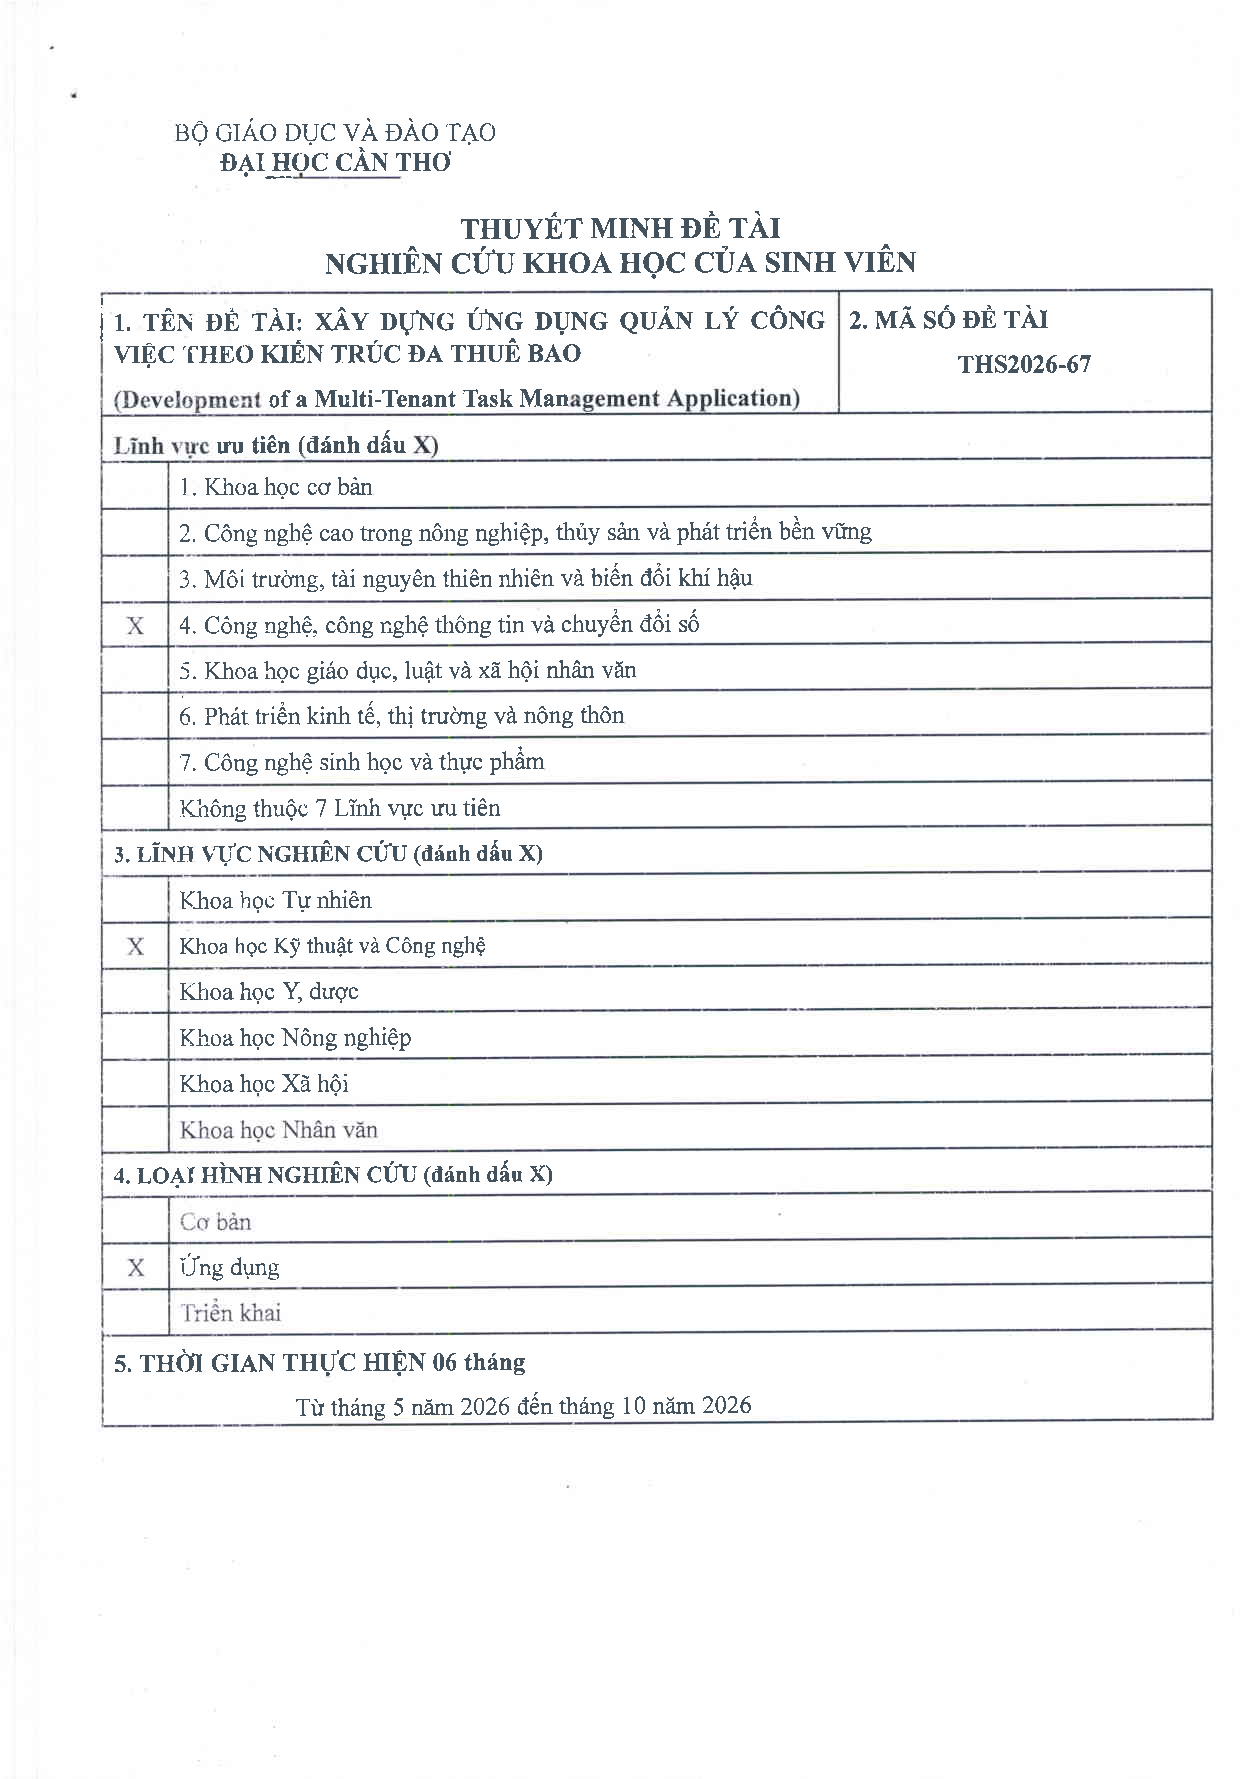
\includepdf[pages=-,pagecommand={}]{assets/approved-proposal.pdf}
% HinhThucBC 3.16: registered group I-III products, using real evidence PDFs.
% \includepdf[pages=-,pagecommand={}]{assets/product-evidence.pdf}
\clearpage\bookmarksetup{startatroot}\pdfbookmark[0]{Bản tin và báo cáo tóm tắt}{product-bulletins}
\pdfbookmark[1]{Bản tin tiếng Việt}{product-bulletin-vi}
\begin{officialform}[BulletinVI]
\FormHeading
\FormLine{Mã số đề tài: \ProjectCode}
\FormLine{Tên đề tài: \ProjectTitle}
\FormLine{Thời gian thực hiện: \ProjectPeriod}
\FormLine{Tổng kinh phí: \ProjectBudget}
\FormLine{Chủ nhiệm đề tài: \PrincipalName\ (\PrincipalPhone)}
\FormLine{Thành viên tham gia nghiên cứu: \ProjectMembers}
\FormLine{Cán bộ hướng dẫn: \SupervisorName\ (\SupervisorEmail)}
\FormLine{Tính cấp thiết: Nhu cầu sử dụng ứng dụng quản lý công việc và cộng tác trong môi trường đại học ngày càng tăng. Để phục vụ nhiều lớp học, nhóm nghiên cứu hoặc tổ chức trên cùng một nền tảng, ứng dụng cần nhận diện đúng từng thuê bao, bảo vệ dữ liệu riêng và duy trì hiệu năng khi dùng chung tài nguyên.}
\FormLine{Mục tiêu: Nghiên cứu, thiết kế và xây dựng ứng dụng quản lý công việc Kanban theo kiến trúc đa thuê bao; triển khai ứng dụng dưới dạng dịch vụ qua Internet và đánh giá tính an toàn, hiệu năng, khả năng tùy biến của kiến trúc.}
\FormLine{Phương pháp nghiên cứu: Tổng hợp và phân tích tài liệu; thiết kế kiến trúc từ yêu cầu nghiệp vụ; xây dựng nguyên mẫu; thực nghiệm có kiểm soát bằng các kịch bản kiểm thử cô lập dữ liệu, định danh, hiệu năng và tùy biến.}
\FormLine{Nội dung nghiên cứu: Nghiên cứu kiến trúc đa thuê bao; phân tích yêu cầu và thiết kế cơ chế định danh, cô lập dữ liệu, kiểm soát tải và tùy biến; xây dựng, triển khai ứng dụng Kanban; kiểm thử và đánh giá hệ thống.}
\FormLine{Kết quả đạt được: Xây dựng nguyên mẫu TenantFlow theo mô hình Pool cấp độ 3, triển khai trên AWS EC2. Trong thử nghiệm, 600 mẫu tiêm lỗi không ghi nhận rò rỉ dữ liệu chéo thuê bao; 1.500 yêu cầu luân phiên không phát hiện nhiễm bẩn ngữ cảnh. Với tải 80 người dùng ảo, p95 của các nhóm thuê bao thông thường đạt khoảng 242--277 ms; 19/19 lượt tạo thẻ có trường mở rộng được chấp nhận. p99 vẫn ở mức khoảng 1,99--2,45 giây và cần tiếp tục tối ưu.}
\FormLine{Ý nghĩa: Đề tài cung cấp mô hình tham khảo kết hợp kiến trúc đa thuê bao với một ứng dụng cộng tác cụ thể, đồng thời minh họa các đánh đổi giữa bảo mật dữ liệu, hiệu năng và chi phí dùng chung hạ tầng.}
\FormLine{Khả năng ứng dụng: Có thể dùng làm tài liệu tham khảo và nền tảng thử nghiệm cho ứng dụng quản lý công việc, dự án hoặc cộng tác trong trường đại học, doanh nghiệp vừa và nhỏ, nhóm khởi nghiệp.}
\end{officialform}

\clearpage\pdfbookmark[1]{Bản tin tiếng Anh}{product-bulletin-en}
\begin{officialform}[BulletinEN]\begin{english}
\FormHeading
\FormLine{Project code: \ProjectCode}
\FormLine{Project title: \ProjectTitleEnglish}
\FormLine{Duration: \ProjectPeriodEnglish}
\FormLine{Budget: \ProjectBudgetEnglish}
\FormLine{Coordinator: \PrincipalName\ (\PrincipalPhone)}
\FormLine{Members: \ProjectMembers}
\FormLine{Supervisor: \SupervisorName\ (\SupervisorEmail)}
\FormLine{Project rationale: Universities and organizations increasingly need task management and collaboration tools. A shared service must identify each tenant correctly, protect its data, and maintain service quality while tenants use common infrastructure.}
\FormLine{Objectives: To study, design, and develop a multi-tenant Kanban task management application; deploy it as an Internet-accessible service; and evaluate its data isolation, performance, and runtime customization.}
\FormLine{Methodology: Literature review and analysis; requirements-driven architecture design; prototype implementation; and controlled experiments covering identity and context integrity, data isolation, performance, and tenant-specific customization.}
\FormLine{Project activities: Review multi-tenant architectures; analyze requirements; design tenant identification, data isolation, rate limiting, caching, and customization mechanisms; build and deploy the Kanban application; conduct experiments and evaluate results.}
\FormLine{Research results: The project developed TenantFlow using a Level 3 Pool architecture and deployed it on AWS EC2. The Chapter 5 summary reports no cross-tenant data leaks in 600 fault-injection cases and no context contamination across 1,500 alternating tenant requests. With 80 workload virtual users (up to 82 including test users), p95 latency for regular tenants was approximately 242--277 ms. All 19 tested extended-field card creations succeeded. Tail latency at p99 remained approximately 1.99--2.45 seconds and requires further optimization.}
\FormLine{Research contribution: The study connects a multi-tenant architecture framework with a concrete Kanban application and evaluates identity controls, database row-level security, rate limiting, two-level caching, and runtime customization together in a deployed prototype.}
\FormLine{Potential applications: The prototype and findings can inform task management and collaboration services for universities, small and medium-sized businesses, and startup teams.}
\end{english}\end{officialform}

\clearpage\pdfbookmark[1]{Báo cáo tóm tắt tiếng Việt}{product-summary-vi}
\begin{officialform}[SummaryVI]
\FormHeading
\FormSection{1. Thông tin chung:}
\FormLine{Mã số đề tài: \ProjectCode}
\FormLine{Tên đề tài: \ProjectTitle}
\FormLine{Sinh viên chủ nhiệm đề tài: \PrincipalName}
\FormLine{Lớp: \PrincipalClass{} -- Khóa \PrincipalCohort; Trường/Khoa/Viện: \PrincipalUnit.}
\FormIndented{Năm thứ: \PrincipalYear\qquad Số năm đào tạo: \TrainingYears}
\FormLine{Người hướng dẫn: \SupervisorName}
\FormSection{2. Mục tiêu đề tài:}
\FormResultText{Nghiên cứu, thiết kế và xây dựng kiến trúc đa thuê bao cho ứng dụng quản lý công việc theo mô hình Kanban trong môi trường đại học. Đề tài tập trung vào định danh thuê bao, cô lập dữ liệu, kiểm soát tài nguyên dùng chung và bảo đảm tính nhất quán của trạng thái công việc; triển khai ứng dụng dưới dạng dịch vụ qua Internet và đánh giá tính khả thi, hiệu quả bằng thực nghiệm.}{Nghiên cứu và xây dựng kiến trúc đa thuê bao cho ứng dụng quản lý công việc trong môi trường đại học. Đề tài tập trung vào cơ chế định danh thuê bao, cô lập dữ liệu, kiểm soát tài nguyên dùng chung và bảo đảm tính nhất quán khi quản lý công việc. Nguyên mẫu được triển khai dưới dạng dịch vụ phần mềm có thể truy cập qua Internet và được đánh giá bằng thực nghiệm.}
\FormSection{3. Tính mới và sáng tạo:}
\FormResultText{Đề tài kết nối các cơ chế đa thuê bao ở nhiều tầng trong một ứng dụng Kanban cụ thể và kiểm chứng bằng thực nghiệm. Nguyên mẫu sử dụng mô hình Pool cấp độ 3, cho phép nhiều thuê bao dùng chung ứng dụng và cơ sở dữ liệu, đồng thời áp dụng các cơ chế bảo vệ định danh và dữ liệu. Ứng dụng hỗ trợ tùy biến theo từng thuê bao về nhận diện giao diện, quy tắc giới hạn công việc WIP và các trường dữ liệu mở rộng mà không cần thay đổi cấu trúc bảng dữ liệu.}{Đề tài kết nối các cơ chế đa thuê bao ở nhiều tầng trong một ứng dụng Kanban cụ thể, thay vì chỉ khảo sát từng kỹ thuật riêng lẻ. Nguyên mẫu áp dụng mô hình Pool cấp độ 3, trong đó nhiều thuê bao dùng chung ứng dụng và cơ sở dữ liệu nhưng được phân tách bằng ngữ cảnh định danh và chính sách bảo mật cấp dòng. Hệ thống cũng hỗ trợ tùy biến động theo từng thuê bao về giao diện, quy tắc WIP và trường dữ liệu mở rộng JSONB.}
\FormSection{4. Kết quả nghiên cứu:}
\FormResultText{Đề tài đã thiết kế, xây dựng và triển khai nguyên mẫu TenantFlow dưới dạng dịch vụ web. Hệ thống hỗ trợ nhiều tổ chức sử dụng chung hạ tầng, quản lý bảng Kanban và tùy biến quy trình theo từng thuê bao. Trong thử nghiệm, 1.500/1.500 yêu cầu luân phiên giữa các thuê bao giữ đúng ngữ cảnh; 600 mẫu tiêm lỗi không ghi nhận rò rỉ dữ liệu chéo. Với tải 80 người dùng ảo, độ trễ p95 của bốn nhóm thuê bao thông thường đạt khoảng 242--277 ms, dưới ngưỡng 500 ms. Hệ thống cũng kiểm chứng được khả năng giới hạn lưu lượng, áp dụng quy tắc WIP và lưu trường dữ liệu mở rộng. Độ trễ p99 còn khoảng 1,99--2,45 giây trong môi trường thử nghiệm một máy chủ và cần tiếp tục tối ưu.}{Đề tài đã xây dựng và triển khai nguyên mẫu TenantFlow với giao diện React, dịch vụ Spring Boot, PostgreSQL, Redis và Caddy trên AWS EC2. Kiểm thử ghi nhận 1.500/1.500 yêu cầu luân phiên giữa các thuê bao giữ đúng ngữ cảnh; 0 bản ghi rò rỉ trong 600 mẫu tiêm lỗi cơ sở dữ liệu. Với tải 80 người dùng ảo, p95 của bốn nhóm thuê bao thông thường đạt 242--277 ms, thấp hơn ngưỡng 500 ms đặt ra. Bộ giới hạn tốc độ từ chối 92,66\% yêu cầu vượt hạn mức của thuê bao gây nhiễu. Hệ thống cũng xử lý thành công các trường dữ liệu mở rộng và đồng bộ sự kiện làm mới bộ đệm qua Redis Pub/Sub. p99 còn khoảng 1,99--2,45 giây trong môi trường một máy chủ và cần tối ưu thêm.}
\FormSection{5. Sản phẩm:}
\FormLine{Ứng dụng web quản lý công việc Kanban theo kiến trúc đa thuê bao, triển khai dưới dạng dịch vụ qua Internet.}
\FormLine{Báo cáo tổng kết đề tài.}
\FormLine{Bản tin đề tài và báo cáo tóm tắt.}
\FormLine{Video clip giới thiệu đề tài, thời lượng tối đa 2 phút.}
\FormSection{6. Công bố khoa học từ kết quả nghiên cứu của đề tài, hoặc nhận xét, đánh giá của cơ sở đã áp dụng các kết quả nghiên cứu (nếu có):}
\begingroup
\setlength{\tabcolsep}{5.4bp}
\setlength{\arrayrulewidth}{.48bp}
\renewcommand{\arraystretch}{1}
\noindent\hspace*{\FormPublicationOffset}%
\begin{tabular}{|>{\centering\arraybackslash}p{\FormPublicationFirst}|P{135.03bp}|P{68.30bp}|P{63.24bp}|P{\FormPublicationIssue}|P{59.28bp}|}
\hline
\multicolumn{1}{|c|}{\textbf{Stt}} & \textbf{Tên bài báo} & \textbf{Tác giả/ nhóm tác giả} &
\textbf{Tên tạp chí} & \textbf{Số tạp chí} & \textbf{Năm xuất bản} \\
\hline
\multicolumn{6}{|l|}{Không} \\
\hline
\end{tabular}\par
\endgroup
\FormSection{7. Đóng góp về mặt kinh tế -- xã hội, giáo dục và đào tạo, an ninh, quốc phòng và khả năng áp dụng của đề tài:}
\FormResultText{Đề tài cung cấp mô hình tham khảo để thiết kế ứng dụng SaaS đa thuê bao, góp phần hỗ trợ chuyển đổi số trong quản lý công việc và cộng tác. Ứng dụng có thể hỗ trợ giảng viên, sinh viên và nhóm nghiên cứu theo dõi nhiệm vụ, dự án và tiến độ làm việc. Kết quả nghiên cứu cũng có thể sử dụng trong giảng dạy, học tập và làm cơ sở phát triển các ứng dụng đa thuê bao cho những lĩnh vực khác.}{Đề tài cung cấp mô hình tham khảo về cách tổ chức ứng dụng SaaS đa thuê bao và kiểm chứng các cơ chế định danh, cô lập dữ liệu, kiểm soát tải và tùy biến. Ứng dụng có thể hỗ trợ giảng viên, sinh viên và nhóm nghiên cứu quản lý nhiệm vụ, dự án và cộng tác. Kết quả cũng có thể làm tài liệu học tập, giảng dạy và nền tảng để phát triển các ứng dụng đa thuê bao trong lĩnh vực khác.}
\FormSection{8. Hiệu quả, phương thức chuyển giao kết quả nghiên cứu và khả năng áp dụng:}
\FormResultText{Kết quả nghiên cứu, tài liệu thiết kế và ứng dụng được tổng hợp để bàn giao cho Trường Công nghệ Thông tin và Truyền thông, Đại học Cần Thơ. Sản phẩm có thể dùng làm tài liệu tham khảo, phục vụ giảng dạy và nghiên cứu tiếp theo về kiến trúc phần mềm, dịch vụ SaaS và hệ thống đa thuê bao.}{Toàn bộ kết quả nghiên cứu được tổng hợp và bàn giao cho Trường Công nghệ Thông tin và Truyền thông, Đại học Cần Thơ. Ứng dụng và tài liệu có thể dùng làm tham khảo, giảng dạy và phát triển nghiên cứu tiếp theo về kiến trúc phần mềm, SaaS và hệ thống đa thuê bao.}

\end{officialform}

\clearpage\pdfbookmark[1]{Báo cáo tóm tắt tiếng Anh}{product-summary-en}
\begin{officialform}[SummaryEN]\begin{english}
\FormHeading
\FormSection{1. General information:}
\FormIndented{Project code: \ProjectCode}
\FormIndented{Project title: \ProjectTitleEnglish}
\FormIndented{Coordinator: \PrincipalName}
\FormIndented{Implementing institution: \PrincipalUnitEnglish}
\FormIndented{Duration: \ProjectPeriodEnglish.}
\FormSection{2. Objective(s):}
% V4 leaves this field empty; no new translation/summary is generated.
\PendingField{Objectives}
\FormSection{3. Creativeness and innovativeness:}
% Explain the original contribution.
\PendingField{Original contribution}
\FormSection{4. Research results:}
% Summarize supported findings.
\PendingField{Results}
\FormSection{5. Products:}
% List completed research products.
\PendingField{Products}
\FormSection{6. Effects, technology transfer means and applicability:}
% Describe demonstrated effects and transfer arrangements.
\PendingField{Effects and transfer}

\end{english}\end{officialform}

\end{document}
